% The U.S. Vote/OVF E2E-VIV Report

% Turning off "draft" mode on the report class turns off to do notes,
% chapter assignments, and completion percentages
\documentclass[oneside]{book}

\usepackage{pdfpages}

%\usepackage{times}
% Fourier for math | Utopia (scaled) for rm | Helvetica for ss | Latin Modern for tt
\usepackage{fourier} % math & rm
\usepackage[scaled=0.870]{helvet} % ss
\renewcommand{\ttdefault}{lmtt} %tt

\usepackage[hang]{footmisc}
\setlength{\footnotemargin}{2mm}

\usepackage{etoolbox}
\usepackage{ifpdf}
\usepackage{ifdraft}
\usepackage[utf8]{inputenc}
\usepackage[T1]{fontenc}
\usepackage{fnpct}
\usepackage{xcolor}
\usepackage{graphicx} % always include images, even in draft mode
\usepackage{wrapfig}
\usepackage{xspace}
\usepackage{colortbl}
\usepackage{longtable}
\usepackage{tabu}
\usepackage[inline]{enumitem}
\usepackage[final]{listings} % always include listings, even in draft mode

% Bibliography equipment for fancier citations of websites etc
\usepackage[%
  backend=bibtex      % biber or bibtex
%,style=authoryear    % Alphabeticalsch
 ,style=numeric-comp  % numerical-compressed
%,sorting=none        % no sorting
 ,sortcites=true      % some other example options ...
 ,block=none
 ,indexing=false
 ,citereset=none
 ,isbn=true
 ,url=true
 ,doi=true            % prints doi
 ,natbib=true         % if you need natbib functions
]{biblatex}
\DefineBibliographyStrings{english}{%
  bibliography = {References},
}
\addbibresource{bibliography.bib}

\setcounter{biburllcpenalty}{7000}
\setcounter{biburlucpenalty}{8000}

% BON listing style
\usepackage{color}
\usepackage{listings}


\newcommand{\comment}[1]{\textcolor{red}{#1}}
\definecolor{keywordcolor}{rgb}{0.5,0,0.33}
\definecolor{identifiercolor}{rgb}{0,0,0.75}
\definecolor{commentcolor}{rgb}{0.25,0.5,0.37}
\definecolor{commentcolor}{rgb}{0.3,0.3,0.3} 

\lstdefinelanguage{bon} {
  morekeywords={class_chart,indexing,explanation,part,query,command,constraint,
  end,deferred,effective,persistent,require,ensure,invariant,feature,class,
  static_diagram,component,old,not,inherit,delta,for_all,such_that,it_holds,Current,
  Lockset,when,monitors_for,max,concurrency,concurrent,guarded,locks,special,
  failure,sequential,atomic},
  morekeywords={[2]BOOLEAN,INTEGER,REAL,SEQUENCE}, 
  morekeywords={[3]},
  morecomment=[l]{--}, morestring=[b]", morestring=[d]'
  }[keywords,comments,strings]

\lstdefinestyle{bon}{language={bon},showstringspaces={false},
  basicstyle={\small\ttfamily\mdseries},
  keywordstyle={\color{keywordcolor}},
  keywordstyle={[2]\color{black}\bfseries},
  keywordstyle={[3]\color{black}\bfseries},
  identifierstyle={\color{identifiercolor}},
  commentstyle={\color{commentcolor}},
  frame=none}

\lstdefinestyle{bonbw}{language={bon},showstringspaces={false},
  basicstyle={\small\ttfamily\mdseries},
  keywordstyle={\color{black}},
  keywordstyle={[2]\color{black}\bfseries},
  keywordstyle={[3]\color{black}\bfseries},
  identifierstyle={\color{black}\mdseries},
  commentstyle={\color{black}},
  frame=none,
  columns=fullflexible,
  breaklines=true}
\lstset{style=bon, columns=fullflexible, keepspaces=true, frame=lines,
  captionpos=b, numbers=none} 

% custom colors
\colorlet{darkgreen}{green!35!black}
\colorlet{darkred}{red!45!black}

% shades of red and green that are distinguishable even with the most common
% kinds of color blindness
\colorlet{accessiblegreen}{green!55!black!70!blue!40!white}
\colorlet{accessiblered}{red!80!black!80!yellow!30!white}

% E2E-VIV Report Colors
\definecolor{DarkGreen}{HTML}{00AB8E}
\definecolor{DARKGREEN}{HTML}{00AB8E}
\definecolor{LightGreen}{HTML}{A4D65E}%{B3D78B}
\definecolor{DarkBlue}{HTML}{041E42}%{002D62}
\definecolor{Red}{HTML}{9D2235} %{B20738}

\usepackage[margin=1in]{geometry}
\usepackage[defaultlines=4,all]{nowidow}
\usepackage[parfill]{parskip}

%% To Do Notes
\usepackage[obeyDraft, colorinlistoftodos, textwidth=\marginparwidth]{todonotes}

% individual colors for To Dos, feel free to change yours
\colorlet{tododmz}{green!50}
\colorlet{todokiniry}{red!50}
\colorlet{tododmwit}{orange!50}
\colorlet{todojkr}{blue!50}
\colorlet{todojrk}{orange!50!yellow}
\colorlet{todoprobinson}{purple!50}
\colorlet{todoacf}{cyan!50}
\colorlet{todogeneric}{yellow!50}

\newcounter{todocounter}
\newcommand{\todocount}[2][]{\stepcounter{todocounter}\todo[#1]{\thetodocounter:
    #2}}

% individual commands for To Dos
% usage: \todo<username>{Something to do.}
\newcommand{\tododmz}[1]{\todocount[color=tododmz]{#1}}
\newcommand{\todokiniry}[1]{\todocount[color=todokiniry]{#1}}
\newcommand{\tododmwit}[1]{\todocount[color=tododmwit]{#1}}
\newcommand{\todojkr}[1]{\todocount[color=todojkr]{#1}}
\newcommand{\todojrk}[1]{\todocount[color=todojrk]{#1}}
\newcommand{\todoprobinson}[1]{\todocount[color=todoprobinson]{#1}}
\newcommand{\todoacf}[1]{\todocount[color=todoacf]{#1}}
\newcommand{\todogeneric}[1]{\todocount[color=todogeneric]{#1}}

\ifpdf
\usepackage[draft=false,pdftex,colorlinks=true,urlcolor=DarkGreen,linkcolor=DarkGreen,citecolor=DarkGreen,bookmarks=false]{hyperref}
\else
\usepackage[dvips]{hyperref}
\fi


% define a macro \Autoref to allow multiple references to be passed to
% \autoref
\makeatletter
\newcommand\Autoref[1]{\@first@ref#1,@}
\def\@throw@dot#1.#2@{#1}% discard everything after the dot
\def\@set@refname#1{%    % set \@refname to autoefname+s using \getrefbykeydefault
    \edef\@tmp{\getrefbykeydefault{#1}{anchor}{}}%
    \def\@refname{\@nameuse{\expandafter\@throw@dot\@tmp.@autorefname}s}%
}
\def\@first@ref#1,#2{%
  \ifx#2@\autoref{#1}\let\@nextref\@gobble% only one ref, revert to normal \autoref
  \else%
    \@set@refname{#1}%  set \@refname to autoref name
    \@refname~\ref{#1}% add autoefname and first reference
    \let\@nextref\@next@ref% push processing to \@next@ref
  \fi%
  \@nextref#2%
}
\def\@next@ref#1,#2{%
   \ifx#2@ and~\ref{#1}\let\@nextref\@gobble% at end: print and+\ref and stop
   \else, \ref{#1}% print  ,+\ref and continue
   \fi%
   \@nextref#2%
}

% the short version of the report has a table of contents with one line on
% the next page; this scrunches the top of the table to avoid that bad break
\iftechreport\else
\let\@starttocold\@starttoc
\renewcommand{\@starttoc}[1]{
  \ifstrequal{#1}{toc}{\vspace*{-6ex}}{}
  \@starttocold{#1}
}
\fi
\makeatother

\usepackage{lipsum}
\usepackage{soul}

\newcommand\recommendation[2]{%
  \vspace{12pt}%
  \colorbox{DarkGreen}{%
    \textbf{\emph{\textcolor{white}{Recommendation: \uppercase{#1}}}}%
  }%
  \ \textbf{#2}%
}
\newcommand\withicon[2]{%
  \begin{wrapfigure}[1]{r}{0.625in}%
    \vspace*{1.5ex}%
    \includegraphics[width=0.75in]{#1}%
  \end{wrapfigure}%
  \paragraph{}%
  \vspace*{-\parskip}%
  #2
  \vspace*{3ex}%
}

% Modify the autoref names to be capitalized and not sub-sub-subby.
\renewcommand*{\chapterautorefname}{Chapter}
\renewcommand*{\sectionautorefname}{Section}
\renewcommand*{\subsectionautorefname}{Section}
\renewcommand*{\subsubsectionautorefname}{Section}

% Various definitions, from Aggelos E2E spec

\newcommand{\func}[1][\relax]{\ensuremath{\mathcal{F}_{\mathsf{#1}}}}
\newcommand{\fl}[1]{\mbox{\( \lfloor #1 \rfloor \)}}
\newcommand{\pair}[2]{\mbox{\(\langle #1,#2 \rangle\)}}

\newcommand{\mc}{\mathcal}
\newcommand{\Pro}{\mbox{\( \mathbf{ Prob } \)}}

\def\squareforqed{\hbox{\(\blacksquare\)}}
\def\qed{\ifmmode\squareforqed\else{\unskip\nobreak\hfill\penalty50\hskip1em\null\nobreak\hfil\squareforqed\parfillskip=0pt\finalhyphendemerits=0\endgraf}\fi}

\newtheorem{theorem}{Theorem}[section]
\newtheorem{assumption}{Complexity Assumption}
\newtheorem{lemma}[theorem]{Lemma}
\newtheorem{remark}{Remark}
\newtheorem{claim}{Claim}
\newtheorem{fact}[theorem]{Fact}
\newtheorem{definition}[theorem]{Definition}
\newtheorem{corollary}[theorem]{Corollary}
\newtheorem{proposition}[theorem]{Proposition}
\newenvironment{proof}{\noindent {\em Proof.}}{\medskip}

\def\PPT{{\rm PPT} }
\def\ff{\mathbb{F}}
\def\sbs{\subseteq}
\def\zz{\mathbb{Z}}
\def\E{\mathsf{E}}

%Functionalities
\newcommand{\fete}{\func[e2e]}%
\newcommand{\fbb}{\func[bb]}%
\newcommand{\fsauth}{\func[sauth]}%
\newcommand{\fauth}{\func[auth]}%
\newcommand{\fmail}{\func[mail]}%
\newcommand{\frnd}{\func[rnd]}%

%Parties
\def\EA{\mathsf{EA}}
\def\VT{\mathsf{V}}
\def\RB{\mathsf{RB}}
\def\VC{\mathsf{VC}}
\def\AU{\mathsf{AU}}

\def\Exec{\mathsf{Exec}}


%Commands
\def\Create{\mathtt{Create}}
\def\Sample{\mathtt{Sample}}
\def\FakeBallot{\mathtt{FakeBallot}}
\def\Deliver{\mathtt{Deliver}}
\def\Corrupt{\mathtt{Corrupt}}
\def\Verify{\mathtt{Verify}}
\def\Tally{\mathtt{Tally}}
\def\Vote{\mathtt{Vote}}
\def\RecordVote{\mathtt{RecordVote}}
\def\Append{\mathtt{Append}}
\def\Read{\mathtt{Read}}
\def\Send{\mathtt{Send}}
\def\Mail{\mathtt{Mail}}
\def\Audit{\mathtt{Audit}}
\def\VBB{\mathtt{VBB}}
\def\SendInit{\mathtt{SendInit}}
\def\GetRnd{\mathtt{GetRnd}}
\def\Select{\mathtt{Select}}
\def\RecordTally{\mathtt{RecordTally}}
\def\ReadTally{\mathtt{ReadTally}}
\def\Receipt{\mathtt{Receipt}}
\def\Result{\mathtt{Result}}
\def\ElectionFail{\mathtt{ElectionFail}}

% Modified Chapter/Section/Subsection Headings And Text Formats
\usepackage[compact,explicit]{titlesec}

\renewcommand{\chaptername}{CHAPTER}
\titleformat{\chapter}[display]{\Huge\bfseries\sffamily}{\textcolor{DarkGreen}{\chaptertitlename\ \thechapter}}{20pt}{\textcolor{DarkGreen}{\MakeUppercase{#1}}}
\titleformat{\section}[display]{\Large\bfseries\sffamily}{}{0em}{\textcolor{DarkGreen}{\thesection\quad\MakeUppercase{#1}}}
\titleformat{name=\subsection,numberless}[display]{\large\bfseries\sffamily}{}{0em}{\textcolor{DarkGreen}{\MakeUppercase{#1}}}
\titleformat{\subsection}[display]{\large\bfseries\sffamily}{}{0em}{\textcolor{DarkGreen}{\thesubsection\quad\MakeUppercase{#1}}}
\titleformat{name=\subsection,numberless}[display]{\bfseries\sffamily}{}{0em}{\textcolor{DarkGreen}{\MakeUppercase{#1}}}
\titleformat{\subsubsection}[display]{\bfseries\sffamily}{}{0em}{\textcolor{DarkGreen}{\MakeUppercase{#1}}}
\titleformat{\paragraph}[runin]{\bfseries\sffamily}{}{0em}{\textcolor{DarkGreen}{\MakeUppercase{#1}}}

\usepackage{tocloft}
\usepackage{fancyhdr}

% light-grey headers with section names/subsections, footers with page numbers
\fancyhead{}
\fancyhead[L]{\sffamily\small\textcolor{gray}{\leftmark}}
\fancyhead[R]{\sffamily\small\textcolor{gray}{\rightmark}}
\fancyfoot{}
\fancyfoot[C]{\sffamily\thepage}

\fancypagestyle{plain}{
  \fancyhf{}
  \renewcommand{\headrulewidth}{0pt}
  \fancyfoot[C]{\sffamily\thepage}
}

% redefine boldface to sans-serif and green
\DeclareTextFontCommand{\textbf}{\bfseries\sffamily\color{DarkGreen}}
% redefine italics to sans-serif and green (two forms)
\DeclareTextFontCommand{\textit}{\itshape\sffamily\color{DarkGreen}}
\DeclareTextFontCommand{\emph}{\itshape\sffamily\color{DarkGreen}}

% end of preamble

\begin{document}
% The title page has no visible page number, and the report resets page
% numbering on the next page so that the visible page numbers start from 1.
% One unfortunate side effect of this is that hyperref sees two different
% pages both named "1" and gets confused. See also
% http://tex.stackexchange.com/q/18924/16779
\frontmatter

\hypersetup{pageanchor=false}
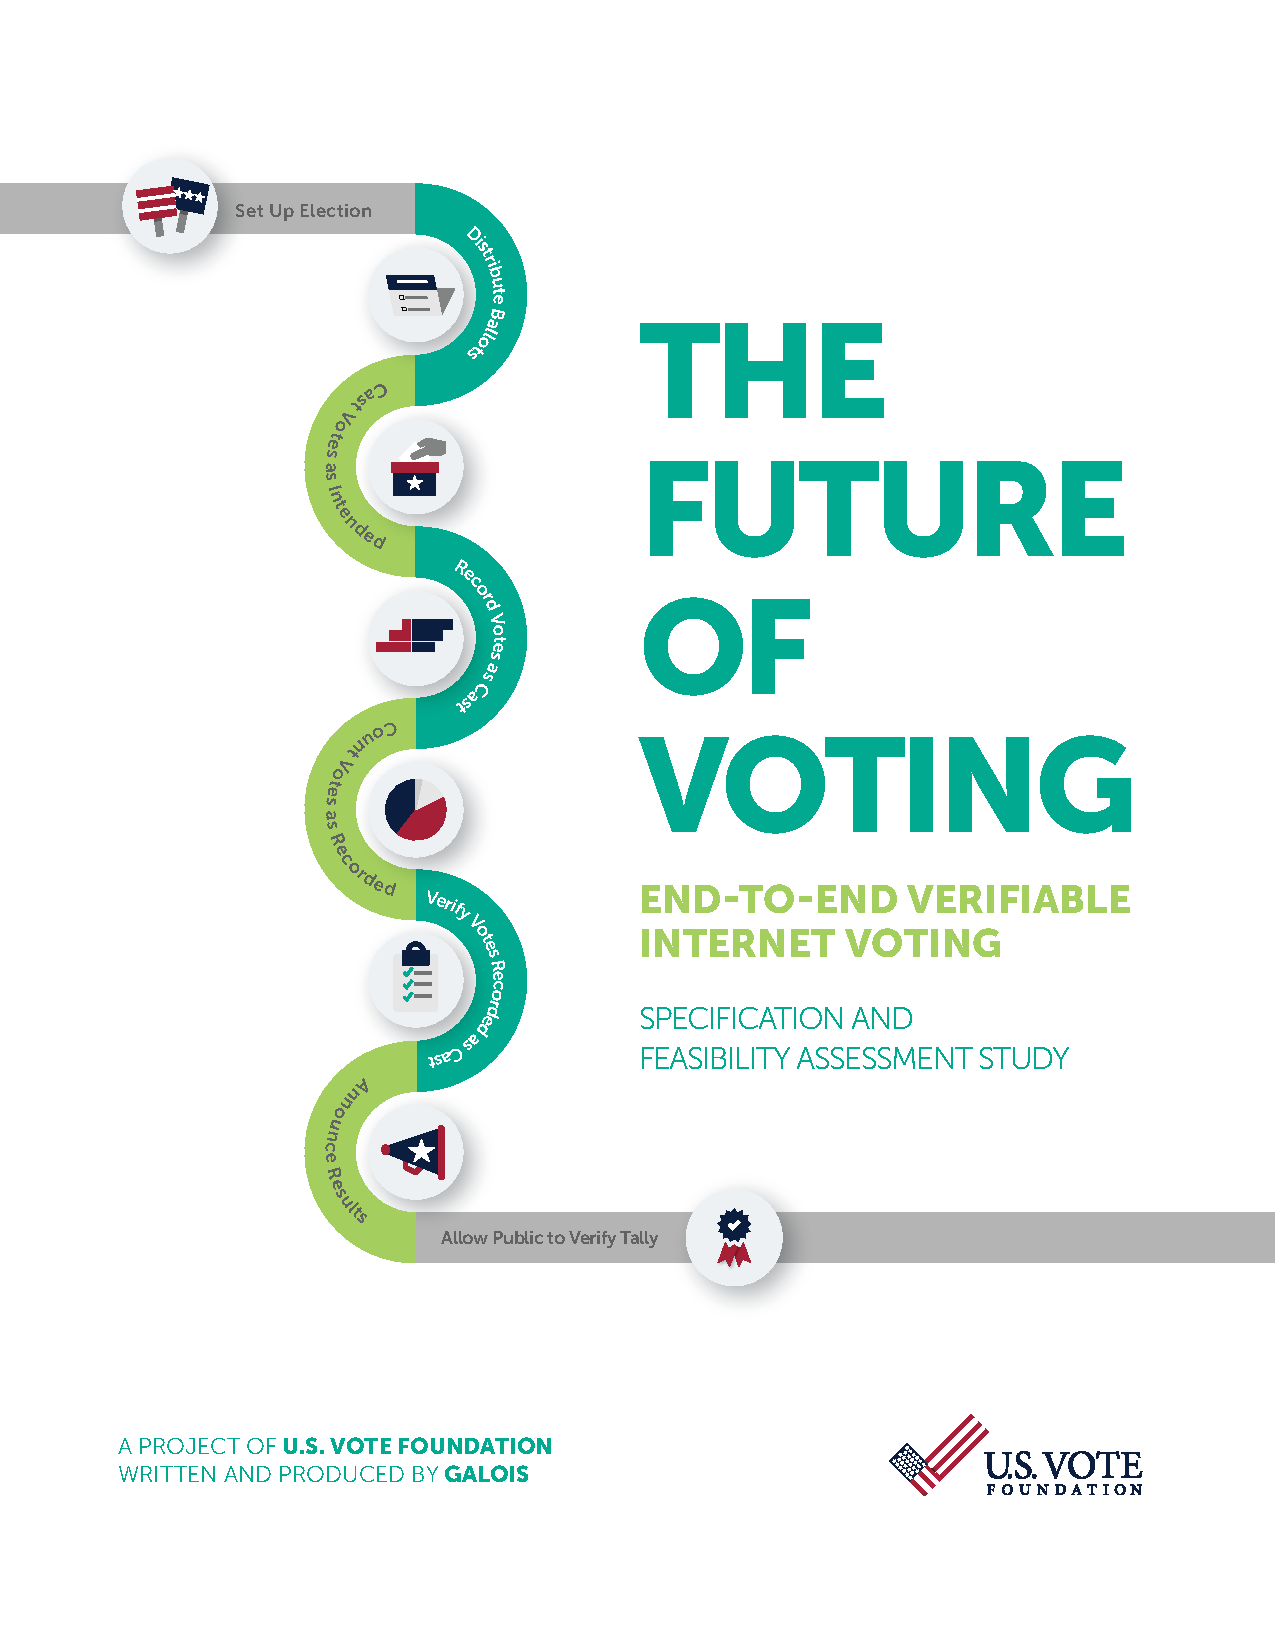
\includepdf[pages=1-5]{executive_summary}
% \hypersetup{pageanchor=false}
% \maketitle
% \hypersetup{pageanchor=true}

\renewcommand{\contentsname}{\textcolor{DarkGreen}{CONTENTS}}
\renewcommand{\cfttoctitlefont}{\Huge\bfseries\sffamily}
\renewcommand{\cftchapfont}{\bfseries\sffamily}
\renewcommand{\cftsecfont}{\sffamily}
\renewcommand{\cftsubsecfont}{\sffamily}
\renewcommand{\cftsubsubsecfont}{\sffamily}
\renewcommand{\cftfigfont}{\sffamily}
\renewcommand{\cfttabfont}{\sffamily}
\renewcommand{\cftchappagefont}{\bfseries\sffamily}
\renewcommand{\cftsecpagefont}{ \sffamily}
\renewcommand{\cftsubsecpagefont}{ \sffamily}  
\renewcommand{\cftsubsubsecpagefont}{ \sffamily}
\renewcommand{\cftfigpagefont}{ \sffamily}
\renewcommand{\cfttabpagefont}{ \sffamily}
 
\pagestyle{fancy}
\fancyhead[R]{}
\tableofcontents

\iftechreport\else
\vfill

This document is an abridged version, prepared for non-technical audiences.
The full report, ``THE FUTURE OF VOTING: End-To-End Verifiable Internet
Voting'', is available from \url{https://www.usvotefoundation.org/E2E-VIV},
and contains additional details on cryptographic foundations, architecture,
and rigorous software engineering practices.
\fi

\clearpage
\fancyhead[R]{\sffamily\small\textcolor{gray}{\rightmark}}
\ifdraft{\addcontentsline{toc}{chapter}{\ \ \ \ \hl{Note: Names following
    chapter titles are the currently-assigned writers; percentages
    following writer names are very rough estimates of the
    approximate percentage of completion. Some material factored 
    into the percentages may not yet appear in the generated report 
    because it needs to be brought in from external sources.} \\ \ \\
  List of To Do Items}
% temporarily here, so we have a centralized list of all the todo
% items in the document
\listoftodos[List of To Do Items]
}{}
%\chapter{Executive Summary\ifdraft{ (Joe K./Susan) (0\%)}{}}
\label{chapter:executive_summary}

\begin{itemize}
\item framing of project \& methodology
\item who is involved
\item who funded it
\item goals and deliverables
\item feasibility
\item recommendation
\item ``why now'' coupled to history
\item why do existing systems suck
\item ``how'' what is E2E VIV (illustration)
\item five key mandatory properties: end-to-secure, verifiability,
  100\% accessible, high-assurance, transparent
\item crypto framing
\item architectural framing
\item RSE framing
\item conclusion and future phases
\end{itemize}
 % Joe K./Susan
\mainmatter
\hypersetup{pageanchor=true}
\chapter*{Acknowledgments}
\addcontentsline{toc}{chapter}{Acknowledgments}
\label{chapter:acknowledgments}

This project and report would not have been possible without the
commitment and tireless hard work of the team at Galois, Inc. Our
special acknowledgment and appreciation goes most especially to Joseph
Kiniry, who brought his decades of knowledge, skill, experience, and
leadership to the project, broadened its scope and led the technical
team and writing; and with him, the Galois team members Daniel
Zimmerman, Daniel Wagner, Philip Robinson, Adam Foltzer, Shpatar
Morina, and Leah Daniels. We are indebted to CEO Rob Wiltbank for the
Galois engineering contribution and the long leash he gave to this
project.

We would also like to thank the research and technical members of the
E2E-VIV Project Team for their contributions to this project from its
conception to its completion, with special thanks to Josh Benaloh,
Candice Hoke, Keith Instone, David Jefferson, Doug Jones, Aggelos
Kiayias, Judy Murray, Ron Rivest, Barbara Simons, and Poorvi Vora.

Equally vital and integral to this report were the reflections,
insights and advice from election officials who joined our team, most
especially Lori Augino, Judd Choate, Dana Debeauvoir, Mark Earley,
Stuart Holmes, Dean Logan, Tammy Patrick, Roman Montoya, and Lois
Neuman.  We also thank Sean Beggs, Randall Trzeciak, and Andrew
Wasser, Carnegie Mellon University, Heinz College Master of
Information Systems Management for their support through the CMU ISM
Capstone Program.

We are grateful for the generous financial support of the Democracy
Fund, as well as their support of collaborative efforts in the realm
of civic tech development.


\begin{tabbing}
\` \sffamily\bfseries\textcolor{DarkGreen}{Susan Dzieduszycka-Suinat} \\
\` \sffamily\textcolor{DarkGreen}{President and Chief Executive Officer} \\
\` \sffamily\textcolor{DarkGreen}{U.S. Vote Foundation}
\end{tabbing}

\vspace{\fill}

For additional information on U.S. Vote Foundation, please visit
\url{www.usvotefoundation.org}.   

For additional information on the Overseas Vote Initiative, please
visit \url{www.overseasvote.org}. 

For additional information on Galois, Inc., please visit
\url{www.galois.com}.

For additional information on the Democracy Fund, please visit
\url{www.democracyfund.org}.

%%% Local Variables:
%%% mode: latex
%%% TeX-master: "report"
%%% End:
 
\chapter{Introduction\ifdraft{ (Joe K./Susan) (70\%)}{}}
\label{chapter:introduction}

%=====================================================================
\section{The E2E VIV Project}

%~~~~~~~~~~~~~~~~~~~~~~~~~~~~~~~~~~~~~~~~~~~~~~~~~~~~~~~~~~~~~~~~~~~~~
\subsection{Situation}

In March 2013, Overseas Vote Foundation’s President and CEO began a
discussion with a small group of experienced, election integrity
technology advocates about how, if faced with having to specify an
Internet voting system, they would respond. Security concerns being
the primary reason for their general opposition to what they deemed
inadequate efforts of others to do so to date, it was nonetheless
agreed that taking on the question was crucial at the time. 

Gridlock is not unique to Washington politics, it is quite well known
around the topic of Internet Voting in the U.S. The scientific
community, federal agencies, cyber security specialists and certain
organized activists have strongly advised against exposing the ballots
of the most powerful nation on earth to the seemingly endless range of
cyber threats, which run rampant on today’s Internet. 

Nevertheless, faced with ongoing challenges to serve their
constituencies in modern and efficient ways, and having experienced
the everyday efficiencies of technology throughout their lives, when
seeking new and improved election systems, election officials often
want to consider Internet-based technologies. In the current climate
of economic austerity, innovation in elections is rare. Our election
officials are trapped in a technology no-man’s land of ongoing support
payments for outdated voting systems, compounded by no means of
certifying new voting systems they would like.

Election integrity advocates cite that secure, tested, certified
remote voting systems that election officials envision aren’t
available. The scientific community does not consider online ballot
return systems secure, nor are they certified. As a result, email has
become the default stopgap method for moving ballots online, although
it does not provide any of the benefits that a secure, full-featured
voting system would provide. Email is demonstrably weak on security,
yet election officials and voters are using it regularly to transmit
ballots because viable alternatives are not available. Examination of
new and better ways to use technology to meet specific voting needs,
for example, that of the remote overseas citizen, military and
disabled is needed. 

Existing vendors of Internet voting technologies, whose systems are
neither tested nor certified, would like to openly market and sell
their systems within the U.S. and not face the resistance of the
election integrity advocates. No agreement on how to proceed, a
years-long history of mediocre attempts, ongoing animosity between
stakeholder parties, and a general lack of research on the current
questions could well-describe the situation.

%~~~~~~~~~~~~~~~~~~~~~~~~~~~~~~~~~~~~~~~~~~~~~~~~~~~~~~~~~~~~~~~~~~~~~
\subsection{A Proposed Solution}

Within this climate, a project proposal was written and funding
provided by The Democracy Fund, a Washington D.C. based philanthropic
organization whose stated objective is to “...invest in organizations
working to ensure that our political system is responsive to the
priorities of the American public and has the capacity to meet the
greatest challenges facing our country.” 

A project intent on examining the future of voting and how it might be
executed securely online fit neatly into the strategic purview of the
fund; one that approached the question of Internet-voting from a
research perspective, that sought to fill in the gaps of the many open
questions plaguing the discussion was regarded by the supporting
organization as a positive endeavor. 

According to Joe Goldman, Director of the Democracy Fund, “The
significance of this project will be in its ability to break open the
conversation from its current stalemate and include all sides in a
constructive project to openly examine and research what is really
needed by voters and election officials, and to determine whether this
form of voting can meet those needs and still guarantee security of
the election. Equally important, it will identify potential tradeoffs
and shortcomings that represent the diverse range of values we hold
dear in our elections.”

On December 19, 2013, Overseas Vote Foundation\footnote{Since the
  start of the study, Overseas Vote Foundation has been renamed as
  “Overseas Vote”, an initiative of U.S. Vote Foundation.} (OVF), a
nonpartisan, nonprofit organization dedicated to overseas and military
voter participation announced the launch of the project, which was
called the End-to-End Verifiable Internet Voting: Specification and
Feasibility Assessment Study (E2E VIV Project). Its stated aim was to
examine a form of remote voting that enables a so-called “end-to-end
verifiability” (E2E) property. A unique team of experts in computer
science, usability, and auditing together with a selection of local
election officials from key counties around the U.S. assembled for the
study.

They agreed to focus their efforts to produce a system specification
and set of testing scenarios, which if they meet the requirements for
security, auditability, and usability, would then be placed in the
public domain. At the same time, their intent was to demonstrate that
confidence in a voting system is built on a willingness to verify its
security through testing and transparency. 

There is an historical misunderstanding in the U.S. election community
that the E2E VIV Project aimed to correct: that our country’s best
scientists are not against technology advancements, nor are they
inherently at odds with the election officials who seek technology
improvements to meet their administrative challenges. Rather, that the
U.S. scientific community takes issue with unproven claims of security
regarding existing systems that are not publicly tested or vetted. The
study aimed to recalibrate this situation. 

The group of scientific leaders on the project has often pointed out
security vulnerabilities in past systems, however, in the face of the
E2E VIV Project, they agreed on one thing: that if Internet Voting
(IV) does happen, it should be in a system that takes advantage of
end-to-end verifiability and auditability.

%~~~~~~~~~~~~~~~~~~~~~~~~~~~~~~~~~~~~~~~~~~~~~~~~~~~~~~~~~~~~~~~~~~~~~
\subsection{Definition}

The term E2E is often used casually without
precision. E2E-verifiability is considered a property of an election
and for the purposes of the study, an E2E-verifiable election has two
important components: first, that voters can individually check that
their ballots are cast as they intend; and second, that anyone can
check that all of the cast ballots have been accurately
tallied\footnote{Definition from Dr.~Josh Benaloh, Senior
  Cryptographer at Microsoft Research.}.

While systems of this nature have been developed in the past, none
have been broadly used or successfully commercialized; the E2E VIV
Project would make a concerted effort to be informed by these past
efforts and build upon them as appropriate. Usability factors were
also considered from the outset of the study to address the
significant challenges faced by remote and disabled voters when using
such systems to participate. A viable outcome of this study with
respect to security, auditability, and usability is intended to enable
development efforts to ensue.

For those concerned with election integrity, there is a justifiably
negative reflex in response to IV: it takes all of the problems with
current remote voting systems and adds all of the problems and
security vulnerabilities of the Internet.  

The E2E VIV Project sought to potentially make the case that use of
the Internet enables and facilitates the introduction of
E2E-verifiability (E2EV) and that the benefits of E2EV may be able to
overcome the vulnerabilities introduced by using the Internet. No
participant on this project discounted the concerns of voting over the
Internet, nor did or do they view E2EV as a magic sauce that makes the
Internet secure. Nevertheless they believe that E2EV warrants
examination in regards to the properties it achieves. These properties
are achieved even when votes are cast on untrusted devices like PCs
and transmitted over an untrusted medium such as the Internet.

The E2E VIV Project does not attempt to make the Internet
secure. Instead, E2EV negates many (although not all) of the risks of
voting via the Internet while introducing substantial new benefits
that are not found in currently deployed voting systems.

%=====================================================================
\section{Goals and Objectives}

%~~~~~~~~~~~~~~~~~~~~~~~~~~~~~~~~~~~~~~~~~~~~~~~~~~~~~~~~~~~~~~~~~~~~~
\subsection{Shared Goals}

Election officials and scientists involved in elections \textbf{share}
the overall goals: that voting systems can be proven secure,
auditable, verifiable, and accessible.

This project is evidence that the needs and requests of election
officials to explore optimum ways of serving remote voters are of deep
concern to the scientific community, that they have a great motivation
to address these questions when given a constructive opportunity to do
so, and that they would like to work together, not at opposite ends,
to examine the possibilities in this realm.

%~~~~~~~~~~~~~~~~~~~~~~~~~~~~~~~~~~~~~~~~~~~~~~~~~~~~~~~~~~~~~~~~~~~~~ 
\subsection{Project Goal}

Our goal is to specify and define a system and its testing scenarios
for an online voting method that can provide both security and
confidence to voters that their selections are accurately recorded and
counted. Our assertion is that E2E-verifiability negates many,
although not all, of the risks of voting via the Internet while
introducing substantial new benefits that are not found in currently
deployed voting systems.

The project team presumes that if E2E VIV is a possible answer, or a
step toward one, we will find out and we will see if it can answer the
needs of many voters and election officials. If not, we will still
gain specific knowledge about the shortcomings, which can be further
acted upon in the future. 

%~~~~~~~~~~~~~~~~~~~~~~~~~~~~~~~~~~~~~~~~~~~~~~~~~~~~~~~~~~~~~~~~~~~~~
\subsection{Additional Objectives}

Presentation and discussion of the report with key stakeholders,
integrating their feedback, and garnering their cceptance of the
report (see below in Success section) are additional core objectives
of the project. 

%~~~~~~~~~~~~~~~~~~~~~~~~~~~~~~~~~~~~~~~~~~~~~~~~~~~~~~~~~~~~~~~~~~~~~
\subsection{Deliverables}

The main deliverable of the E2E VIV Project is the development of a
``whole product solution'' specification (or simply specification for
short) for a trustworthy E2E VIV election system.

We have produced a report presenting a system specification to create
a secure E2E VIV system, a set of testing specifications to
demonstrate the security, a set of guidelines for system usability,
accessibility, and testing. Additional topics and analyses may be
considered and discussed in the report, such as legal and
administrative challenges, and ballot secrecy, privacy, and
confidentiality.

%~~~~~~~~~~~~~~~~~~~~~~~~~~~~~~~~~~~~~~~~~~~~~~~~~~~~~~~~~~~~~~~~~~~~~
\subsection{A First Step}

This project represents step one in an examination of whether one day
this might be possible. Our current plan is to examine the potential
for an E2E VIV remote voting system together with election officials,
taking into close account their needs and the needs of disabled
voters. If a system can one day be developed based on these
principles, then we want to know. We need the answers that this
project will bring before we can say whether we, or anyone, will build
any new system. A viable outcome of this study with respect to
security, auditability, and usability will enable development efforts
to ensue.

%~~~~~~~~~~~~~~~~~~~~~~~~~~~~~~~~~~~~~~~~~~~~~~~~~~~~~~~~~~~~~~~~~~~~~
\subsection{Success}

Beyond judging the outcome – the fact that this project takes a
research and testing-based approach to a problem that has been “in
stalemate mode” will result, we believe, in stimulating election
development overall. The election industry is operating in a
traditional paradigm with only a few vendors able to survive, albeit
demand to move away from outdated, expensive, hardware-oriented
solutions.

It would be considered a success to specify a system and testing for a
usable, secure E2E verifiable remote voting technology, to identify
its strengths and weaknesses and reasons to pursue or not pursue this
approach to remote and/or disabled citizen voting.

However, from the beginning is was clear that if the project
determines that the technology is weak and should not be developed, it
would be a different outcome, but also one with many useful
implications. 

Success of the project can only be determined if the specification is
one that is: 1)~supported by the vast majority the expert teams,
including the technical, usability, testing, and research teams;
2)~endorsed by the vast majority of the advisory council, and;
3)~endorsed by the major stakeholders in elections administration as
represented by the project's local election officials.

Additionally, the E2E VIV Project expects to receive support and
endorsement from many members of the electronic voting activism
community, as represented by key members of the Election Verification
Network and the Verified Voting Foundation.

The specification will be of a form with sufficient detail such that
the following requirements are fulfilled:
\begin{description}
\item[Independent Implementation] The specification must be of
  sufficient detail and clarity that an implementation of the election
  system must be possible by an independent party without extensive
  dialog with participants in the project.
\item[Independent Validation] It must be possible for a moderately
  proficient IT expert to objectively determine, in a reasonable time
  frame with reasonable cost, if any election system constructed which
  claims to fulfill the specification.
\item[Evidence-Based Decisions] Every decision made in the crafting of
  the specification must be objectively justifiable and the evidence
  for the decision must be traceable. 
\end{description}

%~~~~~~~~~~~~~~~~~~~~~~~~~~~~~~~~~~~~~~~~~~~~~~~~~~~~~~~~~~~~~~~~~~~~~
\subsection{Scope}

The original project was tightly limited to involve system
specification and testing only. No system development was envisioned
in this phase beyond mockups to help test usability. However, this
changed early on in the project when Joe Kiniry of Galois, Inc. came
on board to manage the project and its team. 

The Galois engineers brought significant expertise to the project and
set about to develop a set of rigorous engineering artifacts
``demonstrators'' fit for refinement into a working election system, and
against which third parties can perform independent validation and
verification. According to Galois, demonstrators are technical
artifacts from the point of view of definition and constructions, but
non-technical artifacts from the point of view of
demonstration. Galois suggests that all demonstrators developed using
Galois IR\&D funding be: 
\begin{itemize}
\item developed in a completely transparent and public fashion within
  the Galois GitHub Organization, 
\item cross-referenced, and thus traceable to and from, all
  specification aspects (from domain models to behavioral design
  specifications), are replicated into the E2E VIV GitHub
  Organization, and
\item are licensed under either a mainstream Open Source license with
  a strong community or an alternative license tuned to the elections
  community.
\end{itemize}

Significantly, Galois is a leader in the process of computing on data
while it remains encrypted, and in the automated generation,
validation and synthesis of high assurance cryptographic
solutions. They excel in multiple areas of cryptographic
implementation, all of which can be applied to the challenge of
developing secure and usable E2E VIV voting.

Relevance of Galois’ work to the project was explicit: the aim to
apply cutting edge computer science and mathematics to solve difficult
technological problems was a clear definition of what was needed to
solve the secure, verifiable election systems development
challenge. Galois’ management agreed to donate a significant portion
of engineering time to the project in order to build “demonstrators”
that would be used to prove the concepts of E2EV and to further
examine security and usability.

%=====================================================================
\section{People}

Inherent in the E2E VIV Project was the opportunity to combine the
abilities, knowledge, experience and expertise of a diverse group of
technologists, computer scientists and election officials involved in
election integrity together to form the overall project
team. Technical, usability, testing and local election official
sub-teams were formed for ease of communication. The technical team
has decades of experience in E2E technology, cryptography, usability,
and testing. An Advisory Council was established to broaden the
communication with interested members of the election community. 

Overseas Vote Foundation (OVF), as the official grantee, was
responsible the overall project conception, proposal development,
presentations, communications, management, team recruitment,
contractual obligations, public relations, events and budgeting. Deep
experience in the arena of overseas and military voting, absentee
voting, community building, voter survey research, election reform and
communications gave OVF a unique edge in managing the project. 

Galois, Inc. provided the technical and engineering project
management. Named as the technical project manager, Joe Kiniry,
working as a Principal Investigator at Galois facilitated the
communication and decision-making of the expert teams. He became the
main author and editor of the report and ran all engineering projects
and usability aspects of the study. 

%~~~~~~~~~~~~~~~~~~~~~~~~~~~~~~~~~~~~~~~~~~~~~~~~~~~~~~~~~~~~~~~~~~~~~
\subsection{Team Members}

\textbf{Project Manager:} Susan Dzieduszycka-Suinat, Overseas Vote Foundation

\textbf{Lead Technical Project Manager:} Dr. Joseph Kiniry, Galois

\textbf{Technical Team}

Dr. Josh Benaloh
Senior Cryptographer, Microsoft Research
 
Dr. David R. Jefferson
Lawrence Livermore National Laboratory
 
Dr. Doug W. Jones
Associate Professor, Department of Computer Science, University of Iowa
 
Dr. Aggelos Kiayias
Associate Professor, Computer Science and Engineering, University of Connecticut
 
Dr. Olivier Pereira
Professor, Institute of Information and Communication Technologies, Electronics and Applied Mathematics, Ecole Polytechnique de Louvain
 
Dr. Poorvi Vora
Associate Professor, Department of Computer Science, The George Washington University
 
Dr. David Wagner
Professor, EECS Computer Science Division, University of California Berkeley
 
Dr. Dan Wallach
Professor, Department of Computer Science, Rice University
 
\textbf{Usability Team}

Keith Instone
User Experience Consultant

Morgan Miller [ KEEP? ]
Usability Analyst, Experience Lab

Dr. Judith Murray
Research Consultant
 
\textbf{Election Auditing}

Dr. Philip Stark
Professor and Chair of Statistics, University of California Berkeley
 
\textbf{Testing Team}

Dr. Duncan Buell
Professor of Computer Science and Engineering, University of South Carolina
 
Andrew Regenscheid
Mathematician, National Institute of Standards and Technology
 
\textbf{Advisory Council}

Dr. Ben Adida
 
Dr. Michael Clarkson
Assistant Professor of Computer Science, The George Washington University
 
Dr. J. Alex Halderman
Assistant Professor of Computer Science and Engineering, University of Michigan
 
Candice Hoke
Professor of Law, Cleveland State University
 
Dr. Ron Rivest
Vannevar Bush Professor of Computer Science, Massachusetts Institute of Technology
 
Noel Runyan
Primary Consultant, Personal Data Systems
 
Dr. Peter Ryan
Professor in Applied Security, University of Luxembourg
 
Dr. Barbara Simons
Research Staff Member, IBM Research (retired)
 
Dr. Vanessa Teague
Research Fellow, Department of Computing and Information Systems, University of Melbourne
 
John Wack
Voting Systems Standards, National Institute of Standards and Technology
 
Dr. Filip Zagorski
Assistant Professor of Computer Science, Wroclaw University of Technology
 
\textbf{Local Election Officials}

Lori Augina
Director of Elections, Washington State, Secretary of State

Rachel Bohman
Former Hennepin County Elections Manager (Minnesota)

Judd Choate
Director of Elections, Colorado, Secretary of State

Dana Debeauvoir
Travis County Clerk (Texas)
 
Mark Earley
Voting Systems Manager, Leon County (Florida)
 
Dean Logan
Los Angeles Registrar-Recorder/County Clerk (California)

Stuart Holmes
Election Information Systems Supervisor, Office of the Secretary of State (Washington)
 
Dr. Lois H. Neuman
Chair, Board of Supervisors of Elections, City of Rockville (Maryland)
 
Roman Montoya
Deputy County Clerk, Bernalillo County (New Mexico)
 
Tammy Patrick
Senior Advisor to the Democracy Project, Bipartisan Policy Center and Former Federal Compliance Officer Maricopa County (Arizona)
 
\textbf{Overseas Vote Foundation Support Team}

Susan Dzieduszycka-Suinat
President and CEO
 
Paul McGuire
Legal Counsel and Secretary of the Board
 
Richard Vogt
Treasurer and Chief Financial Officer

Capstone Project Team, Carnegie Mellon University, Heinz College,
School of Information Systems \& Management; Master of Information
Systems Management and Master of Science in Information Security
Policy and Management: in early 2014, a Capstone Team was assigned to
the project team to assist on the Comparative Analysis of E2E systems.

\textbf{Unofficial Project Members/Stakeholder Groups}

Although not on the official project team, it was widely acknowledged
that there were several communities relevant to the E2E VIV Project
outside of those represented on the expert teams and that interaction
with members of these communities was essential. These included: 

\begin{itemize}
\item Advocates
\item Standards Bodies
\item Vendors
\item Hackers and Hacktivists
\item Election Officials 
\item Citizens
\end{itemize}

\todokiniry{Joe: Do you want to say anything about these groups?
  Should we remove this last paragraph and this list? -Susan}

%=====================================================================
\section{Methodology}

\todokiniry{Galois to write this section.}

%=====================================================================
\section{Outcome}

The E2E VIV Project produced a System Specification Development and
Documentation (referred to as a technical report for short) including
a Whole Product Solution Specification for an E2E VIV Election System
(referred to as a election system for short). The assessment of the
system by the expert team has had two possible outcomes. 

\begin{enumerate}
\item Positively, the majority of the expert team may decide that the
  specified election system meets all of the requirements set forth by
  the charter of the group. This outcome would indicate that OVF might
  potentially move forward to ensure that the election system is
  developed and, potentially, deployed.
\item Negatively, the majority of the expert team may decide that the
  specified election system does not meet all of the requirements set
  forth by the charter of the group. This outcome indicates that
  further funding to design or construct such an election system is,
  for the moment, unwise and that the community believes that
  designing a usable and secure election system is still an open
  scientific, not engineering, challenge. 
\end{enumerate}

Fulfilling the usability and security requirements would not be
sufficient for a positive assessment by the expert team. A full system
specification that is usable and secure may be, for example, far to
expensive to build, too difficult to deploy and manage, or mandate too
much expertise from election officials to operate. Social
non-functional requirements may trump technical functional
requirements. 

The Whole Product Solution Specification is written in one or more
specification languages that cover the technical needs of the E2E VIV
Project, particularly with regards to third party high-assurance
verification and validation of implementations. Galois recommended
using Alloy [10], RAISE [9], or PVS [18] to codify a formal domain
model, BON [21] to specify the election system's informal domain
model, requirements, architecture, and design, and F [8] and Cryptol
[4] to specify election system protocols. 

%~~~~~~~~~~~~~~~~~~~~~~~~~~~~~~~~~~~~~~~~~~~~~~~~~~~~~~~~~~~~~~~~~~~~~
\subsection{Deliverables}

A set of reports and a set of demonstrators were produced. Some
elements and report section where non-technical and others not. 

Galois contends that all project results should be SMART: 
\begin{itemize}
\item Specific: the determination of whether a result is accomplished
  is as objective as possible; 
\item Measurable: major results have a tracking dashboard on the
  project website and are updated and reviewed weekly; 
\item Attainable: E2E VIV Project participants believe they can
  achieve the results they propose; 
\item Relevant: results contribute to the priorities, goals, or
  on-going; operation of the project, and offer clear value to the
  project; and 
\item Trackable: progress toward the achievement of a result is
  monitored, including project budget. 
\end{itemize}

Moreover, each result must have a customer. A customer is an
individual or group who will negotiate a result and who will be
actively engaged. They will truly care that the result is achieved and
work to make us all successful in doing so. The customers of the E2E
VIV Project are the Local and State Election Officials. 

%~~~~~~~~~~~~~~~~~~~~~~~~~~~~~~~~~~~~~~~~~~~~~~~~~~~~~~~~~~~~~~~~~~~~~
\subsection{User Interface Design}

The user interface (or UI for short) of the E2E VIV election system is
the critical factor in ensuring that the system is both usable and
secure. Consequently, a detailed UI design informed by usability
testing, is a mandatory component of the system specification.

\todokiniry{Joe: Are you putting forward a “detailed UI design” –
  please adjust this as needed... and finish this section. I cannot
  finish on Outcomes.... -Susan}

%=====================================================================
\section{Next Steps}

\todokiniry{Joe: I don’t know what exactly you envisioned in “next
  steps” in this Introduction, but I am not sure about having it
  covered in this section. I would recommend it at the conclusion of
  the report and as part of the Executive Summary. -Susan}
 % Joe K./Susan
\chapter{Remote Voting\ifdraft{ (Philip) (30\%)}{}}
\label{chapter:remote_voting}

\section{Rationale}
\subsection{Geographic Dispersion}
\subsection{Accessibility}
\subsection{UOCAVA}
\subsection{Early Voting}
\subsection{Expectations}
\section{History}
\section{Current Practice}
\subsection{Integration with Local Elections}
\section{Shortcomings of Current Practice}
\subsection{Use of Communication/Internet}
\subsection{Accessibility and Usability}
\subsection{Auditing}
\subsubsection{Current Practice}
\subsubsection{Digital vs. Physical}
\subsubsection{Risk-Limiting Audits}
 % Philip
\chapter{E2E VIV Explained\ifdraft{ (Philip/Daniel/Adam) (25\%)}{}}
\label{chapter:e2e_viv_explained}

As discussed in \autoref{chapter:remote_voting}, there are several
difficulties with current voting processes: voters with disabilities cannot
vote unassisted, communication channels with remote voters are slow and
unreliable, vote tallying is labor-intensive and error-prone, and
election audits are costly. Additionally, there is little visibility into
the election process, meaning that individual voters and, in some cases,
even auditors, must trust the reports of election officials and voting
hardware vendors on election outcomes and processes. Election officials are
naturally seeking technology that can mitigate these problems, such as
automated, computer-based vote tallying to reduce tallying and auditing
costs, computerized ballot completion with accessibility technology to
assist disabled voters, Internet-based vote submission to increase the speed
and reliability of communicating with remote voters, and cryptographic
techniques for providing visibility without violating voter privacy. Below,
we give an overview of the goals of these technologies, discuss their
success at these goals, and highlight some common pitfalls.

\section{IV, VIV, E2E}

The core idea of Internet voting is deceptively simple: take a system that
allows remote voting via postal mail---which is already done in many
places---and replace some or all uses of postal mail in that process with
Internet-based delivery mechanisms. The draw of this idea is clear: messages
can be sent between election officials and voters in seconds, no matter how
distant, instead of weeks, and messages in typical Internet communication
methods are rarely lost, while up to half of overseas postal messages get
lost.

The general process is something like this:

\newcommand\stepref[1]{\hyperref[#1]{step~\ref*{#1}}}
\begin{enumerate}
  \item\label{enum:setup} Well before the election, officials compile a list
    of registered voters. They use this to populate a central database with
    contact information, details about what each voter's ballot should
    contain, and so forth. General instructions and other information about
    the election may be broadcast at or near this time---for example, via a
    central website.
  \item\label{enum:share secrets} Election officials contact each voter
    individually to set up some shared, but secret, information specific to
    that voter. For example, this might include an empty ballot with secret
    numbers associated with each candidate; or a cryptographic key-pair that
    the voter can use during communications with the officials. This is
    sometimes done by traditional means (like postal mail) and sometimes not
    done at all.
  \item\label{enum:send blank ballot} Once a means of communication is
    established in \stepref{enum:share secrets}, the election officials send
    the voter a blank ballot.
  \item\label{enum:complete ballot} The voter fills out the blank ballot on
    their computer, perhaps using custom software.
  \item\label{enum:send completed ballot} Again using the communication
    method established in \stepref{enum:share secrets}, the voter sends the
    completed ballot back to the election officials. Many systems have an
    additional step in which the election officials confirm receipt of the
    ballot.
  \item\label{enum:tally} After the election is over, all ballots sent in
    are tallied, and the outcome of the election is announced. In some
    systems, other supplemental information is often announced, such as
    whose votes were counted.
\end{enumerate}

Unfortunately, simply switching to Internet-based communication does not
solve all the problems discussed above, and introduces new problems of its
own.

\tododmwit{expand each of these}
\begin{description}
  \item[Secure transport] For the integrity of the vote, it is important
    that the empty ballot sent in \stepref{enum:send blank ballot} and the
    completed ballot sent in \stepref{enum:send completed ballot} arrive at
    their destination unmodified. The Internet includes a lot of hardware
    that is controlled by neither the election officials nor the voter, so
    ensuring this property can be quite a challenge. Some systems use a
    different communication channel in \stepref{enum:share secrets} to give
    greater confidence in this property, using information communicated by
    mail to cross-check information communicated over the Internet.
  \item[Private transport] Normally, votes are anonymous---there is no
    connection between a cast vote and the person who cast it. However,
    extant Internet communication protocols cannot support this privacy
    guarantee (and vote-by-mail systems typically sacrifice this property as
    well).
  \item[Attack surfaces] The voter is presumably using his own computer.
    It is possible that his computer has been taken over by somebody else.
    This kind of problem is completely fresh compared to paper voting.
  \item[Verifiability] Voters should be able to independently verify that
    their votes were cast and counted correctly, without needing to place
    trust in the communication medium or the election officials. Auditors
    should be able to check that the election was executed correctly without
    trusting the voting hardware and software vendors. Paper ballots support
    auditing well, but make individual voter confidence difficult.
\end{description}

\section{E2E Election Rituals}
\subsection{Pre-Election Phase}
\subsection{Voting}
\subsection{Post-Election Phase}
\section{Shortcomings and Expectations of E2EVIV}
\subsection{Access to Communication/Internet}
\subsection{Accessibility}
\subsection{Usability}
\section{E2E VIV in Practice}
\tododmwit{This section should be filled in with material from
  history.tex and comparative\_analysis.tex, and then history.tex and
  comparative\_analysis.tex should be ``retired'' and their resources
  moved into e2e\_viv\_explained\_resources.}
\section{Limitations of Existing Systems}
 % Philip/Daniel
\chapter{Required Properties of E2E Systems\ifdraft{ (Dan) (100\%)}{}}
\label{chapter:required_properties}

In August 2010, the U.S. Election Assistance Commission issued a set
of testing requirements for UOCAVA remote electronic voting system
pilot projects~\cite{eac-uocava2010}. The general categories of
requirements specified by the EAC included functional requirements,
such as the need for the system to produce paper records of voter
choices and generate human-readable ballot images; requirements on
software development, such as allowable programming languages and
coding conventions; usability, accessibility and privacy requirements,
such as that a voter's ballot choices must remain private and that
provisions must be made to support voters with disabilities; security
requirements, including logging requirements, requirements on
communications security within the system, and requirements on
physical security and penetration resistance; quality assurance
requirements describing the testing that must be done on the systems;
and requirements about configuration management mechanisms, technical
information, and documentation to be provided by system vendors.

The EAC requirements have some serious shortcomings, one of which is
that several of the requirements seem arbitrary. For example, they
specify (in Section 2.1 of the requirements document) that the voting
system shall achieve a target error rate of no more than one in
10,000,000 ballot positions, with a maximum acceptable error rate in
the test process of one in 500,000 ballot positions, without any
justification for those numbers. They further specify (in Sections
2.1.1.1--2) that ``memory hardware, such as semiconductor devices and
magnetic storage media, shall be accurate'' and that ``the design of
equipment in all voting systems shall provide for protection against
mechanical, thermal, and electromagnetic stresses that impact voting
system accuracy'' without any guidance on how to evaluate such
accuracy or protective ability.

In addition to these shortcomings, some of the EAC requirements are
inappropriate or invalid. The most obvious example of this is the set
of requirements that mandate specific ``structured programming''
characteristics of software implementation languages (Sections 4.1 and
4.4), which seem to eliminate functional programming languages such as
Haskell and Erlang---widely used in implementing high-assurance
systems---from consideration entirely.

If these issues were addressed, the EAC requirements could serve as a
solid baseline set of requirements for remote electronic voting
systems; effectively, addressing the ``IV'' in ``E2E-VIV''. However,
they are not strong enough to guarantee end-to-end verifiability,
which---as previously discussed---is essential when considering
Internet voting systems for use in real elections.  Thus, we describe
here a set of required properties for E2E-VIV systems that has
significant overlap with the EAC requirements.

The set of E2E-VIV requirements can be broadly divided into two
groups: \emph{technical requirements} and \emph{non-functional
  requirements}. Technical requirements are those that can be directly
addressed by the design and implementation of the system, such as
authentication requirements for voters and election
officials. Non-functional requirements are those that are imposed on
the system by external entities or where the system depends on
external behaviors outside its control, such as specific election
certification guidelines and operational procedures. Each of these
groups is itself divided into several categories, and
\autoref{fig:e2eviv_requirements_hierarchy} gives a high-level
overview of these.

\begin{figure}
\begin{center}
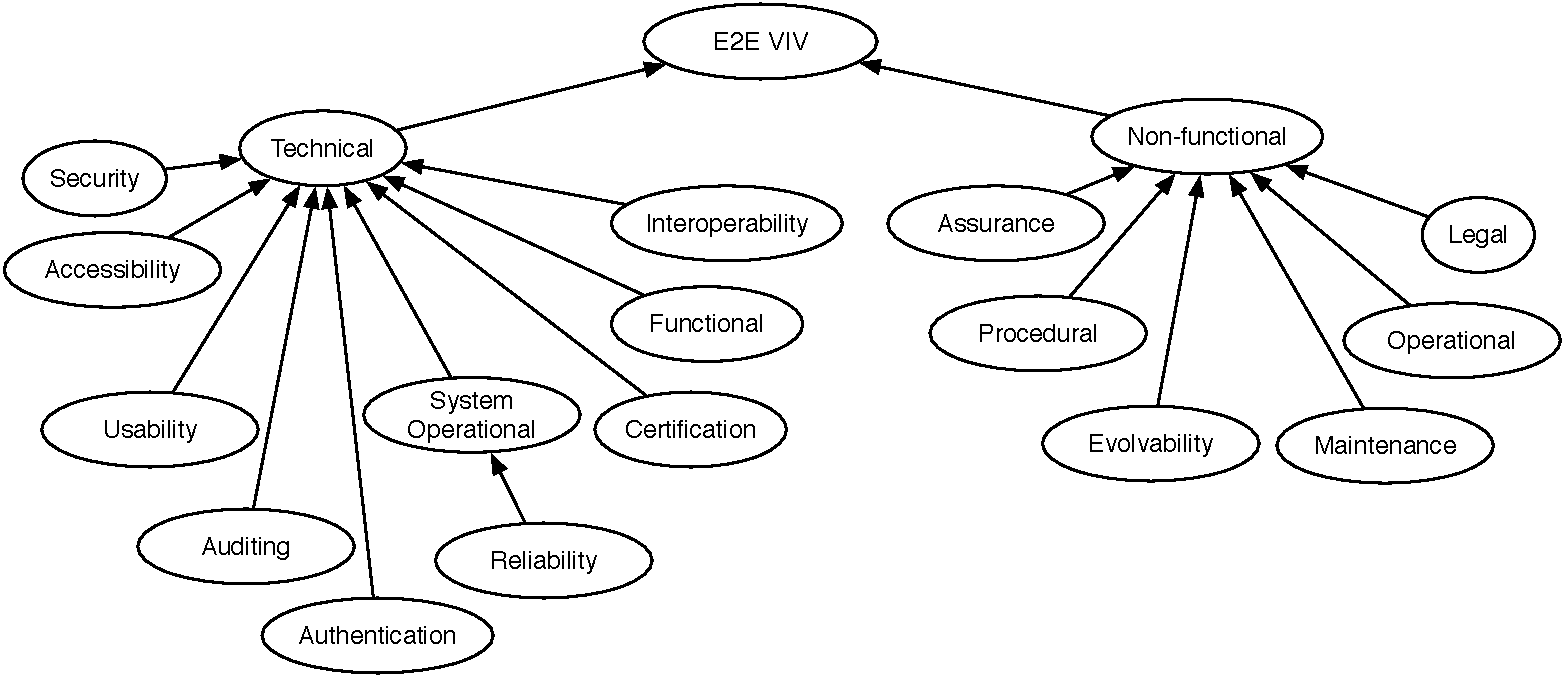
\includegraphics[width=6in]{required_properties_resources/hierarchy}
\end{center}
\caption{The hierarchy of requirements for E2E-VIV systems.}
\label{fig:e2eviv_requirements_hierarchy}
\end{figure}

The following is a high-level description of the categories and many
of the requirements within each; \autoref{appendix:bon_requirements}
contains a complete listing of all E2E-VIV system requirements
expressed in the Business Object Notation.

\section{Technical Requirements}
There are ten categories of technical requirements for E2E-VIV
systems: functional, accessibility, usability, security,
authentication, auditing, system operational, reliability,
interoperability, and certification. 

\subsection{Functional} 
\label{sec:functional}

The functional requirements of an E2E-VIV system deal primarily with
the casting and recording of ballots and associated voter records. One
important requirement is that there must be a correspondence between
the recorded ballots and the voters that are listed as having voted; a
ballot cannot be recorded without a voter casting it, and a voter
cannot be listed as having voted without casting a ballot. Similarly,
if a voter is informed by the system that her ballot has been
successfully cast, the system must correctly retain the record of her
having voted and her cast ballot information even in the event of
server failures.

Another functional requirement is the property of \emph{receipt
  freedom}: it must be impossible for a voter to prove to anybody any
information regarding how she voted her ballot, beyond what can be
mathematically deduced from the final distribution of votes. For
example, if a referendum passes with 100\% of the vote, there is no
way to hide the fact that every voter approved of the referendum;
however, if the result is mixed, it must be impossible for any
individual voter to prove how she voted.  This must be the case even
when the voter can create digital evidence of her actions by, for
example, video recording the ballot casting process or photographing a
completed ballot.

Note that there is no such E2E protocol in the literature. In order
for this requirement to be fulfilled, any protocol must allow the
voter to vote multiple times.  Yet, it must also allow it to appear
that the video-recorded vote was cast, hence its encryption must be
among those counted in a verifiable manner. Yet, this vote must not
count, and the later vote should replace it. This represents a
significant research challenge for cryptographic protocol designers.

In some elections voters are allowed to cast multiple ballots with
only the last cast ballot counting toward the final election tally,
while in others voters are prohibited from casting multiple
ballots. The system must accommodate both of these election formats,
ensuring that only the last cast ballot is counted for each voter when
multiple ballots are allowed and ensuring that each voter casts at
most one ballot otherwise.

Maintaining voter anonymity is critical, so it must be impossible
after the election to reconstruct a link between a cast ballot and any
identifying information about the voter who cast it. However, in
systems that support the casting of multiple ballots, it is important
to maintain links between voters and their ballots \emph{during} the
election to ensure that later ballots replace the correct earlier
ballots. To balance these concerns, any link between a ballot and the
voter who cast it must be irrevocably broken once it is conclusively
determined that the ballot will be counted toward the final tally.

Finally, because the voter should be able to focus on the voting
process without undue distractions or external influences, the voting
system must not display or permit the display of any advertising or
commercial logos during a voting session; the exception to this rule
is that an election jurisdiction may display its own logo to the voter
during the voting process. Along the same lines, the voting system
must not display any links to other Internet sites outside of the
voting system, except to provide help with the actual mechanics of
voting.

\subsection{Usability}

The usability of an E2E-VIV system is critical to its successful
adoption and use. Since the user experience is so important, many of
the requirements of the system have some relation to usability even
though they may be categorized under other headings. There are,
however, two requirements that are exclusively related to the
usability of the system with respect to vote casting and one general
usability requirement that applies to the system as a whole.

The first vote casting requirement is that, if a voter receives a
final vote confirmation (e.g., ``Thank you for voting!'' or a similar
notice) from the system, the ballot casting process is complete and
the system has recorded the vote.  This is the usability counterpart
to the functional requirement that ballot records and voter records
must be maintained correctly even in the event of server failures.

The second vote casting requirement is that, if a voter is uncertain
whether or not her ballot was recorded (e.g., she clicked a ``submit''
button but never got a response from the system), she must be free
to attempt to vote again.

Finally, usability testing must be performed on any E2E-VIV system
before it is deployed. The reports of the usability testing must be
made public, and the system must achieve satisfactory test results
before being deployed in a real election.

\subsection{Accessibility}

Accessibility---the property of being usable by and useful to voters
with disabilities---is one of the main goals of an E2E-VIV system. It
is closely related to usability, but there are several requirements
associated specifically with accessibility that go beyond typical
usability requirements.

Users must be involved in the design of the system to identify
accessibility constraints at each stage of the development
process. Consideration must be given to the system's compatibility
with existing technologies designed to help individuals with
disabilities; for example, the system should be developed in a way
that allows assistive input devices such as switches, eye trackers and
screen readers to be used in addition to keyboards, mice and
touchscreens. Similarly, the system's presentation of voting options
should be optimized to voters' needs by providing alternative display
fonts, audio representations, braille representations, and other
representations as appropriate.

All possible measures must be taken to ensure that the system can be
used by all voters and, if that is not possible in all circumstances,
to provide access to alternative methods of voting for those voters
who cannot use the system.

Finally, accessibility testing must be performed in addition to the
previously-mentioned mandatory usability testing. The reports of the
accessibility testing must be made public, and the system must achieve
satisfactory test results before being deployed in a real election.

\subsection{Security and Authentication}

Security and authentication are closely related and together represent
the broadest set of technical requirements, consisting of both
requirements on the E2E-VIV system itself (data storage,
communications, etc.) and requirements on the voting and counting
processes enabled by the system (voter authorization, voter privacy,
tally accuracy, etc.).

It is crucial that data integrity be ensured throughout the
system. Therefore, measures must be taken to ensure that no data can
be permanently lost in the event of a breakdown or fault affecting the
system; that the system maintains the integrity of the voters'
register, lists of candidates, ballot information, cast ballots, and
other critical information, in addition to authenticating the original
source(s) of that information and tracking provenance where
appropriate; that all data communications within the system have
associated integrity checks; that system equipment under the control
of the electoral authority is protected against influences that could
modify the election results; and that the integrity of the election
results does not depend in any way upon the security of system
equipment not under control of the electoral authority. The system
must perform regular ``health checks'' to ensure that data integrity
has been maintained, that all its components are operating in
accordance with their specifications, and that all system services are
available.

Accurate timing information is critical to security, both in terms of
providing evidence of compliance with applicable regulations and in
terms of detecting attacks on and potential breaches of the
system. The system must therefore maintain reliable synchronized time
sources, with sufficient accuracy to maintain timing data for audit
trails, election observation data, and time limits for various aspects
of the election process. It must be possible to determine, using the
timing information stored by the system, whether nominations (and, if
required, acceptance thereof by the candidate or electoral authority),
voter registration, and vote casting have occurred within the
prescribed time limits for those actions.

Authentication and authorization are also important aspects of
security. The system must ensure that each individual can be
identified uniquely, so that there is no possibility of mistaking one
individual for another. The system must also maintain the privacy of
individuals, by ensuring that all personally identifiable data is kept
confidential as far as is allowed by the legal requirements of the
electoral jurisdiction. The system must allow access to each of its
services only to authorized users; for example, only individuals who
represent the electoral authority may be allowed to load ballot
information into the system.

The authentication mechanisms used to gain access to the system must,
as far as possible, protect authentication secrets (passwords,
one-time access codes, biometrics, etc.) so that unauthorized entities
cannot acquire them. Authentication to the system may not be carried
out through third parties; that is, existing online accounts such as
those at Facebook, Google and Twitter may not be used as
authentication mechanisms. The security of the authentication
mechanism must not be affected by any potential breach of any public
or commercial database (e.g., a credit card database, the Social
Security database), and it should not be possible for an attacker to
impersonate a voter even if the entire database used for
authentication in the system is compromised. Individual authentication
secrets themselves must be changeable or revokable at any time, at the
behest of either the individual or election officials, and must be
changed for all individuals at least once in every election cycle.

With respect to the actual voting process, only eligible voters may be
allowed to cast ballots and the system must ensure that only the
appropriate number of ballots is cast by each voter. It must be
possible for a voter to verify that the system has presented her with
an authentic ballot and, in the case of remote voting, that she has a
secure connection to an official server. 

The privacy of the vote must be preserved end-to-end to the maximum
extent possible, and individual voters may not waive the privacy of
their votes. In the case of remote voting, vote privacy must be
preserved even in the presence of arbitrary malicious code on the
voter's computer (corrupted client software, key logging software or
devices, etc.). Any client software used in remote voting must not
send data to any Internet host except those associated with the E2E
VIV system or provide any information to third parties (e.g.,
Facebook, Twitter, etc.) regarding the act of voting. Any residual
information that could be used to discover a voter's choices must be
destroyed after a ballot has been cast; if a voter uses a computer
outside the control of the electoral authority to cast her vote, she
must be provided with instructions for destroying any such information
on that computer.

With respect to vote counting, the system must accurately count the
votes and the counting process must be reproducible. The system must
also maintain the availability and integrity of all information used
to generate the final tally and all information regarding the counting
process itself for as long as required. Vote tabulation must be
\emph{software independent}; it must be possible to reconstruct a
correct tally from some record even if the election system software is
compromised.

Finally, it is expected that a deployed E2E-VIV system will be an
attractive target for highly-capable adversaries that wish to
influence election results or to disrupt election processes. With this
in mind, the system must be designed and tested assuming that an
adversary has a budget of US\$10 per voter per election that can be
applied toward any critical subset of votes or voters of their
choosing; thus, an E2E-VIV system for use in a U.S. presidential
election would need to be designed and tested assuming that an
adversary has a budget of approximately US\$1,300,000,000.

The electoral authority shall have overall responsibility for
compliance with these security requirements, and such compliance shall
be assessed by independent bodies as appropriate.

\subsection{Auditing}

The ability to perform comprehensive audits of system activity is one
of the important distinguishing aspects of an E2E-VIV system as
compared to other voting systems; as a result, there are several
system requirements related specifically to auditing, in addition to
those security requirements (such as the tracking of accurate timing
information) that touch on auditing.

First, the audit system must be designed and implemented as part of
the E2E-VIV system from the beginning; it cannot be added as an
afterthought to an existing system. Audit and monitoring facilities
must be integrated into all levels of the system, from low-level
communications among individual computers to high-level interactions
with election officials. The system must keep audit logs of all
activity relevant to the conduct and outcome of the election, and
these logs must be unmodifiable once they are written and as complete
as possible without violating voter privacy.

The audit system must actively report on potential issues and threats,
rather than merely serving as a passive repository of system logs. It
must record at least the following events and actions with accurate
timing information: all voting-related information, including the
number of eligible voters and votes cast, the number of invalid votes,
count and recount results, etc.; any detected attacks on the operation
of the system or its communication infrastructure; and any system
failures, malfunctions, or other detected threats to proper system
operation. It must provide sufficient information to election
observers in real time, and after the election's conclusion, to verify
that the election is carried out in accordance with applicable
law.

The audit system must also be able to cross-check and verify the
correct operation of the voting system and the accuracy of the
election results, to detect voter fraud, and to prove that all counted
votes are legitimate and that all ballots have been counted. In
situations where the system cannot verify the legitimacy of all the
votes, it must be capable of giving an upper bound on the number of
affected ballots. If a tradeoff must be made between maintaining voter
privacy and identifying the perpetrators of fraud, the system must
resolve that tradeoff in favor of voter privacy.

In order for an E2E-VIV system to be trusted, its auditability must
extend to its own source code as well as the activities it performs
during an election. Therefore, the E2E-VIV system software, including
any official monitoring and auditing applications, must be published
in source form along with documentation, instructions for building and
running, and a digital signature as a proof of authenticity.

\subsection{System Operational}

System operational requirements ensure that the system is configured,
updated, and run in a transparent, accountable way that allows for the
other requirements to be fulfilled. One important such requirement is
that there must be official published manifests of the system used to
run any election, indicating details of the software and versions
used, dates of installation, and brief descriptions of their
functionality. Well-defined procedures must exist for both updating
the manifests to reflect changes to the installed software and
checking the installed software against the manifests to detect
tampering.

Before every election period, all equipment (including all software)
must be checked and approved in accordance with procedures devised by
the electoral authority. This check must include a check of the
software against the manifests, as well as any necessary tests to
establish that the system complies with its technical specification.

During an election period, key equipment must be located in a guarded,
secure area at all times. There must be a contingency plan for system
failures including provisions for backup and failover systems, which
must conform to the same standards and requirements as the systems
they replace. In addition, sufficient arrangements for data backup
must be in place, continuously monitored, and always available during
the election; election staff must be ready to intervene rapidly,
according to a procedure established by the electoral authority, in
the event of incidents during an election. Individuals responsible for
the voting equipment must follow established procedures to ensure that
the equipment and its use satisfy requirements.
 
To ensure accountability on the part of the electoral authority and
election system vendors, a report containing every software manifest
change and every violation of data security, system security, physical
security or control procedures must be prepared and made public by the
electoral authority within a reasonable amount of time after every
election.

\subsection{Reliability}

In order to be successfully used to conduct elections, an E2E-VIV
system must satisfy strict reliability requirements with respect to
both its behavior under normal conditions and its behavior while under
attack.

In general, the back-end (i.e., non-voter-facing) components of the
system must have a proven mean time before failure (MTBF) of at least
one week under constant peak expected load; that is, it must have been
shown in multiple actual tests of mock elections to run continuously
for at least a week at the highest expected voter participation
rate. The one week MTBF requirement applies only during normal
operation, not while the system is under attack.

In addition to the MTBF requirement, the system must also exhibit
99.9\% uptime during the election period, and must be able to recover
from any failure other than a regional natural disaster or malicious
attack in less than 10 minutes. This must be demonstrated by inducing
failures in actual mock election situations, e.g., by unexpectedly
unplugging servers or disconnecting storage devices. Redundant
failover components must be in place for all critical components of
the system in order to ensure the 10 minute maximum recovery time.

An E2E-VIV system is likely to be a tempting target for distributed
denial of service (DDoS) attacks; it must be able to continue correct
operation during a sustained DDoS attack at a specified level on any
combination of its back-end components with no more than a specified
acceptable degradation of response time to voters during the
attack. The specified attack level and acceptable degradation of
response time will vary among election types; for example, a system
running a national election must be able to resist a significantly
higher level of attack than a system running a county election. Our
initial suggestions for the thresholds for a national election are
that the system must continue operating correctly under a DDoS attack
at a level of 100 gigabits per second, with no more than a 15 second
degradation of response time.

The ability of the system to survive DDoS attacks and continue
operation while fulfilling the response time requirements must be
demonstrated in the actual network configuration to be used during the
election, and the required thresholds for these values should be
re-evaluated every election cycle to keep pace with advancement in
attack technology.

\subsection{Interoperability}
\label{sec:interoperability}

E2E-VIV systems must use open, rather than proprietary, data and
communication standards for interoperability among their various
components and services. Whenever possible, the Election Markup
Language (EML) or a similar standard ratified by an international
standards body should be used for data interchange and configuration
within the system. The standards used within the system should allow
for localization of election data in situations where such
localization is required.

The log data for the system, and documentation describing its meaning
and format, must be available for public download so that anybody can
download, inspect, and publish concerns based on the system logs. 

\subsection{Certification}

In order to provide sufficient evidence for certification of an E2E
VIV system, each functional requirement must have an associated set of
automated tests that demonstrate its fulfillment. These tests must be
runnable on demand, and their results should be unambiguous and easily
understandable.

In addition, the election protocol implemented by the system
(communication, cryptographic, etc.) must have associated formal
proofs of correctness and security to the extent possible. Note that
until recent years it was rarely possible to provide proofs of
integrity properties, hence security properties that are proven
tend to be privacy properties, but this state of affairs is evolving
rapidly in the verification community.

\section{Non-functional Requirements}

There are five categories of non-functional requirements for E2E-VIV
systems: operational, procedural, legal, assurance, and
maintenance/evolvability.

\subsection{Operational}
\label{req:operational}

The operational requirements on E2E-VIV systems deal with several
distinct issues including election and registration timing, voter
registration, candidate nominations and lists, receipt freedom, voter
assistance, and the handling of hardware and software platform issues
and election integrity violations.

Voters must be informed, in clear and simple language, of how
electronic voting will be organized and what steps a voter will need
to take in order to participate and vote electronically. Support and
guidance with respect to voting procedures must be available to all
voters. In the case of remote voting, such support and guidance must
be available through a different, widely-available communication
channel (such as a dedicated phone number) in addition to being
available via the Internet. Voters must receive clear guidance about
exactly what client configurations (i.e., hardware platforms,
operating systems, browsers, browser plugins, other applications, and
versions thereof) are required by or supported by the E2E-VIV system,
and what common components, plugins, or other software (e.g., pop-up
blockers, script blockers) may interfere with voting. In addition,
voters must receive clear guidance about configuration choices they
can make to more strongly protect their privacy; for example,
disabling cookies and browser history logging, running
privacy-protecting browser plugins, voting from temporary virtual
machines, logging out of social networks, disabling
non-election-related Internet communications, etc.

In any election carried out using an E2E-VIV system, the relevant
jurisdiction's legal provisions must provide for clear timetables
concerning all stages of the election. The period during which a vote
may be cast electronically must not begin before the public is
notified of the election; in particular, with respect to jurisdictions
that allow remote electronic voting, the voting period must be defined
and made known to the public well in advance of its start. In
jurisdictions where remote voting takes place concurrently with voting
at supervised polling stations, the time periods for remote and
supervised voting need not be identical; however, remote voting should
not be allowed after the period for supervised voting has ended.

An E2E-VIV system must have a publicly accessible voters' register
that is regularly updated. Each voter must be able to check, at a
minimum, that her information as recorded on the register is accurate,
and must be able to request corrections of any inaccurate
information. In jurisdictions where remote electronic voting takes
place concurrently with voting at supervised polling stations, the
system must be designed in a way such that it prevents any voter from
voting more than once.

On any electronic ballot, all voting options must be presented
equally; that is, there must be no distinguishing fonts, sizes,
styles, or other embellishments that could cause one or more of the
voting options to be perceived by a voter as ``preferred''. The ballot
must be free of any information about the voting
options---biographical information about candidates, interpretations
of and statements about ballot initiatives, etc.---other than
information strictly required for casting the vote or required by law
to be on the ballot (for example, candidate party affiliation is often
required to appear). The system must also avoid displaying any
messages that may influence voters' choices. Additional information
about voting options might be made available from an electronic voting
site as part of an E2E-VIV system, separate from the actual electronic
ballot; if so, such information must be presented without bias.

E2E-VIV systems are likely to be made available for testing by voters
and election officials, both before and during elections. They must
therefore indicate clearly, before the final casting of any ballot,
whether the ballot is being cast in a real election or as part of a
test. In the case of a test that occurs simultaneously with a real
election, individuals casting test ballots should subsequently be
directed to the appropriate voting channel for casting real ballots.

E2E-VIV systems must exhibit receipt freedom (mentioned previously in
the technical requirements); that is, they must not enable the voter
to possess a proof of the choices they have made in a cast
vote. Receipt freedom has two different meanings, depending upon
whether or not the voting apparatus is supervised (in a polling place)
or unsupervised (as is the case in most remote voting systems).

In a supervised environment, voting information should disappear from
the display (visual, audio or tactile, depending on accessibility
requirements) used by the voter to cast the vote as soon as the vote
has been cast. When a paper proof of an electronic vote is provided to
the voter at a polling station, the voter must not be allowed to show
it to any other person or to remove it from the polling station. Note
that the only existing protocols with receipt freedom are those that
assume a private channel with the voting system and/or a trusted
voting computer. This is not necessarily a reasonable assumption in a
remote voting scenario.

In the unsupervised setting, as discussed in
\autoref{sec:functional} above, the situation is different,
though the underlying secure goal is the same.  Even were an
adversary/coercer were to digitally record the voting process or the
voter were to record themselves with the intention of selling their
vote, it must not be possible for the adversary to irrefutably
conclude, either during the election or after the election is
certified, that the coerced/sold vote is, in fact, as recorded.

With respect to counting the votes, an E2E-VIV system must not allow
the disclosure of any vote counts until after the system has stopped
accepting electronic ballots. Tally information must not be disclosed
to the public until after the end of the voting period (including all
polling station voting). Any decoding required for the counting of the
votes shall be carried out as soon as practicable after the end of the
voting period; representatives of the electoral authority must be able
to participate in, and observers must be able to observe, the counting
process. A record of the counting process must be kept, including
timing information and identifying information for all persons
involved in the counting process. In the event of any irregularity
affecting the integrity of votes, it must be recorded that the
affected votes had their integrity violated; the effect of such
integrity violations on the election results will vary based on the
legal provisions of the involved jurisdictions.

Finally, any deployed E2E-VIV system must function correctly as an
open system, where large parts (specifically, any remote client
hardware and software) are unknown, unsecured, uncertified, and
completely out of the control of election officials. The system must
be auditable to the extent possible given this requirement, and the
conclusions drawn from the audit process should be applied in future
elections.

\subsection{Procedural}

Successful deployment of E2E-VIV systems requires certain procedures
to be followed with respect to their provisioning, certification,
maintenance, availability, and use. Because such systems are critical
pieces of public infrastructure, information about their functioning
must be publicly available and information about the specific
components of a system must be disclosed, at least to the relevant
electoral authority, as required for verification and certification
purposes. Before any such system is introduced, at appropriate
intervals after its introduction, and in particular when any changes
are made to the system, an independent body appointed by the electoral
authority must verify that the system is working correctly and that
all necessary security measures have been taken.

After introducing a system, the electoral authority must take steps to
ensure that voters undesrtand its use and have confidence in the
system; these may include outreach, practice elections, and any other
measures the electoral authority sees fit. In particular, voters must
be given an opportunity to practice any new electronic ballot casting
method before, and separately from, the casting of an electronic
ballot during a real election.

The electoral authority must take steps to ensure the reliability and
security of the E2E-VIV system; for example, guarding equipment,
providing suitable reliable power supplies, etc. All possible steps
should be taken to avoid the possibility of fraud or unauthorized
intervention during the voting process, and the electoral authority
must satisfy itself that the E2E-VIV system is genuine and operates
correctly before using it to conduct a real election. 

Only individuals appointed by the electoral authority should have
access to the central infrastructure, the servers, and the election
data, and clear rules should be established for such
appointments. Critical technical activities must be carried out by
teams of at least two people, and the composition of such teams must
be regularly changed. As far as possible, critical technical
activities should take place outside of election periods. 

Observers must be allowed to be present, to the extent permitted by
law, to observe and comment on the conduct and establishment of the
results of any election conducted using an E2E-VIV system. During an
election period, any authorized intervention affecting the system must
be carried out by a team of at least two people, be the subject of a
written report, and be monitored by representatives of the election
authority and election observers.

The system must maintain the availability, integrity, and
confidentiality of the votes. It must also keep the votes sealed until
the counting process begins. Any votes stored or communicated outside
controlled environments must be encrypted. Recounts must be possible,
and any features of the system that may influence the correctness of
the result must be verifiable. The system must also support partial or
complete re-runs of elections. 

Finally, there must be clear technical and legal procedures to be
followed in the event that voters can prove that their votes were not
received accurately or counted, or in the event that the official
election verification application does not verify that the results of
the Internet portion of the election are correct.

\subsection{Legal}

Legal requirements arise primarily from the application of existing
law to E2E-VIV systems. These include requirements on accessibility
and availability; on the counting of votes, number of votes per voter,
and anonymity of votes; and on restrictions with respect to reverse
engineering or testing of E2E-VIV systems.

To comply with accessibility and availability requirements, the voting
interface of an E2E-VIV system must be understandable and easily
usable, and registration requirements for electronic voting must not
pose an impediment to voter participation. E2E-VIV systems should be
designed, as far as is practicable, to maximize the opportunities they
provide for voters with disabilities. Unless remote electronic voting
channels are universally accessible, they must be used only as an
additional and optional means of voting beyond polling places or more
traditional remote voting methods.

The E2E-VIV system must insure that at most one electronic vote from
each voter is included in the final tally, that every vote cast
electronically is counted, and that each vote cast electronically is
counted only once. In jurisdictions where electronic and traditional
voting channels are used in the same election, there must be a secure
and reliable method to aggregate all votes, prevent multiple votes by
the same voter from being counted, and calculate correct results.

The way in which voters are guided through the process of electronic
voting should be designed to prevent their voting precipitately or
without reflection. Voters must be able to alter their choices at any
point during an electronic voting process before casting their vote,
or to stop the voting process, without their previous choices being
recorded or made available to any other person under any
circumstances. The electronic voting system must not permit any
manipulative influence to be exercised over the voter during the
voting process, must provide the voter with a means of participating
in the election without exercising a preference (e.g., by casting a
blank ballot), must indicate clearly to the voter when the voting
procedure has been completed, and must preserve voter anonymity.

There must be no legal impediments to interested parties who want to
study the E2E-VIV system. In particular, no nondisclosure agreement or
contract of any kind may be required for such download and study, or
for building, testing and publishing test results for the E2E-VIV
system.

\subsection{Assurance}

There are several assurance requirements with respect to the
implementation, documentation, and licensing of E2E-VIV
systems. First, client side software---that is, any software that is
expected to be used on a system serving as a voting terminal, whether
a supervised machine at a polling place or an unsupervised machine
belonging to a voter---must be free of known bugs on a wide range of
platform and software stack combinations. As previously discussed in
\autoref{req:operational}, the specific supported platform and
software stack combinations for the software must be clearly conveyed
to voters. The system must exhibit strong security with respect to
voter authentication, such that there is no way to automate forging or
invalidation of voter authentication credentials without compromising
the cryptographic protocols or secrets used in the system.

All aspects of the design, architecture, algorithms and documentation
for the entire Internet voting system (not just the E2EV core) should
be published and available for free download by anyone. As the system
changes, all associated documentation must be kept up to date, and no
new version of an E2E-VIV system should be certified until it has
up-to-date documentation. 

The source code, build scripts, issue tracking system, security
features, and related development information for the entire Internet
voting system---all versions, for all supported platforms---should be
made publicly available for free download and inspection, under a
license that permits anyone to download, build, instrument, and test
the system.

\subsection{Maintenance and Evolvability}

Maintenance and evolvability requirements are closely related, and
essentially stipulate that an electoral authority, or any entity
engaged by an electoral authority, must be able to change an E2E-VIV
system in response to changes in the legal or technical environment in
which it operates. 

The electoral authority must have the right and the ability to update
the election system to conform to changes in applicable law, available
technology, or threats to system integrity independent of the original
vendors of the system. The electoral authority must also have the
right and ability to patch election systems to correct flaws
discovered in the algorithms, implementation, or deployment, subject
to the documentation update requirement described above and the
procedural requirement that the system must be re-verified for correct
operation before being used to conduct a real election.
 % Dan
\iftechreport
\chapter{Crypto Specification\ifdraft{ (Joe R.) (15\%)}{}}
\label{chapter:crypto_spec}

 % Aggelos
\chapter{Architecture\ifdraft{ (Joe K./Dan) (15\%)}{}}
\label{chapter:architecture}
 % Joe K./Dan
\chapter{Rigorous Software Engineering\ifdraft{ (Joe K./Dan/Adam) (95\%)}{}}
\label{cha:rigor-softw-engin}

Sound engineering practices are the foundation for building reliable
and secure software systems. This is particularly true for critical
systems that must be trusted to perform important tasks correctly, and
where the consequences for failure threaten life, property, or
political system integrity.

The engineering of any software system can be roughly divided into
four stages: specification, implementation, verification/validation,
and maintenance. These stages are not mutually exclusive; for example,
a specification can be refined during implementation and
verification/validation can occur continuously during implementation
and maintenance.

Specification is the most important stage, particularly when building
critical systems: it informs the entire development process by
determining what must be built and what it must, and must not,
do. Even if a system works perfectly, it is impossible to provide
convincing evidence of its correctness without using and consistently
maintaining a high-quality, accurate specification throughout the
development process. Such evidence is essential for critical systems
to which we entrust our lives, money, or votes.

Implementation is the transformation, either automatic or manual
(typically some of each), of a system's specification into executable
code. The quality of an implementation is heavily influenced by
choices of programming languages, coding conventions, and supporting
tools, some of which are driven by choices made during specification.

Verification and validation are closely related, but independent,
procedures. Verification is an evaluation of whether the
implementation is a correct realization of its specification, while
validation is an evaluation of whether the implementation is
satisfactory to external stakeholders. Verification and validation are
typically carried out continuously and automatically during the
development process, using a variety of tools and techniques; the
results of verification and validation are the primary sources of
evidence for the implementation's correctness.

Maintenance includes tracking and fixing defects discovered in the
implementation, modifying the specification and implementation as
required by technical issues or feedback from external stakeholders,
and adapting the implementation to new hardware and software platforms
and new deployment environments. Maintenance is closely linked with
verification and validation, since new evidence of the system's
correctness must be provided when changes are made to either its
specification or its implementation.

This chapter introduces rigorous software engineering techniques for
these stages of the software development processes. We particularly
focus on specification, verification, and validation, since
implementation and maintenance are widely discussed throughout the
software engineering literature; however, we do describe specific
implementation and maintenance techniques that are particularly
important when developing critical systems. Finally, we recommend
specific technologies to use when constructing critical systems and
briefly discuss the current state of elections technology in light of
our recommendations.

\todo{Fix that last sentence depending on what the end of the chapter
  actually ends up looking like, and figure out what to do about the
  word ``we'' throughout.}

\section{Informal Specifications}

An \emph{informal system specification} is a human-readable
description of the system's purpose, functionality, and high-level
design. Informal specifications should be understandable not only to
the system's developers, but also to other stakeholders: clients for
whom the system is being developed, users of the system,
administrative staff who maintain the system, and auditors who
evaluate the system.

A complete informal system specification consists of a domain model, a
set of requirements and scenarios, and a set of concept
specifications.

\subsection{Domain Models}

A \emph{domain model} of a system identifies the various concepts
(also called \emph{classes} or \emph{classifiers} in some domain
modeling techniques) in the system, their attributes and roles, and
the client and inheritance relationships among them. Domain models can
be expressed in various ways, both textual and graphical. Regardless
of their form, they are essentially lists of concepts with associated
brief human-readable descriptions of themselves and their
relationships to other concepts. A good domain model provides a shared
vocabulary and gives a big picture view of the concepts involved in
the system upon which all the stakeholders can agree.

For example, the domain model for E2E-VIV systems (see
\autoref{appendix:domain_model}) includes, among many others, the
concepts ``election'', ``contest'', ``ballot question'', and
``choice''. It describes an election as ``a formal process of
selecting choices in one or more contests'', and says that a ballot
question is a specific type of contest, namely ``a decision among two
or more courses of action''. The relationship between a ballot
question and a contest is an inheritance relationship: a ballot
question \emph{is a} specific type of contest, with a certain set of
characteristics. One relationship among elections, choices, and
contests is that an election \emph{has}, or \emph{is a client of}, at
least one choice and at least one contest, because the description of
an election explicitly refers to choices and contests.

Importantly, while a good domain model comprehensively identifies and
defines the concepts and relationships in a system, it does not
otherwise constrain the realization of those concepts and
relationships or the actual behavior of the system. The description of
``ballot question'' does not specify \emph{how} a decision among two
or more courses of action is made, and the description of ``election''
does not specify \emph{how} choices in contests are selected. Such
constraints on the realization and behavior of the system are
described in general terms in requirements, scenarios, and informal
concept specifications, and are precisely expressed in formal
specifications.

\subsection{Requirements and Scenarios}

A system's \emph{requirements} are, essentially, the statements that
must be true of the system's implementation when it is
complete. Requirements are typically phrased as simple
natural-language sentences, each of which expresses a single testable
property of the system. ``The e-voting system shall maintain the
privacy of individuals.'' and ``All voter authentication secrets must
be changed at least once in every election cycle.'' are examples of
E2E-VIV requirements; the full set of requirements is described in
\autoref{chapter:required_properties}, and the informal requirements
document itself is in \autoref{appendix:bon_requirements}.

There are several different kinds of requirement, but they can be
broadly divided into two basic types: \emph{functional} and
\emph{non-functional}. Functional requirements are those that specify
how the system must behave and what outputs it must generate given
certain sets of inputs under certain conditions. For example, one
functional requirement of E2E-VIV systems is that only eligible voters
may cast ballots. Non-functional requirements are those that specify
overall characteristics of the system, such as a lower bound on its
availability or an upper bound on its cost. For example, one
non-functional requirement of E2E-VIV systems is that they must be
Open Source.

\emph{Scenarios} are descriptions of interactions among the entities
in the system, or between the system and its environment. A scenario
is typically expressed as a short paragraph describing the actions of
the entities involved, though numbered lists (to indicate a sequence
of operations) or communication diagrams (to indicate the flow of data
during a scenario) are also reasonable representations. A scenario may
also be expressed as a collection of requirements that, together,
describe the behavior of a part of the system under certain
circumstances.

It is important that requirements and scenarios describe not only the
\emph{ideal} behavior of the system, but also how the system deals
with situations that are less than ideal. System failures,
communication disruptions, data corruption, and malicious attacks of
various kinds should all be addressed in a system's requirements and
scenarios. It is not necessary to specify these at a level of detail
that provides explicit sequences of steps to recover from any given
failure or attack; rather, they can be addressed in general terms. For
example, one requirement of E2E-VIV systems that addresses system
failures is ``If service goes down for any reason other than regional
natural disaster or malicious attack, service must be restored in no
more than 10 minutes''.

As the system is built, \emph{traceability} of the requirements and
scenarios is critical. It must be possible to identify, for every
requirement and scenario, the related parts of the formal
specification and implementation, and the links among informal
specification, formal specification, and implementation need to be
kept current when any of them change. Moreover, it must be possible to
identify one or more system tests demonstrating that the system
implementation adequately addresses each requirement or scenario. This
should preferably be done automatically as part of testing and
continuous integration processes, in a way that makes it clear to
developers which, if any, requirements and scenarios remain to be
addressed.

\subsection{Concept Specifications}

A \emph{concept specification} is an informal behavioral description
of a concept in the system's domain model. Concept specifications help
to clarify what the roles and responsibilities of the concepts in the
model are with respect to the overall functionality of the system. A
typical concept specification is a set of English sentences called
\emph{queries}, \emph{commands} and \emph{constraints}, describing
respectively what information the concept possesses, what the concept
can do, and what limitations exist on its behavior. 

A query is phrased as a simple question, such as ``How many votes have
been cast?'' or ``Is this voter eligible to vote in this contest?'',
that the concept must be able to answer. Queries provide an informal
description of the data encapsulated in the concept, because the
concept must contain all the data necessary to answer any of the
queries that may be posed to it.

A command is phrased as an exclamation, such as ``Cast this vote!'' or
``Log this user out!'', describing an action that the concept must
take. This provides an informal description of the behavior
encapsulated in the concept, because the concept must be able to take
all (and only) the actions described by its commands.

Finally, a constraint is phrased as a declaration, such as ``A voter
must be eligible for this election to cast a vote.'' or ``Only users
that are logged in may be logged out.'', describing the circumstances
under which queries and commands may be issued. This provides an
informal description of the conditions under which queries and
commands may be issued to a concept. 

An informal concept specification has two main purposes: first, it
clarifies the roles, responsibilities and relationships of a concept
in the system. The process of creating informal concept specifications
may lead to the realization that some necessary concepts are missing
from the domain analysis, that some single concepts are actually
multiple related concepts that need to be described separately, or
that multiple concepts that were thought to be distinct are actually
aspects of the same concept. Second, it serves as a ``template'' for
developers implementing the concept, and---with appropriate tool
support for the formal specification and implementation
languages---can be used to automatically generate initial formal
specifications and implementation frameworks.

\section{Formal Specifications}

A \emph{formal system specification} is a machine-readable,
mathematical description of the system's functionality and design. It
is a refinement of an informal system specification, and there must be
a demonstrable and traceable correspondence between the informal and
formal system specifications. Formal specifications are meant to be
used both by the system's developers and by the various tools employed
during the development and testing process to validate the system
against its specification. They may also be used to automatically
generate partial or full implementations of system components, create
and run test suites, and generate part of the system documentation.

A complete formal system specification consists of architecture,
concept, source code, and protocol specifications; some of these, such
as the architecture specification, may be minimal for simple
systems. As we describe these types of specification, we also
introduce the verification techniques that are applicable to each.

\subsection{Architecture Specifications}

An \emph{architecture specification} is a precise description of the
system's architecture, formalizing both the relationships among the
concepts in the system and the relationships between these concepts
and the physical implementation of the system. 

Architecture specifications describe both the software architecture
and the hardware/network architecture on which the software runs. A
software architecture specification describes how many instances of
each concept exist within the system, the communication patterns among
the concepts, and any containment relationships among the concepts. It
also describes, at least at an abstract level, parts of the overall
software architecture that are external to the system under
development. For example, it may describe the relationships between
the concepts in the system, the services provided by the operating
system on which the software will run, and any external services (such
as databases or web servers) on which the software depends.

A hardware/network architecture specification describes the
relationships among the various hardware components in the
system. This includes the services provided by each component and the
network connectivity and communication patterns among them, as
discussed in \autoref{section:primary_architectural_variants}.

Some research has been done with respect to verifying software
implementations or hardware simulations against architectural
specifications~\cite{Linhares07, Abdoul08} and some tool support
exists for such verification; however, it is currently infeasible to
verify a distributed hardware and software implementation against an
architectural specification.

\subsection{Concept Specifications}

A \emph{formal concept specification} is a formal behavioral
description of a concept in the system's domain model. Formal concept
specifications are refinements of informal concept specifications, as
described in the previous section. It is possible for multiple
informal concept specifications to refine to the same formal concept
specification; for example, two informal concept specifications
``list'' and ``queue'' might both refine to the formal concept
specification ``linear data structure''.

Like informal concept specifications, formal concept specifications
have queries and commands; in formal concept specifications, these are
expressed as typed interfaces to the concept called
\emph{features}. For example, a formal specification of the
``election'' concept might refine the informal query ``How many votes
have been cast?'' with a feature of type \texttt{integer} called
\texttt{number\_of\_votes\_cast}, and the informal command ``Cast this
vote!'' with a feature of type \texttt{vote -> void} (that is, taking
a vote as a parameter and returning no result) called
\texttt{cast\_vote}. It is possible for a single query or command to
refine to multiple features of different types; for example, a ``Log
in!''  command might be implemented as two features, one taking
username and password parameters and the other taking an
authentication token parameter.

Features may be restricted, accessible only to a given concept or
group of concepts, or unrestricted, accessible to the entire
system. It is possible for a concept to have restricted features that
are not direct refinements of its informal queries and commands. For
example, the ``election'' concept might have restricted features
representing the entire database of candidates for office and ways to
update that database, but only allow unrestricted access to the
database via a query (refined from the informal specification)
requesting the candidates for a particular race.

Formal concept specifications also have constraints, expressed as
\emph{preconditions} and \emph{postconditions} on features or as
\emph{invariants}, as appropriate. Preconditions, postconditions and
invariants are part of the Design by Contract development
technique~\cite{OOSC}: a precondition is a predicate that must be true
in order to invoke a feature; a postcondition is a predicate that must
be true after a feature has been invoked; and an invariant is a
predicate that must be true at all (observable) times. For example, an
informal constraint that the number of votes cast can never be
negative could be expressed as a postcondition \texttt{Result > 0} on
the \texttt{number\_of\_votes\_cast} feature (guaranteeing that the
result of invoking the feature is always non-negative), or could be
expressed as an invariant \texttt{number\_of\_votes\_cast > 0} on the
``election'' concept as a whole.

In addition to refinements of queries, commands and constraints, each
formal concept specification also contains refinements of inheritance
and client relationships described in the domain model. Inheritance
relationships are directly stated in formal concept specifications,
and client relationships are implicitly stated through the types
assigned to the concept's features.

A formal concept specification, like an informal one, has two main
purposes. First, it expresses some of the requirements of the system
in precise mathematical terms that can be checked for various
desirable properties, such as logical consistency, before
implementation begins; this allows for early detection of a class of
possible problems with the requirements or their realizations. Second,
it can be used with automated code generation tools to create a
significant amount of the implementation and source code specification
automatically, in a provably-correct and traceable fashion.

\subsection{Source Code Specifications}

A \emph{source code specification} is an annotation integrated into,
or otherwise associated with, a piece of source code that makes formal
statements about the code's behavior. Source code specifications are
typically direct refinements of the preconditions, postconditions and
invariants from formal concept specifications, and often are the same
mathematical statements rendered in a different syntax. However,
source code specifications may also formalize aspects of the system
that are not dealt with in the formal concept specifications, such as
memory and CPU usage limits, algorithmic efficiency, fine-grain
concurrency properties, and cross-concept properties that cannot be
expressed (or are difficult to express) in individual concept
specifications, but are otherwise expressed in, e.g., non-functional
requirements.

Source code specifications are generally written in a language that is
closely related to the implementation language, and in some cases are
written in the implementation language itself. Thus, the choice of
implementation language has a significant effect on what source code
specifications can be written and how much effort it takes to write
them. With appropriate tool support, which is available for several
implementation languages of various styles, many source code
specifications can be generated automatically from formal concept
specifications. Additionally, some can be inferred by analyzing parts
of the implementation.

Source code specifications enable extended static checking
(ESC)~\cite{ESC98} tools to verify, using automated theorem proving
techniques, that implementations satisfy their formal specifications
without actually executing the code. This verification is
\emph{modular}, meaning that individual components of the
implementation are verified in isolation. For example, when verifying
the postcondition of a feature $X$ the verifier makes a number of
assumptions: first, that $X$'s precondition is satisfied when $X$ is
invoked; second, that all invariants applicable to $X$ are satisfied
when $X$ is invoked; and third, that all features invoked by $X$
behave correctly with respect to their specifications. This modularity
allows static verification to be performed continuously during system
development in an efficient, incremental fashion, providing assurance
that the completed parts of the implementation are correct and
highlighting the parts of the implementation that do not yet satisfy
their specifications.

Source code specifications can provide significant benefits at runtime
as well. Runtime assertion checking compilers can use the
specifications to generate executable code that continuously checks
for runtime violations of the specification and flags errors when such
violations occur. Automated test generators can use the specifications
to generate high-coverage unit test suites to exercise the
implementation. Runtime assertion checking and automated test
generation can significantly increase the reliability of the finished
system, and in most cases require minimal developer effort after the
specifications are written.

\subsection{Protocol Specifications}

A \emph{protocol specification} is a formal description of an
information exchange among multiple parts of a system. Each distinct
type of information exchange in the system---such as registering a
candidate or casting a vote---has an associated protocol that must be
followed. We consider only \emph{application-level protocols} that
specify what type of information is exchanged, how it is encoded, how
(and whether) it is encrypted or digitally signed, and the sequences
of interactions the involved parties perform. We assume the existence
of well-specified lower-level protocols that enable information
transmission, such as the transport protocols used to encode
information into Internet Protocol packets and the physical protocols
used to convert those packets into electrical or optical signals and
send them to remote destinations.

Application-level protocols are described, typically in terms of
communicating finite-state machines, using one of several languages
specifically devised for protocol specification. Automated tools
process these descriptions to verify that the protocols have, or
demonstrate that they do not have, various properties. These include
both security properties, such as whether an adversary can gain access
to data that is supposed to be secret or modify data without being
detected, and non-security properties, such as whether the protocol
always terminates in an acceptable state. Protocol specification
languages and tools are typically designed to specify and verify
cryptographic protocols, but can also be used to specify and verify
insecure communication protocols by simply ignoring security
properties; in the case of an E2E-VIV system, the vast majority of the
application-level protocols are cryptographic protocols and require
security property verification.

The choice of protocol specification language is almost always
independent from any other specification language choices made when
engineering a system, because of its specialized nature: specifying
and verifying the interactions of a multiparty protocol is
significantly different from specifying and verifying the behavior of
individual features or software modules. However, once a protocol is
verified, parts of its formal description can be embedded in the
source code specifications of appropriate system modules. For example,
the module that implements the receiving side of a vote casting
protocol can (and should) contain an associated formal model of the
appropriate protocol state machine and its state transformation rules;
this model can then be verified and validated in a modular fashion
alongside the rest of the source code specifications to provide
evidence that the system actually implements the verified protocol.

\section{Implementation Methodology}

Once initial informal and formal specifications are developed, the
remaining stages of the software development process can begin. In
this section we describe some best practices for software
implementation, validation and maintenance that apply not only to
critical systems, but to software systems in general. These include
testing (the primary component of validation), version control and
continuous integration, issue tracking and code review, release
management, documentation practices, and process automation. This set
of practices is not mean to be exhaustive. For example, we do not
discuss particular code standard choices or the relative merits of
various Agile development methods, as these are primarily matters of
development team preference and have little bearing on the reliability
of the resulting software. Instead, we focus on practices that are
directly relevant to building and maintaining critical systems and
generating evidence of their correctness.

\subsection{Testing}

Software testing practices are a key component of any software
engineering methodology. Even when parts of a system are formally
verified, testing can provide additional assurance that the system
satisfies its requirements, behaves as expected for particular inputs,
works correctly in diverse environments, and has sufficient
performance.

Testing serves the key functions of uncovering flaws quickly and
ensuring that previously-fixed flaws do not recur in later software
versions. It is impossible for testing to reveal all possible flaws in
any realistic program---the number of possible inputs for any such
system is so large that an exhaustive test would effectively run
forever---but tests that successfully reveal and prevent recurrences
of some flaws provide some evidence for a system's correctness.

Verification and testing should not be viewed as opposing
alternatives, but rather as complementary techniques that together
provide assurance in the developed software. It is not feasible to
exhaustively test every possible input and every possible path through
any non-trivial program, while verification offers guarantees over all
possible inputs. However, verification usually cannot scale to provide
those guarantees for entire systems; verification tools must sometimes
make simplifying assumptions about the environment in which software
runs or reason about a simplified model of the actual system. Since
testing can exercise the real system in a real environment, it can
uncover flaws that are beyond the scope or capability of verification.

Different testing practices provide complementary types of assurance;
no single testing practice is sufficient. Instead, multiple types of
testing should be used in combination on every project.

\subsubsection{Unit Testing}

\emph{Unit testing} exercises the smallest components (the ``units'')
of a program that are feasible to test. The granularity of unit tests
varies by programming language, but typically unit tests are small
enough to test the implementation within a single module, class, or
other per-file abstraction.

Unit tests are usually written to reflect the specification of the
unit under test. For example, a unit that implements a specification
of addition might have unit tests that check the associativity and
commutativity of the implementation. Most software specifications are
too abstract to translate directly into unit tests so, for a property
like associativity, developers must choose particular concrete values
to test. Unfortunately, developers might not choose the particular
values that would expose a flaw; when they fail to do so, the test
suite will succeed despite the presence of that flaw.

Developer intuition and understanding of the implementation increases
the likelihood that unit tests will exercise code containing a flaw,
but tests still cannot be exhaustive. Code coverage, the percentage of
lines of code exercised by a given test suite, is often used to
measure the effectiveness of unit tests. In practice, high code
coverage percentages have not been shown to necessarily uncover more
flaws~\cite{inozemtseva2014coverage}, however more sophisticated
coverage measures such as branch coverage are more
promising~\cite{gligoric2013comparing}.

\subsubsection{Randomized and Fuzz Testing}

Manually-written tests can only exercise a small fraction of the
potential inputs to a program. When test cases can be generated
randomly, it is much cheaper to produce a large number of test cases
that can explore a larger fraction of potential inputs.

With \emph{randomized testing}, developers specify a means for
generating the inputs to a test, and provide a function or ``oracle''
for evaluating whether the test succeeded with those inputs. These
test generators can more closely mirror specifications than tests that
use concrete values, as they can instead make assertions about all
possible values.

For example, a unit test for an addition implementation might by hand
assert that $0+0=0$, $1+0=1$, and $2^{32}+0=2^{32}$, but a random test
could assert that for all integers $x$, $x+0=x$. Unless the range of
the input is very small, a random test will not provide an exhaustive
proof of the property it expresses. It can, however, easily provide
orders of magnitude more test cases than hand-written tests, and will
usually produce test cases that a developer might not think to add
intuitively. When a higher level of assurance is required, the
specification of a random test often translates directly to a logical
formula usable by formal techniques, easing the transition to a
verified system~\cite{swierstra2012xmonad}.

In the addition example above, it is straightforward to generate
random integers and check whether the results are correct. However,
randomized testing is situational, since an oracle is not always
straightforward to develop, and even the random input generator can be
quite complicated for complex input types. For example, random testing
has successfully been used to find flaws in C compilers. The
development of the C test program generator has itself been the
subject of extensive research~\cite{yang2011finding}, and the oracles
used are primarily other C compilers.

Randomized testing is difficult for programs with complex input types
and no readily-available oracles. However, a closely related technique
called \emph{fuzz testing} is useful for such programs. A fuzz testing
tool generates random input, perhaps guided by initial suggestions; it
then passes that input to the program under test and observes the
result. If the program crashes or violates any of its internal
assertions, the fuzz tester reports the result and the input that
caused it. If the program runs successfully, the fuzz tester tries
another random input. This process is repeated continuously until it
is stopped or, in some cases, until the fuzz tester determines that it
has fully exercised the program.

Fuzz testers use a variety of techniques to generate their test input,
including pure randomness, genetic algorithms (mutating previous
inputs to generate new ones)~\cite{DeMott07}, and symbolic execution
with constraint solving (calculating new inputs to avoid repeating
execution paths that have already been
tested)~\cite{Godefroid08}. Fuzz testing has exposed many critical
security issues in widely-used software, both open-source and
proprietary.

\subsubsection{Model-Based Testing}

Another method for automatically generating test cases is
\emph{model-based testing}, where formal models of the program's
behavior can be used as test oracles, as guides for choosing test
data, or both.

Formal models of program behavior can be used as test oracles by
compiling them into the software as \emph{runtime assertion
  checks}. For example, assume the specification for some function $f$
guarantees that some condition $x$ is true when it returns. If $x$ is
ever false when $f$ returns, $f$ does not satisfy its
specification. Any good set of unit tests for $f$ should detect this
divergence, and it would certainly be straightforward to write (by
hand) a test oracle that checked the value of $x$ after executing
$f$. However, in many cases $f$'s specification can be
\emph{automatically} transformed into a set of runtime assertions,
such that (in this case) an error is always raised if $x$ is false
when $f$ returns.  Compilers that perform such transformations are
available for several programming languages and corresponding
specification languages; some widely-used examples are Java and the
Java Modeling Language (JML), C\# and Code Contracts, C and the
Executable ANSI/ISO C Specification Language (E-ACSL), and Eiffel
(with its integrated specification language).

The set of runtime assertion checks derived from a formal
specification of a module effectively becomes a test oracle for that
module; in general, more precise specifications lead to better test
oracles. For a function $f$ with such an oracle, each possible input
to $f$ defines a test, and each test is run by simply calling $f$ with
that input. A test passes if all the runtime assertion checks pass and
fails if any runtime assertion check fails. If the specification of
$f$ restricts the set of possible inputs, tests that supply invalid
input are effectively meaningless and their output is ignored.

Of course, it is impractical to call $f$ with every possible input;
however, strategies such as randomized input data generation
(discussed above) and ``interesting'' input data generation (for
example, ensuring that all boundary conditions are tested for data
types with boundaries, such as numeric types) can be used to cover the
functionality of $f$ with a reasonable number of tests. Multiple test
frameworks use these techniques to automatically generate and run
model-based tests.

Formal models of program behavior can also be used as guides for
choosing test data; for example, some tools use constraint solving
techniques on programs and their specifications to ensure that test
data satisfies input constraints on the functions under test.
Techniques such as symbolic execution---analysis of the program to
determine what inputs cause what execution paths to be taken---can
also be used to choose test data, with the goal of achieving maximal
coverage using a minimal set of test cases. 

\subsubsection{Regression Testing}

In addition to unit and integration tests written to reflect the
specifications of a system, new tests should be added whenever a
defect is uncovered and fixed. Defects tend to recur in software for a
variety of reasons. The existence of the initial defect may imply that
there is some subtlety to that particular code, raising the baseline
likelihood of defects. The fix applied to the code may have only fixed
the defect under the limited set of conditions that were observed at
the time, for example in a bug report. The fix may also have depended
on assumptions about code elsewhere in the project, and the defect
might recur once those assumptions change.

Running a \emph{regression test} for every defect in the project's
history assures us that those defects are not present in the current
software artifacts. However, for a long project, the weight of that
history can make the regression suite unfeasibly large. Many
longer-term projects therefore split their regression tests into
multiple suites: a small, quick suite to run before each code commit,
a larger suite to run every night, and sometimes a full suite that
runs over weekends or before major project milestones. Since a goal of
testing is to uncover defects as quickly as possible, running tests
less frequently is a tradeoff, and prioritizing and minimizing the
cost of testing is an area of active
research~\cite{yoo2012regression}.

\subsubsection{Integration Testing}

While unit testing and regression testing find defects in individual
modules, \emph{integration testing} finds defects in the system as a
whole. This type of testing can expose flaws in the way multiple
modules interact, measure performance of the integrated system, reveal
environmental (e.g., configuration, operating system, network)
dependencies, and simulate the overall experience of the system's
users.

The most basic integration test is simply to check that the complete
system can be successfully built. Once built, integration tests
exercise substantial functionality across multiple modules, often
simulating the actions performed by a user during an interaction with
the system and checking for expected outcomes. In this sense,
integration tests are frequently the first line of validation applied
to a system.

For example, in an E2E-VIV system, one integration test might load a
ballot, make selections, change selections, and then cast the
ballot. Another integration test might follow the same steps, but then
spoil the ballot and repeat with a new ballot. While each of these
individual steps might concern only a single module, the combination
of steps helps expose potential problems with module interactions.

In addition to simulating overall functionality, integration tests
test the suitability of the software in its intended operating
environments. This is critical for systems that are intended to work
with multiple operating systems, with or without a network, or with
specialized hardware peripherals like a ballot marking device. Making
the environmental assumptions explicit in integration tests also helps
prevent defects from arising due to unstated assumptions. For example,
a developer may inadvertently write software that depends on features
that are unavailable in the deployed environment. It is
counterproductive and often infeasible to develop in the deployed
environment, which may not even be capable of running development
tools; therefore, the integration tests must accurately recreate that
environment.

\subsection{Version Control}

A \emph{version control system} (VCS) manages changes between the
versions of a project as it evolves during the course of
development. Revision control is the preferred way to share software
artifacts across a team, but all software projects, even those
developed by teams as small as one person should use a VCS.

In general, a developer uses the VCS first to ``check out'' the files
comprising a project into her ``working copy''. Then, after making
changes to those files, the developer ``checks in'' or ``commits'' the
changes to the VCS. After committing, those changes are available for
other developers to integrate into their working copies.

When different sets of changes have been made by multiple developers,
the VCS can merge those changes either automatically or by using
developer input to ensure the project remains consistent. The ability
to merge changes is critical for teams of developers who work
concurrently on a single project, and is the reason that file sharing
tools like Dropbox or Google Drive are an inadequate substitute for a
VCS.

Version control is particularly important for projects, such as
critical systems, where the development process must be auditable. An
entry to a project log is created every time a developer commits their
work. Any file in the project can be inspected to show its provenance,
even down to the level of which line was committed by which developer
on what date. Some VCS tools also allow for commits to be
cryptographically signed, offering assurance that, for example, the
changes have been audited by a trusted authority before being
integrated into the project~\cite{chacon2014pro}.

Moving from simple file storage to a VCS is a tremendous improvement
for development, but poor use of a VCS can negate many of the
potential benefits. For example, the log built from the commits of
developers is of less use to auditors if the changes in each commit
are not clearly associated with a particular new feature or bug
fix. Likewise, if developers commit changes that cause the system to
function incorrectly, other developers' productivity suffers and it
becomes more difficult later to isolate the commit that introduced a
bug. Each VCS supports multiple workflow practices that should be
adopted in order to limit these problems and get the most benefit from
VCS use~\cite{atlassianworkflow,pilato2008version}.

\subsection{Continuous Integration}

The expense of fixing software defects increases over time as other
parts of the software evolve around those defects. When a defect is
new, developers have not had a chance to write other code that depends
on the defective code. Once such dependencies exist, a fix for a
single defect can have consequences that ripple outward across the
entire project, making the fix much more expensive. The cheapest way
to fix a defect, then, is to discover it as quickly as possible.

\emph{Continuous integration} (CI) facilitates this by discovering
defects as part of a regular, automatic process that is not dependent
on due diligence of individual developers. CI interleaves the quality
control process into the development process, rather than leaving it
as a separate phase for the end of a project after development has
finished.

CI tools automatically build and test the latest version of the
software in the VCS system on a regular basis, such as every night or
after every VCS commit. Because the software is built from the VCS, it
is important for developers to frequently commit their work to the
VCS. The VCS integration ensures the tests are always run on the
canonical version of the software, and that any discovered defect can
be linked to a particular version in the VCS system. Isolating the
failing version focuses the efforts of developers on the set of
changes introduced in that version, often saving considerable time.

CI systems substantially replace manual effort and the risk of
mistakes when releasing software. Since the CI system builds the
project on a nightly basis, it can post the artifacts of those builds
for users and testers to quickly adopt. When an official release like
``Version 1.0'' is ready, developers can simply run the CI system to
produce the relevant artifacts. Because the same system is responsible
for both the continuous testing and validation of the system and the
creation of the final release, it is less likely that the final
release will have defects that would have been caught through earlier
testing.

\subsection{Configuration Management}

Complex software systems may depend on many components outside their
own implementations, including database servers, application servers,
web servers, authentication systems, etc. They may also need to run on
several different target platforms with different operating systems
and capabilities, or on multiple commercial cloud infrastructures with
different deployment and management processes.

\emph{Configuration management} is the tracking of dependencies and
deployment characteristics for a system, and is typically automated by
multiple tools. A \emph{build automation tool} handles dependency
tracking for building and packaging the software, and is used both by
developers and by the continuous integration system. A
\emph{deployment automation tool} handles the setup and configuration
of the (already built) software for a particular execution
environment, such as an operating system/platform combination or a
specific set of nodes at a specific cloud provider, including the
configuration of the individual machines on which the software will
run.

Configuration management saves significant manual effort and greatly
reduce the risks of mistakes when building and deploying software, and
should be used in all projects that have external dependencies or
target multiple deployment platforms.

\subsection{Software Product Lines}

Developing software that has to be changed in many ways for different
target audiences has historically been a nightmare.  Each different
version of such a piece software is called a \emph{variant}, and the
decision points in the software or its build system that derive
variants are called \emph{variation points}. This style of software
development is called \emph{software product lines}
(SPL)~\cite{czarnecki2005model,northrop2001software,clements2002software}.

Traditionally, one would develop such software with programming
languages that have either (a)~support for conditional compilation,
usually in the form of C-like \texttt{\#ifdef}s or Lisp-like macros,
or (b) inheritance, using sub-typing and sub-classing as a means of
selecting variants. Using the development process to achieve the same
goal typically results in a large tree of branches in a VCS, where
each branch is a (mostly) separately maintained variant.

These traditional styles of software development, without additional
supporting technology, have been shown to be unfit for this
purpose~\cite{linden2007software,kastner2008granularity,chen2009variability}.
The resulting software is typically an impenetrable mess that is
extremely difficult to maintain.

An alternative way of developing SPLs is to specify variants by
declarative means.  The academic literature highlights three good
solutions to this problem: a specification technique called
\emph{feature models}~\cite{FMs}; expressing variants using a
specification language in the context of model-driven development
(MDD) (e.g., Clafer~\cite{Clafer} or the OMG's Common Variability
Language (CVL)~\cite{CVL}); and embedded domain specific languages
(EDSLs)~\cite{EDSL}.

Product support for feature modeling and CVL is in its infancy, but is
rapidly evolving as the industry demands better support for developing
SPL-based software
systems~\cite{bosch2002maturity,bockle2004calculating}.

\subsection{Issue Tracking}

During much of the software development and maintenance process, teams
add features and fix bugs. An issue tracking system maintains records
about each new feature, each reported bug, and other discrete
development tasks from their creation to their implementation, review,
testing, and integration. Issues can be organized by metadata such as
assignee, project milestone, priority, and task type. Issue trackers
are essentially to-do lists with additional structure, specialized to
support effective software engineering.

These issues and their metadata give team members an overview of the
status and health of the project. For example, the issue tracker may
automatically require a code review step before an issue can be
resolved. Issue trackers help teams make fewer mistakes when following
best-practice software engineering workflows.

Team members can annotate issues with comments or attach supplementary
documents, creating a record of design decisions and thought
processes. This information is invaluable when investigating future
bugs or making subsequent changes to a design, and is often lost when
such discussions take place out-of-band and lose their associations
with the tasks that motivated them.

Most issue trackers integrate with VCS in order to associate issues
with source code changes. Combined with the design discussions
captured in issue comments and attachments, this enhances the ability
of the team to understand and maintain the project in the future.

When issue trackers are public they can also serve as a first point of
contact for users, providing insight into the evolution of the system
and a well-defined process for reporting system issues. In projects
with short development timelines, it is critical to incorporate
feedback into development as quickly as possible. Giving users or
front-line support staff the power to create issues directly makes the
feedback loop very small.

Public issue trackers also reduce duplicated effort by both users and
developers. If a system has a problem, that problem will likely become
apparent to multiple users; duplicate reports are less likely if users
can check the issue tracker for other reports of similar problems. The
development team can then triage issues by importance and urgency,
discuss potential solutions, assign developers to implement those
solutions, and finally make sure the problems are resolved and notify
the users who originally reported the problems.

\subsection{Code Review}

Code review practices involve examining the results of the software
development process to find defects, identify potential improvements,
and increase understanding of the software throughout the engineering
team. Reviews are also an opportunity to ensure that organizational
code style standards are met and that the code and its documentation
are easily understandable. This process, like discovering defects
during testing and investigating issue reports, feeds back into an
interative development process to improve the quality of the final
product.

Code review can be a manual process at varying levels of rigor. On the
formal end, processes like Fagan inspection require a line-by-line
inspection by many developers in an extended meeting and catch a high
percentage of defects~\cite{fagan2002design}. On the lightweight end,
code review occurs implicitly during pair programming and can take
place informally via a developer-led walkthrough or an email to
colleagues requesting feedback. Formal inspections are more costly
than informal reviews, but may be more suitable for projects that
require concrete audit trails for accountability. Lightweight methods,
particularly pair programming, can find similar proportions of defects
for lower cost~\cite{tomayko2002comparison} and have other positive
effects such as higher developer job satisfaction and improved team
dynamics~\cite{cockburn2000costs}.

Automated tools complement any form of manual code review. Lightweight
static analysis tools and code ``lint'' tools can help developers
avoid common coding mistakes and adhere to organizational style
standards. Very lightweight static tools can be run by individual
developers before committing their work to the VCS, and longer-running
analyses can be part of the continuous integration and testing
process. Such analyses are not substitutes for formal verification or
testing, however, as they typically are meant to discover small-scale
defects and help developers avoid common pitfalls rather than to
validate overall properties about the correctness of a system.

\subsection{Release Management and Lifecycle}

\emph{Release management} is the transformation of a set of software
artifacts into a finished product that can be used in its intended
environment. Release management is primarily focused on the smooth
integration of the different aspects of the project and on adhering to
practices that make releases repeatable, reliable, and auditable.

Release management and VCS workflows are tightly connected. For
example, in the Git Flow model~\cite{atlassianworkflow}, release
management would include creating a new release branch, imposing a
feature freeze (no new features, only bug fixes) on that branch, and
eventually tagging that branch upon release and merging it back into
the main development branch.

For a project that delivers software as a service on a web server,
release management would include deploying the software to production
servers. For software delivered as a binary download or CD, release
management would include cryptographically signing and distributing
the binary. In both of these cases, a release manager serves as the
final line of quality assurance before the software is used in its
intended environment, and must be fluent enough with all aspects of
the project and its processes to release software only once the
processes have been faithfully executed.

\subsection{Testable Documentation}

Documentation of the design, implementation, and use of a software
system is a standard requirement in software engineering
methodologies. However, when a system is under development and rapidly
changing, documentation can lag behind and fall out of step with the
latest version of the software, leading to errors and confusion.

Where possible, documentation should be machine-testable (or even
machine-generated) and integrated with the VCS rather than being a set
of static resources maintained independently of the software. Testable
and generated documentation is far less likely to become inconsistent with
the software it describes, because any such inconsistencies will be
detected during testing.

The form of testable documentation varies depending on the granularity
of the documentation and the underlying technologies used by the
project. For example, Business Object Notation
(BON)~\cite{walden1995seamless} can be used as analyzable
documentation at the specification, design, and architecture level.

At the level of code modules and interfaces, documentation should be
concretely executable like the ``doctest'' features available for
specification languages like JML (using its \texttt{examples} pragma)
and programming languages like Python and
Haskell~\cite{python3doctest}. Documentation in this style contains
short examples that illustrate the expected use of a system and its
expected response, for example in Python:

\begin{lstlisting}[language=Python]
"""
This is the fibonacci module. It provides the function fib which
returns the nth fibonacci number, where n >= 0.

>>> fib(0)
0
>>> fib(10)
55
>>> fib(-1)
Traceback (most recent call last):
    ...
ValueError: n must be >= 0
"""
\end{lstlisting}

Executable tests should supplement, not replace, traditional prose
documentation. Since they are essentially a form of unit test, they
suffer from the same limitations. They typically only exercise a
handful of concrete values, and cannot test non-functional properties
like expected performance or thread safety.

\subsection{Reproducibility and Automation}

A team can implement many of the techniques in this section
manually. Tests can be run by hand on developers' machines, code can
be sent out for review by email, issues can be tracked on a mailing
list, and a release manager can build and package release artifacts by
hand for each supported platform. However, each time a step in a
process must be manually performed, the probability of human error
increases and reproducing steps for later quality assurance and
troubleshooting becomes harder.

A manual operator might skip a step or perform a step out of order,
for example running the test suite before integrating the latest
changes from the VCS. The operator might also introduce new steps that
seem necessary and obvious, but unless recorded will make it very
difficult to reproduce or audit the process in the future. Finally,
manual execution of a process, even if done correctly, takes much
longer than automated execution.

To prevent errors, improve reproducibility, and make development more
efficient, processes should be automated as much as possible. The
techniques described in this section all support automation and
reproducibility or can themselves be automated to a degree, but some
play key roles.

\paragraph{Version Control}

The version control system is a linchpin of automation. The versions
it manages are the starting point for automated and reproducible
continuous integration, testing, and software releases. The VCS can
itself trigger automated processes; for example, it could trigger a
run of an automated test suite after every commit.

Any automated process should be run in the context of a particular VCS
version, and any artifacts produced by these processes should refer to
this version. For example, if software has a built-in bug reporting
feature, those reports should automatically include the version at the
time the software was built. This allows engineers to easily reproduce
the exact circumstances where a user discovered a defect.

Version control can only improve reproducibility when all relevant
inputs to a process are managed in the VCS. For example, a software
build process that depends on a configuration file in the user's home
directory would not be reproducible on a different computer without
that home directory.

\paragraph{Testing}

Manual testing can play an important role when evaluating a system,
but any realistic system requires more tests than are feasible to
perform manually. Even if the contents of a test suite are automatic,
if that test suite is only run manually it will often be skipped,
particularly when it takes a long time to run. Automating both the
tests themselves and the running of those tests ensures that they will
be run on a consistent basis, and that the results will be
reproducible and traceable to a particular version.

\paragraph{Continuous Integration}

Continuous integration is another linchpin of project
automation. Since CI tools are designed to automatically run on a
regular basis and offer integration with the VCS, other processes are
usually automated by using these tools. For example, after building
the integrated software, a CI tool should run the test suite and
archive the built artifacts for subsequent release management.

\paragraph{Configuration Management}

Configuration management is another area where automation is
critical. Tracking the software's dependencies and handling the
details of its deployment on various platforms should be left to
automated build and deployment automation tools to the extent
possible, and these tools should be run frequently. Typically,
configuration management tools are used by the continuous integration
system in addition to being used in release management.

\paragraph{Release Management}

No process has as many moving parts or cross-project concerns as
release management, making manual release management extremely
error-prone. The entire process, from checking out a version from the
VCS to deploying the final release artifacts, should be as automatic
as possible. The manual intervention should amount to simply deciding
which version to release and checking before the final release that
the automated process performed as expected.

Because automation is inexpensive when using continuous integration
and configuration management, it is a good practice to have those
tools perform parts of the release management process on a regular
basis, even when software is not ready for a release. If the process
of producing a release is the same as performing an ordinary nightly
build and test, it is less likely that problems will arise only at the
release stage when it is much more costly to address those problems.

\section{Technology Recommendations}
\label{sec:technologies}

Here, we provide some recommendations about specific technologies
that, at present, are well suited (and in some cases, \emph{not} well
suited) to performing rigorous software engineering of the type we
have described. These recommendations are based on experience applying
these methods over the last 15+ years, but they are not meant to be a
rigid set of rules or to unconditionally exclude technologies not
mentioned here. The landscape of software development languages and
tools is constantly changing; new languages and tools appear, while
old languages and tools disappear, are marginalized, or evolve in
possibly surprising ways.

\subsection{Domain Modeling}

For domain modeling, we recommend the Business Object Notation
(BON)~\cite{walden1995seamless} and Extended Business Object Notation
(EBON. BON is both a language and a design/refinement method
encompassing informal domain analysis and modeling, formal modeling,
and implementation-independent high- and medium-level
specification. BON has a well-defined semantics, is easy to learn and
write (especially the informal models, which are effectively
collections of simple English sentences), and has equally-expressive
textual and graphical notations. BON was originally developed for use
with the Eiffel programming language and is well-supported by the
EiffelStudio tool suite; however, it can be used with other
specification and implementation languages. EBON adds additional
\emph{semantic properties} to BON, allowing BON to express properties
relating to domains such as concurrency, ownership, responsibility,
bug tracking, literate programming, and version control.

We recommend BON over the Unified Modeling Language (UML), the de
facto standard for modeling in the software industry, for several
reasons. First, BON's equivalently expressive textual and graphical
notations are easy to work with and manipulate. UML supports only a
graphical notation, though there is also an unsupported official
``Human-Usable Textual Notation''~\cite{HUTN}; it was last updated in
2004, reflects only the version of UML that was current at the time,
and is not as expressive as the graphical notation. Tool support
currently exists for at least a dozen different and
mutually-incompatible textual UML dialects, none of which are as
expressive as the UML graphical notation and most of which have
significant readability issues.

Second, BON's semantics are an integral part of the language and
method and are easily understandable. By comparison, UML effectively
has no semantics; the Object Constraint Language (OCL)---the
specification language typically associated with UML models---is a
very complex expression language, and is not an integral part of UML.

Third, BON explicitly supports (and encourages) \emph{seamlessness}
and \emph{reversibility}. Seamlessness is the property that allows a
BON model to be smoothly (and, in many cases, completely
automatically) refined to lower-level specification languages, and
further to executable implementations. Reversibility is the property
that allows consistency to be maintained between the BON model, which
is an important part of the system documentation, and the resulting
implementation---when the implementation is changed, that change can
be (again, often completely automatically) propagated back up to the
BON model. Seamlessness and reversibility are both useful properties
for ensuring that the final software product accurately reflects the
original domain analysis and architecture design.

Fourth, BON supports high-level domain modeling using natural
language, making it easy to communicate models not only among software
developers but also with other stakeholders in the development
process. The BON representation of the E2E-VIV requirements in
\autoref{appendix:bon_requirements} consists almost entirely of simple
English sentences; it is therefore far more accessible to a wide
audience than an equivalent set of UML diagrams would be.

Finally, BON is \emph{simple}. Its specification is a fraction of the
size of the UML specification, and its graphical representation is
significantly less complex. For example, arrows in BON diagrams only
have two possible appearances (a single or double line, with a single
filled arrowhead) as compared to UML's proliferation of arrow types
(solid and dashed lines, filled and empty arrowheads, diamonds, and
circles, and additional connection markings). 

While we recommend BON based on our experience, it is not the only
reasonable choice for domain analysis in a rigorous software
engineering context. The Vienna Development Method (VDM)~\cite{VDM},
Z~\cite{Zed}, the B Method~\cite{BMethod}, and the Rigorous Approach
to Industrial Software Engineering (RAISE)~\cite{RAISE} are all
well-established domain analysis methods with textual representations,
well-defined semantics, and tool support.

\subsection{Formal Specification}

In addition to its use for domain modeling, BON can also be used as an
architecture specification and concept specification language and we
recommend its use as such. Once written, BON specifications can be
refined further into architectural specification languages for
expressing detailed architectural properties, source code
specification languages for integration with particular implementation
languages, and protocol specification languages for formalizing
interactions within the system.

UML is the most commonly used tool for architecture specification, but
is not well suited to rigorous software engineering because it lacks
semantics. We recommend using BON for high-level architecture
specification and a dedicated architecture specification language,
such as the SAE Architecture Analysis and Design Language
(AADL)~\cite{AADL} or the OMG Systems Modeling Language
(SysML)~\cite{SysML}, for low-level architecture
specification. Several tools support the creation and manipulation of
AADL and SysML specifications and automatic generation of code from
architectural models; some tools, like
OSATE2-Ocarina~\cite{OSATE2-Ocarina} for AADL, also support automated
verification.

Programming languages for which there is an obvious best choice of
source code specification language include Java
(JML~\cite{JMLReferenceManual}), C\# (Code
Contracts~\cite{CodeContracts}), and C (ACSL~\cite{ACSL}). Some
implementation languages, such as SPARK~\cite{SPARK2014} (a dialect of
Ada) and Eiffel, have integrated specification languages. These
specification languages all have several features that we consider
essential for efficient and effective use: straightforward syntax and
semantics, integration with widely-used software development
environments, and tool support for performing analysis and
verification. In the case of JML and Eiffel, tool support is also
available for automated reversible refinement from BON.

In any given project, different parts of the architecture may be
implemented in different languages. For example, it might be
appropriate to implement some computation-intensive parts of a design
in a language like C while implementing the rest of the design in a
language like Java or C\#. Thus, multiple source code specification
languages may be used in a single project, though we recommend that
high level specifications be written in a single language to the
extent possible.

There are also several language-neutral specification languages and
associated development tools, such as Alloy~\cite{Alloy},
Coq~\cite{Coq}, Event-B~\cite{Abrial10}, VDM~\cite{VDM}, and
Z~\cite{Zed}, which themselves support refinement to various
implementation languages. Most have associated tools for
\emph{model-based synthesis}, the process of automatically
transforming formal models into conforming executable
implementations. These languages and tools can be used effectively,
either by themselves or alongside other specification languages, in a
rigorous software engineering process; they are especially useful for
specifying, verifying, and automatically generating small, critical
system components.

Finally, any of several protocol specification languages can be used
to specify interaction protocols within the system. These include
the High-Level Protocol Specification Language (HLSPL) used by
Avispa~\cite{Avispa}, typed $\pi$-calculus as used by
ProVerif~\cite{ProVerif} and CryptoVerif~\cite{CryptoVerif},
Casper~\cite{Casper}, EasyCrypt~\cite{EasyCrypt}, and Scyther Protocol
Description Language (SPDL)~\cite{Scyther}. Each language is directly
tied to a protocol verification tool, and each tool has its own
strengths and weaknesses with respect to verifying different types of
protocol; thus, the choice of tool for verifying a given protocol
dictates the choice of language for specifying that protocol (or
vice-versa), and it may be appropriate to use different tools for
different protocols within the system.

\subsection{Implementation Language}

The choice of implementation language is clearly important, and there
are many possible choices; hundreds (possibly thousands) of
programming languages exist and dozens of those are actually viable,
with widespread adoption, tool support, and support communities. In
most cases, language choice determines programming style: for example,
Eiffel imposes an pure object-oriented style while Haskell imposes a
pure functional style. Language choice also determines the set of
existing functionality, in the form of standard libraries accompanying
the language or well-established external libraries available for use
with the language, on which developers can rely while building the
implementation. 

Implementation languages are distinguished by different styles,
different methods for error handling, different security guarantees,
and different ways in which programmers can make mistakes (both minor
and catastrophic). For rigorous software engineering, we generally
recommend languages with strong type systems that actively prevent
programmers from making any of a large class of errors. We also
recommend languages that automatically handle memory allocation and
deallocation, which prevents another large class of errors and many
potential security issues. Finally, we recommend languages that either
have good specification and verification tool support or are designed
explicitly for the implementation of high-assurance software. It is
certainly possible to implement reliable software in languages that do
not have all these features---for example, code can be written in a
safe subset of C, specified with ACSL, and verified with various
tools---but it is significantly more difficult to do so.

The nine implementation languages we currently recommend for rigorous
software engineering are (in alphabetical order) C (a safe subset such
as C$_{0}$~\cite{C0} or the C dialect supported by the Verified
Software Toolchain~\cite{VST}), C\# (excluding unsafe code), Eiffel,
Erlang, Gallina (the executable specification language for the Coq
proof assistant~\cite{Coq}), Haskell, Java, OCaml, and SPARK. No
single implementation language is ideal for every project, and it is
often appropriate to use multiple languages in the same project. For
example, it would be reasonable to write the computational core of a
voting system in a pure functional language like Haskell and the
voter-facing user interface components in an object-oriented language
like Java.

\subsection{Static Analysis}

Static analysis tools process the system's source code and
specifications to provide information about the system without
executing the code.  There are many forms of static analysis, ranging
from simple syntactic checks to full functional verification. The
following set of recommendations is not exhaustive, and in particular
does not discuss specific tools covering all the recommended types of
static analysis for all the recommended programming languages; many
useful static analysis tools that can be effectively deployed in a
rigorous software engineering process are not mentioned here.

At least one static analysis tool should be used to enforce some set
of code style and formatting guidelines, so that the implementation's
code base is consistently readable. Examples of tools that enforce
such guidelines are Checkstyle~\cite{Checkstyle} for Java and
StyleCop~\cite{StyleCop} for C\#. The style enforcement tool(s) should
be run automatically and frequently, either within each developer's
environment (for example, a Checkstyle plugin can run Checkstyle every
time a file is saved in any of the commonly-used Java IDEs) or as part
of the version control or continuous integration processes.

Static analysis tools should also be used to detect ``code smells''
and other problematic aspects of the implementation. The presence of
significant amounts of duplicate code in multiple locations in the
implementation and the excessive use of numeric literals that should
be declared as symbolic constants are examples of code smells; other
problematic aspects might (depending on the implementation language)
include memory leaks, buffer overflows, and concurrency problems.
Static analysis tools that can detect these issues include
FindBugs~\cite{FindBugs} and PMD~\cite{PMD} for Java,
ReSharper~\cite{ReSharper} for C\#, Eiffel
Inspector~\cite{EiffelInspector}, and SPARK Pro~\cite{SPARKPro}.

Finally, static analysis tools should be used to verify protocol
specifications and source code specifications. As previously
mentioned, the choice of tool for verifying protocol specifications is
dictated by the choice of protocol specification language. Source code
specifications can be verified with extended static checking tools,
such as OpenJML~\cite{OpenJML} for Java with JML specifications,
Frama-C~\cite{Frama-C} for C with ACSL specifications, and SPARK
Pro. In addition, source code can be proven equivalent to a reference
implementation or to a formal model using tools like the Software
Analysis Workbench (SAW)~\cite{SAW}; this type of analysis is
particularly useful when verifying the correctness of cryptographic
algorithms, which are pervasive in E2E-VIV systems.

\subsection{Dynamic Analysis}

Dynamic analysis tools monitor a running system to measure aspects of
its operation and detect undesirable behavior. There are many
different forms of dynamic analysis and many dynamic analysis tools;
like the static analysis recommendations above, the following set of
recommendations is not meant to be exhaustive.

One important form of dynamic analysis that we strongly recommend
using when possible is runtime assertion checking (RAC), previously
mentioned in associated with model-based testing. RAC compiles runtime
checks for specification conformance into the implementation, which
ensures that any runtime violations of the source code specifications
will be detected and reported. OpenJML for Java, Code Contracts for
C\#, SPARK 2014, and Eiffel all support RAC compilation with their
associated specification languages.

Another form of dynamic analysis that can be useful is
\emph{specification inference}. Tools like Daikon~\cite{Ernst2007},
which works on Java and C\# programs, can infer likely specifications
(particularly invariants) that may have been missed during the
specification refinement process. If these inferred specifications are
valid, and are added to the source code specifications, they can
assist ESC tools in verification and provide additional runtime
checks; in some cases, the additional specifications can allow ESC
tools to verify parts of the implementation that they otherwise could
not.

\emph{Coverage analysis} is another useful form of dynamic analysis,
particularly when used in conjunction with automated testing. Coverage
analysis tools, such as EMMA~\cite{EMMA} for Java,
OpenCover~\cite{OpenCover} for C\#, and
GNATcoverage~\cite{GNATcoverage} for SPARK, can provide information
about ``how much'' of the code was executed during a particular
run. ``How much'' can be expressed using several different metrics,
including \emph{statement coverage} (the percentage of the source
statements actually executed), \emph{branch coverage} (the percentage
of the program branches that were taken during the execution), and
\emph{path coverage} (the percentage of possible execution paths that
were taken during the execution). When used in conjunction with
automated testing these coverage metrics can give a rough idea of test
suite quality; for example, a test suite that does not exercise the
entirety of the system by at least one metric is clearly not as good
as a test suite that exercises the entirety of the system by all
coverage metrics. 

Dynamic analysis can also be used to detect issues related to memory
(leaks, corruption), concurrency (deadlock, spinning, data races),
resource allocation (unclosed sockets and files), and security (buffer
overflows and other vulnerabilities). Some of these issues are already
mitigated by the languages and other forms of analysis we
recommend---for example, none of the languages we recommend allow
programs to be vulnerable to buffer overflow attacks in the same way
that traditional C and C++ programs can be---but it is useful to run
dynamic analysis tools to detect the ones that are not. There are too
many such tools, of too many types, to list here.

Finally, dynamic analysis can be used to \emph{profile} the executable
code, monitoring it to determine which parts are executed most
frequently and to find performance bottlenecks. This allows developers
to gather empirical evidence for use in comparing multiple
implementation choices (e.g., what data structure variant to use for a
particular part of the system's data model), rather than blindly
guessing at the consequences of implementation decisions. It can also
help to direct optimization efforts when tuning the system for
performance late in the development process. All the languages we
recommend have associated profiling tools, many of which are
integrated into their respective development environments.

\subsection{Model Checking}

Model checkers attempt to determine whether a formal model of a
software system fulfills some specification, such as a requirement
that a concurrent system must not deadlock. If a model checker
determines that a model fulfills a specification, then we can conclude
that an implementation fulfills the specification if we can prove that
the implementation's behavior conforms to the model. Many of the
protocol verification tools mentioned previously use model checking
techniques.

The most widely-used model checking languages/tools are
Alloy~\cite{Alloy}, PVS~\cite{PVS}, Spin~\cite{Spin}, and
UPPAAL~\cite{UPPAAL}. Developers can write models in these languages
by hand, but it is more efficient to automatically \emph{extract}
models from existing implementation code; this guarantees that
properties proved about the model hold for the implementation. Model
extraction is supported for a number of implementation languages,

Model checking requires an exhaustive search of the model's reachable
states to determine whether any violate the specification. There are
several ways to reduce the complexity of this search, such as by
exploring multiple states with simultaneously in a symbolic fashion,
but model checking remains intractable for large software systems. We
therefore recommend that model checking be used sparingly, for only
the most critical subsystems, and that it be used primarily for
protocol verification.

\subsection{Version Control}

We recommend using either Git or Mercurial for version control. Both
are current-generation distributed version control systems, supporting
various models of collaboration, and both are well-supported. Both
also have associated services---including GitHub~\cite{GitHub} for
Git, BitBucket~\cite{BitBucket} for Mercurial, and
SourceForge~\cite{SourceForge} for either one---that provide
repository hosting, issue tracking, web hosting, and wiki
functionality. Git is currently the more popular of the two by a
significant margin, but both are good options for new projects and the
choice between them is mainly one of developer preference.

We recommend against using older, centralized version control systems
such as Subversion and CVS. In general, their mechanisms for handling
concurrent development and maintenance of multiple versions of
software are significantly more awkward than those of the
current-generation systems, and the single synchronization point
inherent in their centralized architectures makes it more difficult
for developers to work offline.

\subsection{Issue Tracking}

Many good issue tracking tools are available. If the version control
repository is hosted by one of the well-known hosting services
(GitHub, BitBucket, SourceForge), the obvious choice is to use the
issue tracker integrated with that service. Otherwise, there are
several proprietary and open-source choices for either cloud hosted or
locally installed issue tracking.

Atlassian's JIRA~\cite{JIRA}, JetBrains's YouTrack~\cite{YouTrack},
and Fog Creek Software's FogBugz~\cite{FogBugz} are all hosted issue
trackers that integrate with both Git and Mercurial repositories. JIRA
and YouTrack are also offered as standalone commercial products that
can be installed and maintained locally. All three have roughly
equivalent capabilities and the choice among them, like the choice
between Git and Mercurial, is largely a matter of developer
preference.

Trac~\cite{Trac} (along with its spinoff project Apache
BloodHound~\cite{ApacheBloodhound}) and Redmine~\cite{Redmine} are
open-source issue tracking systems supporting both Git and Mercurial,
which can be installed locally and used for free. They are also
reasonable choices when installed and managed appropriately, though
their user interfaces are generally less polished than those of the
commercial options.


\subsection{Continuous Integration and Configuration Management}

Using continuous integration and configuration management tools is
critical to a reliable software build process, and multiple good
options are available. Specific choices of build and deployment
automation tools are dependent on a project's implementation languages
and deployment scenarios; we list a selection of widely-used tools
here.

Jenkins~\cite{Jenkins} is a well-supported and
widely-used continuous automation tool; it is open source, supports
many languages and build automation tools, and integrates with many
development environments, issue trackers, and version control
systems. 

Some generic build automation tools are available, such as the
venerable GNU Make~\cite{GNUMake}, but most build automation tools
are developed to primarily support specific implementation
languages. For example, Apache Maven~\cite{ApacheMaven} and
Gradle~\cite{Gradle} primarily support Java development but can be
extended through plug-ins to support other implementation languages,
and Cabal~\cite{Cabal} supports Haskell development.

Several good choices exist for deployment
automation. Ansible~\cite{Ansible} and Puppet~\cite{Puppet} enable the
deployment of software across multiple machines running a variety of
operating systems, and also handle configuration of the execution
environments on those machines. Docker~\cite{Docker} takes a different
approach, automating the deployment of software inside virtualized
\emph{containers}; this effectively gives each deployed application
its own clean environment, preconfigured with all its dependencies,
without the overhead of creating and maintaining a large set of
physical or virtual machines. Unlike Ansible and Puppet, Docker only
supports deployment to Linux systems. 

\subsection{Testing}

Testing is an integral part of the development process, and many tools
exist to automate the generation of unit tests and the execution of
unit, regression and integration tests. In general we recommend that
tests be run as often and as non-interactively as possible, preferably
both as part of a continuous integration process and by individual
developers as they implement specific parts of the system.

Test automation frameworks are essential. Many unit test automation
frameworks take the same form, originated by the SUnit~\cite{SUnit}
framework for Smalltalk in the late 1990s, and are typically referred
to as \emph{xUnit} frameworks. Developers write (or generate) test
cases in a special format, combine them into test suites, and execute
them using a test execution program that gathers information about
which tests pass, which tests fail, and how any test failures
occur. The test execution program then presents this infromation to
the developer in a textual or graphical format.  JUnit~\cite{JUnit}
and TestNG~\cite{TestNG} for Java, NUnit~\cite{NUnit} for C\#, and
HUnit-Plus~\cite{HUnit-Plus} for Haskell are examples of such
frameworks. We strongly recommend the use of an xUnit framework for
test automation, especially for complex scenario tests that cannot be
automatically generated by other testing tools.

Randomized testing tools, such as the original
QuickCheck~\cite{QuickCheck} for Haskell and the many QuickCheck-like
tools developed for other languages (most of which are named
``QuickCheck for X'' or ``X-QuickCheck''), automatically generate
random unit tests. Many of these tools are guided in their test data
choices by performing constraint solving on existing source code
specifications; others require manual guidance on the part of the
developer. We recommend that randomized testing be used in most
projects, especially for automatic generation of simple unit tests
that would otherwise require significant developer effort.

Fuzz testing tools are particularly useful for exposing security
issues. These tools intentionally test invalid, unexpected, and random
data in an attempt to induce failures. Fuzz testing is primarily
applicable to software modules that directly process external input,
such as command line tools and Internet servers, and we strongly
recommend performing fuzz testing on all such modules in a
system. Fuzz testing tools with varying levels of speed and
effectiveness are available for most languages; the most prominent
example is AFLFuzz~\cite{AFLFuzz}, which was originally designed for C
but is runnable (at the cost of some efficiency) on binaries compiled
from any language. AFLFuzz is extremely effective and has revealed
bugs in many widely used software packages, including several critical
security issues.

Since all systems implemented using rigorous software engineering
techniques have at least some formal specifications, we also recommend
that some form of model-based testing be used if appropriate tools are
available for the implementation and specification languages. Several
test frameworks use model-based testing techniques to automatically
generate and run tests, including JMLUnitNG~\cite{ZimmermanNagmoti10}
for Java/JML, AutoTest~\cite{AutoTest10} for Eiffel, and
PEX~\cite{PEX08} for C\#.

\subsection{Roots of Trust}

All computing systems have multiple layers of abstraction; the lowest
layer is the hardware on which the system runs, followed by the
firmware, the operating system (which may itself have multiple
layers), and finally the application software. In general, higher
layers of the system must trust that lower layers are not malicious
and are performing according to their specifications. The \emph{roots
  of trust} in a computing system, also knoare the hardware and software
components of the system that are inherently trusted.

For example, in current general-purpose computers, the boot
firmware---the first code that executes when the machine is powered
on---is a root of trust. If the boot firmware is secure, the system
can use it to ``bootstrap'' a chain of trust; for example, the system
can use trusted cryptographic functions to verify the integrity of
software modules before loading them, and the loaded modules can then
be trusted to perform other functions. However, if the boot firmware
is compromised in some way, it can inject malicious code into any
software that it loads, and as a result none of the system can be
trusted. It is therefore critical to ensure that the boot firmware,
and any other roots of trust in a system, are protected from
tampering.

Currently, the only available way to ensure the integrity of a
system's roots of trust is by using a piece of dedicated hardware
called a Trusted Platform Module (TPM)~\cite{TPMSpec}. A TPM can check
the integrity of the device's boot firmware before allowing it to run,
and can also provide secure storage for encryption keys to protect the
contents of a machine's disk and authenticate authorized users before
allowing the machine to boot. By design, the integrity of a TPM can
only be compromised by a direct attack on its hardware such as
physical delamination of the TPM chip or direct measurement of its
radiation output. Thus, if the hardware has not been physically
tampered with, the TPM and the functionality embedded within it can be
considered secure and used to bootstrap trust at higher levels of
abstraction.

TPM functionality is embedded into many of today's computing
systems. However, the availability of TPM functionality is not enough;
the layers of software above a TPM must use it properly in order to
provide any assurance. Therefore, when building an E2E-VIV system, it
is essential that the roots of trust of the system be explicitly
enumerated and that the chain of trust for each originates in secure
hardware.

\section{Evidence-based Elections Technology}

Many of the technologies discussed in this chapter produce, either
directly or as a side-effect of their intended use, machine-generated
and machine-checkable evidence of system correctness or security.
Consequently, it seems sensible for federal and state certification
standards---particularly those issued by NIST and adopted by the
EAC---to at least mandate the production of such evidence, if not
require the use of specific processes, methodologies, and
technologies.

Unfortunately, this is not the case.  Current and draft federal
standards called the Voluntary Voting System Guidelines (VVSG), which
describe how voting systems should be tested and certified for use in
public elections, do not mandate the production of any such
evidence. Moreover, the certification gauntlet that voting systems
must survive, which focuses on processes and checklists, is based upon
thirty-year-old thinking that has long since been dismissed both in
the academic literature and by the industrial software engineering
community. Researchers and developers in the security and correctness
communities consider a ``quality process'' that produces nothing but a
pile of paperwork unacceptable for developing systems that are meant
to be correct and secure.

Based upon observations of the development methods practiced at
existing and past vendors, mainly via public audits of voting systems,
it is also clear that vendors use virtually none of the concepts,
tools, and techniques discussed in this chapter.  The fact that they
do not use quality-centric software engineering and
evidence-generating technologies is not indicative of ignorance.  The
fact of the matter is that there is no business pressure to do so from
governments or the market, which gives existing vendors no compelling
reason to change their practices in the near future.

This is a stark contrast to the state of affairs in other safety- and
mission-critical systems areas: software systems for aeronautics,
avionics, biomedical, nuclear energy, and spacecraft applications, to
name a few, must conform to stringent development and certification
standards.  One might argue that election systems are at least as
important, especially if they are to be used for national public
elections.

Discussions with NIST have shown that they are knowledgeable about
many of the concepts, tools, and technologies discussed in this
chapter and are quite eager to require more evidence-generating
techniques for voting system certification. This raises two obvious
questions. First, if the VVSG evolves and a future version covers
Internet voting systems, how should third parties measure and assess
the quality of E2E-VIV systems?  And second, how can non-experts,
particularly election officials and the general public, interpret that
evidence?

\subsection{Measuring and Assessing Quality}

The peer-reviewed software engineering literature describes many
techniques for measuring and assessing the quality of a software
system~\cite{meyer2003grand,gao2002testing,briand2000exploring,nagappan2008influence,kan2002metrics}.

Several existing standards fall into the paperwork-based ``quality
process'' category mentioned above, and should not be used in the
assessment of software quality for E2E-VIV systems.  These include
ISO-9000~\cite{ISO9000}, CMMI~\cite{herbsleb1997software}, IEC
62304~\cite{IEC-62304}, and all but the highest levels of FIPS
140-2~\cite{FIPS-140-2}.

Several current and past international standards directly address the
necessary theoretical and technical foundations for what constitutes a
quality software system. These include the Common Criteria
Certification~\cite{ISO-IEC-15408}, the Future Airborne Capability
Environment (FACE) Approach~\cite{FACE}, the Avionics Application
Standard Software Interface (ARINC) 653~\cite{ARINC653}, and the
Software Considerations in Airborne Systems and Equipment
Certification (DO-178B and DO-178C)~\cite{DO178B,DO178C}. As such, we
recommend that these existing standards should be evolved and adopted
by NIST in future versions of the VVSG.

Two certification frameworks provide a reasonable starting point for
future voting systems certification standards. The first is the NIST
risk management framework, consisting of NIST Special Publications
800-37 and 800-53~\cite{NIST-800-37,NIST-800-53}), which is an
excellent high-level characterization of ways to evaluate and mitigate
the risks to secure system. The second is the Payment Card Industry
Data Security Standard (PCI DSS)~\cite{PCI-DSS}, issued by the Payment
Card Industry Security Standards Council. The PCI DSS, like the
highest levels of FIPS 140-2, helps developers carefully specify
exactly the trusted code base of mission-critical systems; this is an
essential exercise in the context of E2E-VIV systems.

Independent of the evolution of the VVSG, the evaluation of the
quality of any E2E-VIV system---as mandated by one of the
recommendations in the concluding chapter of this report---should
primarily rely upon objective, machine-interpretable evidence.

\subsection{Interpreting Evidence for Voters}

Today, voters must delegate trust in the quality of their voting
equipment.  They delegate trust to their election officials; election
officials delegate trust to certification authorities at the state or
federal level; and certification authorities delegate trust to one of
three (at the time of this writing) accredited test
laboratories~\cite{VVSG-labs}.  Test laboratories, which are hired by
vendors to certify their products, certify a specific voting system
release against a specific VVSG version. Essentially, this means that
the lab manually evaluates the voting system against an enormous
checklist and produces reams of documentation, but almost no evidence
of the system's correctness and security that can be checked by third
parties. This chain of delegated trust, which ends in a paid test
laboratory that does not produce publicly checkable evidence, is
clearly not sufficient for the certification of E2E-VIV systems.

In order to provide voters with verifiable evidence of an E2E-VIV
system's correctness and security, we must continue to rely upon
delegated trust. However, \emph{the voters must determine the roots of
  that trust}.

In the E2E-VIV setting, this transparent, multi-party delegated trust
is contingent upon the definition and realization of several
requirements found in this report.  The key requirements are that any
E2E-VIV system must:
\begin{enumerate}
\item have a formally specified, machine-checked, E2E protocol;
\item use only publicly documented, and preferably standards-based,
  data file and wire protocol formats;
\item produce third-party verifiable artifacts (such as zero-knowledge
  proofs and independently-checkable hashchains);
\item include a comprehensive set of traceable automated functional
  and non-functional tests; and
\item have formal, preferably mechanically-checked, proofs of
  correctness and security for both the E2E protocol and its
  realization.
\end{enumerate}

Given these evidence-generating requirements, the trust in an E2E-VIV
system need not be delegated to subjectively untrusted individuals or
organizations. Any organization or individual with either the
requisite skills (for example, a computer science graduate student or
a talented software engineer) or sufficient resources to hire a group
of trusted technical experts can \emph{objectively} evaluate the
quality of an E2E-VIV system. The wide variety of individual experts,
think tanks, and IT corporations across the political spectrum should
make it straightforward to find enough evaluators with the necessary
skills.

Moreover, given the number of well-organized and sometimes enormously
well-funded entities whose focus is entirely on public elections,
trusted third-party certification of E2E-VIV systems should be
achievable. Certification by a small set of key
organizations---perhaps the Democratic and Republican National
Committees, a small set of independent top computer scientists and
cryptographers involved with the Elections Verification Network or the
Verified Voting Foundation, and a Political Action Committee aligned
with each candidate---should be sufficient to earn the trust of
virtually every American voter.

%%% Local Variables:
%%% mode: latex
%%% TeX-master: "report"
%%% End:
 % Joe K./Dan
\fi
\chapter{Feasibility\ifdraft{ (\emph{Joe K., David, Dan, et al.}) (95\%)}{}}
\label{chapter:feasibility}

In Chapters \ref{chapter:introduction} through
\ref{chapter:required_properties} of this report, we described the
motivation for, history of, and requirements on a remote voting system
that experts can approve and the public can trust. In Chapters
\ref{chapter:crypto_spec} through \ref{cha:rigor-softw-engin}, we
described the necessary cryptographic, architectural, and engineering
foundations, tools, and techniques necessary to design and build a
system that fulfills the requirements set forth in
\autoref{chapter:required_properties}. However, the fact that it seems
\emph{possible} to design and develop such a system does not mean that
it is \emph{feasible} to do so.

This chapter analyzes the question of feasibility in several areas,
some of which are \emph{technical} (correctness, security, usability,
availability) and others \emph{non-technical} (law, politics, fiscal,
research, development, operational, and business). After discussing
each of these areas, we summarize with an integrated feasibility
analysis, focusing on the question: ``Is it practical to tackle the
problem of E2E-VIV at this time?''

To determine feasibility, we took multiple approaches. We examined
current knowledge of these systems as discussed in peer-reviewed
literature. We talked extensively with election officials, and had
discussions over multiple years with both election verification
activists and other experts who have decades of experience designing
and developing secure, high-assurance systems.

The feasibility of E2E-VIV will ultimately be determined by those
organizations with the resources to invest in E2E-VIV research and
system development. Given how quickly unverifiable Internet voting
systems are being deployed worldwide, such investments are time
critical.

%=====================================================================
\section{Technical Feasibility Analysis}

We first examine technical feasibility. If designing and constructing
a formally verified, secure E2E-VIV system is not possible, analyzing
any other feasibility area is unnecessary.

Since this section focuses on technical feasibility, it refers back to
the technical chapters of this report.  If you are reading the
non-technical version of this report, or you are uninterested in
technical matters, we recommend skipping
to~\autoref{sec:non-technical-feasibility-analysis}.

%~~~~~~~~~~~~~~~~~~~~~~~~~~~~~~~~~~~~~~~~~~~~~~~~~~~~~~~~~~~~~~~~~~~~~
\subsection{Engineering for Correctness and Security}

As previously mentioned, formal verification capabilities have
advanced tremendously over the past fifteen years. Scientists were
barely imagining high-assurance or formally verified operating systems
and hypervisors such as seL4~\cite{klein2009sel4},
Mirage~\cite{OpenMirage}, and HaLVM~\cite{HaLVM} in the year 2000. The
same is true of formally verified compilers (such as
CompCert~\cite{CompCert}), static analysis tools (such as
Verasco~\cite{Verasco}), verification tools (such as VST~\cite{VST}),
and verification-centric programming languages (such as
Dafny~\cite{Dafny}). Incredible advances in mechanical theorem
proving, particularly for SAT, SMT, constraint solving, and logical
frameworks, support all of this technology.

Design, development, and analysis of secure systems have also
progressed tremendously. Powerful open source static analysis tools
(such as Uno~\cite{holzmann2002static}), fuzzers (such as
AFLFuzz~\cite{AFLFuzz}), and protocol specification and reasoning
frameworks (such as EasyCrypt~\cite{EasyCrypt} and F\*~\cite{Fstar})
are all publicly available and can be applied to commercial systems.

The only thing preventing the design and development of formally
verified, correct and secure evidence-based systems is market
pressure. Only a very small number of organizations have the necessary
resources---primarily in the form of people and knowledge---to tackle
such challenges, and they cannot do it without clients who provide
requirements, funding, and time.

As such, \emph{designing and developing an E2E-VIV system is
  technically feasible}.  We can estimate---based upon the size and
complexity of the relevant protocols and subsystems---the effort
necessary to build an E2E-VIV system.  We can determine cost based on
the estimate of effort. This analysis is provided below
in~\autoref{sec:fiscal}.

%~~~~~~~~~~~~~~~~~~~~~~~~~~~~~~~~~~~~~~~~~~~~~~~~~~~~~~~~~~~~~~~~~~~~~
\subsection{Design and Engineering for Usability}

Striving for security and usability often presents conflicts. Design
features that offer security often decrease usability, and features
that offer usability often decrease security. This problem is very
apparent in early E2E-V election systems such as Helios, Prêt à Voter,
and RIES. Because of this conflict, scientists are faced with a
difficult question: Is it feasible to design and develop an E2E-VIV
system that is secure and usable? More specifically, is it feasible to
design and develop an E2E-VIV system that follows universal design
principles?  

Usability experts claim that universal design of election systems is
reasonable and necessary. Several organizations have extensive
experience in this area, such as the Center for Civic Design. Some new
voting systems that are under development, such as Los Angeles
County's VSAP project and Travis County's STAR-Vote system, mandate
universal design. 

While researchers are still studying certain aspects of usable E2E-VIV
systems---particularly those of voter ritual and
verifiability---usability experts agree that a universal design for an
E2E-VIV system is possible in principle. The experts agree that, in
order to achieve such a universal design, it is necessary to conduct a
long-term, in-depth, qualitative and quantitative usability study
based upon a working demonstration system.

\paragraph{Qualitative Experiments.}
In an interactive, \emph{qualitative} experiment, a facilitator and a
voter communicate using a video chat system such as Skype. The voter
shares their desktop with the facilitator. The facilitator should be
very familiar with the issues of E2E-VIV systems. The facilitator
should also have usability and accessibility knowledge. The voter uses
one of several versions of the E2E-VIV system.  While using the
system, the voter shares their thoughts and feelings about the
experience in real-time. After the voter has finished participating in
the demonstration election, the facilitator uses a script to ask the
voter what they thought.

\paragraph{Quantitative Experiments.}
For a non-interactive, \emph{quantitative} experiment, voters are
solicited via social media, mailing lists, etc. to experiment with
(variants of) an E2E-VIV system. Sample voters in these experiments
are given ample information about what kinds of information are being
collected about their behavior, so they can make a fully-informed
judgement about their participation.

Various quantitative measures related to voter participation and
interaction can be measured automatically, both within voters' web
browsers and on the E2E-VIV server. Most of this data is similar to
the analytics that any professional website collects about its users:
How do voters navigate the site?  Where does a voter pause for a long
time to read?  When does a voter ask for help?  When does a voter
hover over a button a long time before they decide to click it?  How
often do voters challenge ballots or verify their votes?  How often do
voters examine the bulletin board?  Is there a correlation between the
interactive behavior of a voter while voting and their likelihood of
voting, challenging, or auditing correctly?

%~~~~~~~~~~~~~~~~~~~~~~~~~~~~~~~~~~~~~~~~~~~~~~~~~~~~~~~~~~~~~~~~~~~~~
\subsection{Availability}

A system that is correct, secure, and usable is still not useful to
voters if it is unavailable during an election. Many government
websites are unreliable, especially during a distributed
denial-of-service (DDoS) attack or just after a security breach.

Many companies whose businesses depend on having highly available and
secure websites have effectively solved this problem. Companies like
Amazon, Google, and Facebook have uptimes comparable to those
necessary to run a public election, even if threatened by DDoS
attacks.

The necessary network, server, and security infrastructure---and the
consequent cost---to fulfill the availability demands of these
companies and their customers is significant. The cost is so
significant that every government that has attempted to build a
facility dedicated to running Internet elections has spent many
millions of dollars per election.

Today, however, there are many robust, inexpensive, public and private
cloud computing platforms built to work with pre-existing
infrastructure. Strong, large-scale DDoS protection services are now
available. Because E2E-VIV systems do not need to run on dedicated,
physically secure hardware---as long as suitable roots of trust are
available---it should be possible to run highly available elections
systems on existing hardware.

We believe a highly available E2E-VIV system can be deployed and
maintained with current highly-available networked services. This is
especially true if elections are run over a reasonable time frame
(such as many days to a few weeks) and are built using a peer-to-peer
network model.

%~~~~~~~~~~~~~~~~~~~~~~~~~~~~~~~~~~~~~~~~~~~~~~~~~~~~~~~~~~~~~~~~~~~~~
\subsection{Operational}
\label{sec:operational}

Operational feasibility presents other challenges. Creating a correct,
secure, usable E2E-VIV system that can be deployed with high
availability is not enough. If that system is too difficult or
expensive to integrate into existing election workflows, or is too
complex for LEO IT staff to understand and support, it will not be
used.

Software such as an Internet voting system is usually delivered for
deployment as a bundle of source code with many dependencies. That
stack of software must be hand-built, carefully customized, and
installed on a server.  Because of the complexity of Internet voting
systems, the core application typically depends on dozens of other
large pieces of software.  These dependencies include databases,
application servers, web servers, authenticatation servers, and dozens
of libraries for processing configuration files, communicating over
networks, and performing cryptography.

The vast majority of jurisdictions has neither the expertise nor the
resources to deploy such a system. Deploying a traditionally designed
and developed Internet voting system is not feasible.

Packaging and delivering complex distributed processing systems in
cloud deployments, however, has become commonplace in recent years.
Complex deployments by non-technical staff are now possible and widely
available due to the creation of new technologies invented
specifically to fulfill this need.

The key technologies that solve this problem are discussed in
\autoref{cha:rigor-softw-engin}.  These include continuous integration
systems and configuration management tools for development and
deployment.  They also include cloud deployment and management
technologies, such as those available from Amazon, Google, Microsoft,
Heroku, and other major cloud providers.

If an E2E-VIV system is constructed using these specific technologies,
then point-and-click deployment and management becomes a possibility
even for LEO offices that have limited IT resources. In this technical
setting, the operational aspects of E2E-VIV are feasible.

%=====================================================================
\section{Non-Technical Feasibility Analysis}
\label{sec:non-technical-feasibility-analysis}

Non-technical feasibility of E2E-VIV systems will be primarily decided
in the realms of law, politics, finance, public perception, and
business interests. In particular, if any of these sectors is
fundamentally opposed to any of the key features of E2E-VIV systems,
then deployment of E2E-VIV systems is infeasible. The examples below
are based upon discussions within the election integrity community,
media reporting about Internet voting, and and reflections upon past
activities within legislatures worldwide.

%~~~~~~~~~~~~~~~~~~~~~~~~~~~~~~~~~~~~~~~~~~~~~~~~~~~~~~~~~~~~~~~~~~~~~
\subsection{Law}

In the U.S., legislators must change the legal framework of elections
in nearly every jurisdiction that wishes to use Internet voting.
Historically, legislatures are comfortable with introducing Internet
voting trials, particularly for UOCAVA voters.  Providing technology
that helps disabled voters is commonplace.

However, legislatures often permit or mandate the use of new election
technologies with little restriction on their form, substance, and
impact.  This creates serious problems. Legalizing Internet voting
without mandating end-to-end verifiability, or permitting large-scale
Internet voting without first evaluating the impact and success of
E2E-V in polling places and in small-scale Internet voting trials,
could have disastrous consequences.

Based upon historical evidence, a gradual evolution of state and local
election law---particularly facilitated by the local nature of
elections---seems feasible in a 5--10 year time frame.

A subsequent research and development phase of this project should
include concrete legal recommendations for state and local
legislators.  These recommendations must ensure that the legal
framework for Internet voting deployment is rational, evidence-based,
and legally mandates the requirements set forth in this report.

%~~~~~~~~~~~~~~~~~~~~~~~~~~~~~~~~~~~~~~~~~~~~~~~~~~~~~~~~~~~~~~~~~~~~~
\subsection{Politics}

In the main, politicians and elected officials want to be perceived as
forward-thinking and modern.  Thus, it is not uncommon for those
running for office to support new election technologies such as
Internet voting.  On the other hand, political parties and powerful
political special interest groups are motivated by other factors.

The hypothetical implications of widespread trustworthy use of
E2E-VIV---particularly the possibility of increased broad-spectrum
voter participation---are potentially at odds with the agendas of some
political actors.

As a result, the political feasibility of E2E-VIV is an open question.
Only time will tell.

%~~~~~~~~~~~~~~~~~~~~~~~~~~~~~~~~~~~~~~~~~~~~~~~~~~~~~~~~~~~~~~~~~~~~~
\subsection{Fiscal}
\label{sec:fiscal}

The cost of developing and deploying previous non-E2E Internet voting
systems is often not part of the public record.  Evidence indicates
that the cost of each voting system deployed in the U.S. (SERVE), The
Netherlands (KOA and RIES), Norway (with Scytl), Estonia, France,
Switzerland, and Australia (iVote in New South Wales and vVote in
Victoria) ranges from approximately one and a half million to tens of
millions of dollars. It is reasonable to expect that creating an
E2E-VIV system as stipulated in this report would cost several million
dollars.

Given the continuous flow of investment into elections, and the
comparatively similar development cost of an E2E-VIV system, it could
be considered fiscally feasible to invest in this type of
innovation. Just over 3 billion dollars have been spent on elections
via HAVA, the cost of non-E2E voting machines from traditional vendors
is several thousand dollars per machine, and the average cost per vote
in today's elections, depending upon the jurisdiction, ranges from \$2
to \$10 per vote.

With current election costs, an open source E2E-VIV system---even if
licensed and supported at reasonable costs by commercial
organizations---will likely be extremely cost-effective in the
medium-to-long term. Unfortunately, federal and state funding for
election technology is currently difficult to find.  The U.S. Congress
has no interest in expanding budgets for elections. The debate around
the elimination of the Election Assistance Commission, whose yearly
budget is only just over ten million dollars, illustrates this
fact. States and local municipalities have tight budgets. We cannot
expect any single state or municipality to fund future phases of the
E2E-VIV project.

The fiscal feasibility of E2E-VIV depends, then, on non-governmental
enetities that have both financial resources and an interest in the
speculative impact of widely available E2E-VIV.  These include
non-profit foundations, wealthy individuals, and existing and new
vendors that are willing to invest millions of dollars into the
research and development of E2E-VIV.

%~~~~~~~~~~~~~~~~~~~~~~~~~~~~~~~~~~~~~~~~~~~~~~~~~~~~~~~~~~~~~~~~~~~~~
\subsection{Research}

Several research challenges are highlighted in the technical chapters
of this report.  Foremost among them is the open question of whether
or not it is possible to develop a custom E2E-VIV protocol for
U.S. elections with universal design properties.

Cryptography and usability experts generally agree that this is a
feasible goal, though it will require a significant amount of work in
mechanical formalization, verification, and usability testing. The
timeline of a phase two of this project is likely to depend on the
usability team's ability to design, execute, and evaluate multiple
usability testing runs at the same time.

It has been generally agreed that it is feasible to perform this work
in a speculative phase two of the project over a two-year timeframe.

%~~~~~~~~~~~~~~~~~~~~~~~~~~~~~~~~~~~~~~~~~~~~~~~~~~~~~~~~~~~~~~~~~~~~~
\subsection{Integration}

Regarding the operational issues discussed
in~\autoref{sec:operational}, an important question is whether
jurisdictions' IT staff or their contractors
(see~\autoref{sec:business}, below) will be capable of integrating an
E2E-VIV system into their existing technical and election workflows.

Existing Internet voting products have serious integration challenges
because of their own proprietary designs and the many proprietary data
formats and protocols in Election Management Systems.  This situation
is, in part, the motivation for the interoperability requirements
of~\autoref{sec:interoperability}, which state that open protocols and
data standards must be used and respected in any E2E-VIV system.

This idea is further strengthened by the rapid progress of the IEEE
1622 working group that focuses on standardizing election data formats
and protocols~\cite{IEEE1622}. Existing and new vendors are planning
to revise their products to conform to the IEEE standards, especially
since it is likely that a future VVSG revision will mandate their use.

For this reason, integrating E2E-VIV systems with existing local and
state elections systems seems feasible.

%~~~~~~~~~~~~~~~~~~~~~~~~~~~~~~~~~~~~~~~~~~~~~~~~~~~~~~~~~~~~~~~~~~~~~
\subsection{Business}
\label{sec:business}

Election officials have historically been reluctant to develop their
own technology or to rely upon technologies that do not have a
significant commercial support business infrastructure. Any new IT
system requires support services to cover system evolution, support,
maintenance, integration, and training.

A healthy systems market will sustain the growth of an IT support
infrastructure and surrounding services, including value-added
resellers, system integrators, and consultants. A distribution channel
and value-added support infrastructure is necessary for E2E-VIV
systems to be widely accepted and deployed.

Whether such a market will develop and, if so, whether it will be a
competitive market is a critical question. Given recent shifts in the
elections marketplace, especially with the entrance of a new
generation of vendors and technologists, we believe it is feasible
that a healthy business ecosystem will emerge over the next decade.

%~~~~~~~~~~~~~~~~~~~~~~~~~~~~~~~~~~~~~~~~~~~~~~~~~~~~~~~~~~~~~~~~~~~~~
\subsection{Public Acceptance}

The final and most crucial feasibility question for E2E-VIV is that of
public acceptance.  Independent of any technological or political
decision, if voters do not trust the election system, they will not
trust their elected leaders or their democracy.

Our initial usability study, as well as case studies in the U.S. and
elsewhere, shows that the general public usually welcomes new election
technology.  In general, voters believe that election officials know
what they are doing and that if they have chosen to deploy a new
election technology, the technology must be a good one.

Trust, however, can easily break. Much of the public currently
distrusts IT systems that are responsible for citizen data or
services, especially since security failures of government systems and
those of private companies are often in the news.

Government agencies responsible for these systems have an even harder
time earning and maintaining trust.  Distrust is prevalent both in
government employees that must use government systems and in citizens
whose private information is stored in government systems.

Earning and maintaining public trust in E2E-VIV systems will require
an extraordinary amount of transparency and strategy, and will take a
long time.

Because E2E-VIV systems' correctness and security rely upon deep
mathematical and computer science foundations, very few citizens can
directly understand them and come to trust them by reading the
literature for themselves. Non-experts will always have to trust in
the work of experts who develop E2E-VIV systems. The feasibility of public
acceptance therefore depends on the trustworthiness of those experts
and the evidence that they, and the E2E-VIV system itself, can
produce.

%=====================================================================
\section{Integrated Feasibility Analysis}

This chapter's analysis provides us with the necessary components to
evaluate the overall feasibility of building and deploying a practical
E2E-VIV system for U.S. elections.

All technical aspects---engineering for correctness and security,
design and engineering for usability, availability, operational---are
feasible, though difficult.

Feasibility of the non-technical aspects ranges from unknown to
entirely possible.  With respect to law, feasibility is contingent
upon legislators, election officials, and social pressure from voters.
The financial, research, integration, and business aspects are
relatively straightforward, and thus feasible.

The most important open question relates to the main challenge of any
modern IT system: how do people and software relate?

The politics and public acceptance of Internet voting are open
questions. We believe that only the disciplined, transparent,
scientific, and practical pursuit of E2E-VIV can convince the public
that E2E-VIV systems deserve their trust.

In summary, it is feasible to pursue future phases of this project. We
discuss our final recommendations in our concluding chapter.
 % Poorvi/David J.
\chapter{Conclusion\ifdraft{ (Joe K./Susan) (100\%)}{}}
\label{chapter:conclusion}

Internet voting (IV) is a like an impending wave moving towards voters and elections
officials.  Ensuring that, when it hits us, we have a firm foundation
for trust in our elections - particularly in regards to their
correctness, security, usability, and accessibility - is paramount.

Given the in-depth analysis summarized in this report, the E2E-VIV
Project team have produced the following
results, made a concrete set of recommendations, and highlighted next
steps for various related communities.

\section{Results}

As promised in the proposal that created this project,
several deliverables have been produced.  

Primary among them is the ``whole product solution'' specification
contained in~\autoref{chapter:required_properties}. This
specification, which comes in the form as a set of mandatory
requirements, is useful to several audiences, including:
\begin{itemize}
\item \emph{legislators} and their staffs who are interested in
  crafting laws that relate to remote elections, particularly IV
  elections and elections for overseas, military, and disabled voters;
\item \emph{election officials} specifying, evaluating, or purchasing
  IV products or services;
\item \emph{activists} interested in obtaining a better understanding
  of, and advocating for, E2E-VIV systems;
\item \emph{testing organizations} interested in certifying IV
  systems;
\item \emph{standards bodies} interested in standardizing what
  constitutes various classes of IV technologies and how rigorous
  certification of IV systems should be specified;
\item \emph{technologists} interested in implementing E2E-VIV systems.
\end{itemize}

Moreover, this report also includes several other artifacts useful to
a subset of these audiences, including:
\begin{itemize}
\item a cryptographic foundation with which to evaluate and compare
  various E2E protocols and E2E-VIV
  systems~(\autoref{chapter:crypto_spec}),
\item an analysis of the architecture space of E2E-VIV
  systems~(\autoref{chapter:architecture}),
\item precise recommendations on the state-of-the-art for rigorous
  engineering of E2EV systems~(\autoref{cha:rigor-softw-engin}),
\item a framing for an ongoing discussion about the feasibility of
  designing, constructing, certifying, legalizing, and operationalizing
  E2E-VIV systems~(\autoref{chapter:feasibility}), and
\item an analysis of the outstanding issues that must be tackled in
  future stages of this field, including political, legal, research,
  engineering, and business challenges~(\autoref{sec:next-steps}).
\end{itemize}

\section{Recommendations}

Synthesizing all of the above information, the E2E-VIV Project team
has come to the following conclusion and set of recommendations, with
the caveat that the experts \emph{do not} assert that Internet voting
(IV) \emph{must} be pursued, nor do they assert that IV must
\emph{never} be pursued. There is clearly no consensus for either of
these positions.\todokiniry{This is being dropped into this document
  in this form not because it has been decided, but simply to expedite
  editing and layout as we push to completion.  I am using an edited
  version of Josh's proposed text and ideas here---they do not reflect
  Galois's position in these matters.}

\begin{center}
  \textbf{\emph{Recommendation E2EV.} Public elections should not be
    conducted over the Internet using systems that are not end-to-end
    verifiable.}
\end{center}

Some may say that public elections should not be conducted over the
Internet at all, but we have uniform support as a community of the
assertion above, as opposed to the kind of ``naked'', or vulnerable
due their defenselessness, IV that we are beginning to see
today. Non-end-to-end verifiable systems are irresponsible and should
never be used. We all know of the numerous vulnerabilities of Internet
applications, and the idea of voting with an unverifiable Internet
application is alarming, to say the least.

\begin{center}
  \textbf{\emph{Recommendation SUPERVISED-FIRST.} End-to-end
    verifiable Internet voting systems should not be used before
    end-to-end verifiable poll-site voting systems have been
    widely-deployed and experience has been gained from their use.}
\end{center}

Gaining experience with E2E-verifiability in the simpler in-person
setting before attempting the more complex Internet setting seems like
a natural and prudent step, but there is another reason for starting
with in-person systems.  Few jurisdictions are willing to release
separate tallies for their in-person and remote voters, but a
verifiable system needs to publish a tally to be verified.  If only
the remote voters use an E2E-verifiable system, then the sub-tally of
the remote voters must be reported.\footnote{It may be possible to mix
  a small number of not individually-verified remote votes in with
  fully-verified in-person votes in such a way as to produce a single
  universally-verifiable tally, but it is difficult to imagine how the
  reverse might be accomplished in a meaningful way.}
 
The pragmatism in this recommendation is simpler than the technical
justification: The E2E-VIV Project team firmly believe that if we
were to assert that Internet voting cannot be conducted with adequate
security and assurance, then we will be ignored and see widespread use
of deficient, unverifiable Internet voting systems within ten years.
Vendors will claim to have solved the security problems, and eager
officials will buy these systems.  Elections may be altered with no
public awareness, and vendors will assert that they were right and we
were wrong.  If election officials manage to find
evidence left by a careless attacker after altering an election, it
will be a Pyrrhic victory.
 
In making these recommendations, we realize that we have created a
narrow pathway to adoption and assert that no attempt at Internet
voting should deviate from this path.  This path is a difficult one to
follow.  After all, building an in-person E2E-verifiable voting system
is no small task.  After several years, there will be few, if any,
E2E-VIV systems in common use.  But any E2E-VIV system is enormously
better than the vulnerable Internet voting alternatives.  

In addition, we recognize that we get the side-benefit of the
deployment of E2E-verifiable in-person systems, which has the bonus of
improving the integrity of our in-person voting systems.

\begin{center}
  \textbf{\emph{Recommendation HIGH-ASSURANCE:} E2E-VIV systems must
    be designed, constructed, verified, certified, operated, and
    supported as high-assurance systems according to the most rigorous
    engineering requirements of mission- and safety-critical systems.}
\end{center}

It is sometimes argued that a \emph{strongly software independent}
voting system need not be implemented in high-quality software. While
theoretically true, this attitude has no practical value. 

The need for quality, even for software independent systems, is due to
several implications of developing and using a low-quality
implementation of any E2E-V voting system:
\begin{enumerate}
\item \textbf{Privacy violations.} While E2E-V systems can mitigate
  issues of election integrity well, they do little to mitigate
  matters relating to privacy. A poorly implemented E2E-V system will
  be able to identify when something goes ``wrong'' with the election
  (e.g., a bug or a hacker causes a vote to disappear), but that is of
  little remedy if voter privacy has been violated.
\item \textbf{The impact of programming errors.} It is vastly more
  likely that a poorly-implemented E2E-V system will have software
  engineering flaws in design, functionality, security or other areas
  which trigger failures in verification. These will thereby
  increasing the burden on the election administrator to mitigate
  partial failures and potentially have significant impact on the
  voters' trust in the election, its administrators, apparatus, and
  outcome.
\item \textbf{Security mandates quality.} A low-quality implementation
  is vastly more difficult to secure in the presence of insider and
  outsider attack. It may even be impossible to secure it. Security is
  not a band-aid to tape onto a poorly built system - it is achieved
  through a combination of rigorous process, method, design,
  implementation, validation, verification, deployment, and operation.
\end{enumerate}

In summary, the only way to reasonable implement an E2E-V system that
is correct, secure, and does not have enormous post-deployment fiscal
and trust implications on election officials is to do so using
high-assurance software engineering tools and techniques.
% I don't know why, but I don't like the way this is phrased. I don't
% even really understand what it says except that it is like fear
% mongering and then it tells me to do something I can't do. Why do I
% feel like it will piss people off? Maybe we could say it differently
% - for example: In light of the summation of these issues which must
% be contended with in the development of an E2E-V system, a
% responsible implementation will.... etc. -SDS
% I don't know of any alternative or counter-argument to the above
% declaration. If it ticks people off, then it'll probably be due to
% the fact that they have no idea how to actually do high-assurance
% engineering. More concrete suggestions or edits are welcome, so long
% as we maintain the thrust of the justification. -JRK
\begin{center}
  \textbf{\emph{Recommendation UNIVERSAL-DESIGN:} E2E-VIV systems must
    be usable and accessible to the typical set of abled and disabled
    voters.}
\end{center}

Attempting to design and build a voting system that is usable and
accessible to every voter that exists is an imprudent task. The
one-in-one-hundred thousand voter who is seriously sight, mobility,
and mentally disabled would be assisted at the expense of denying a
useful system to 99.9\% of the population.

Instead, in addition to fully able-bodied and mentally fit voters, our
target audience should include voters that have challenges in vision,
hearing, comprehension, and motion yet still can use some kind of
computing device. By tackling the low-hanging fruit of universal
design - via a qualitative and quantitative testing-based
experimentation platform to assess usability and accessibility and
following best practices~\cite{materials-at-elections.itif.org},
recommendations~\cite{WAI,Section508,WAVE}, and
standards~\cite{standards} in accessible UI design and implementation
- we will be able to service nearly every overseas and miltiary voter,
but also in the long term, the upwards of 84M disabled voters in the
U.S.A.~\cite{Brennen,CensusData}.

We must also look to, and learn, from the AnywhereBallot and
EZ Ballot experiments~\cite{AnywhereBallot,EZBallot} of the
AVTI~\cite{AVTI}.  We must engage with the researchers and attendees
at CSUN's annual Annual International Technology and Persons with
Disabilities Conference~\cite{CSUN}. Only by having direct engagement
with our stakeholders - voters, both abled and disabled - and
witnessing their joys and struggles of participating in democracy, can
we have any hope of understanding how to develop usable design in
E2E-VIV.

\begin{center}
  \textbf{\emph{Recommendation MOVE-FORWARD:} A recognized dedicated
    group of qualified subject-matter specialists with credentials in
    the appropriate subject areas (e.g., verifiable elections,
    cryptography, cyber-security, high-assurance systems engineering,
    and the universal design of election systems) should be identified
    and tasked to design a customized open source E2E-VIV system that
    fulfills the requirements included in this report and that design
    should be implemented in a set high-assurance prototypes.}
\end{center}

Moreover, those prototypes should be objectively evaluated using
appropriate validation and verification tools and techniques against
both functional properties (correctness and security) and
non-functional properties (accessibility, capacity, disaster recovery,
fault tolerance, maintainability, performance, reliability,
resilience, scalability, and usability) mentioned herein.

Only with the public availability and peer-review of such a focused
E2E-VIV system for the U.S. public can we see a path forward
toward the use of Internet voting for public elections.

\section{Next Steps}
\label{sec:next-steps}

To fulfill these recommendations, there are several open challenges
and next steps for legislators, researchers, engineers, and
businesses.

\subsection{Political/Legal Challenges}

The greatest fear voiced by election verification scientists,
activists, and E2EV researchers is that legislators will aggressively
mandate the experimentation with---or use of---Internet voting before
a correct, secure, open, usable, accessible E2E-VIV system
exists. Such a mandate will facilitate only existing vendors whose
systems open the door to wholesale election manipulation or failure
with their lack of verifiability and transparency. Aggressive early
adoption of election technology must be tempered by a clear
understanding that voters' trust in their elections is hard won and
easily lost.

Scientists and activists are also highly concerned that election
systems will be deployed with an inappropriate pace due to irrational
motivators. For example, directors of elections, secretaries of state,
or legislator may make promises about election modernization to win an
election or to look better than a sister state or jurisdiction. Or
perhaps a technology like Internet voting is deployed, seemingly
successfully, at the local level for an inconsequential election and,
based upon that ``success'', electoral authorities decide, without any
evidence that it is a wise decision, to reuse the same technology in
the next federal election. These slides down the slippery slope of
adoption are another major concern and must be avoided.

As such, the political and legal challenges---and related
opportunities---focus on how to legislate the evidence-based measured
introduction of new elections technologies, Internet voting
included. \emph{The precise formulation for a not-too-hot,
  not-too-cold pace, milestones, and success criteria for the
  introduction of E2E-VIV systems must be a primary focus on any next
  phase of this project.}

\subsection{Research Challenges}

The key research challenge highlighted in this report are twofold,
focusing on the standard balance between security and usability.

First, the critical definition of the E2E-VIV protocol bespoke for
U.S.A. elections is very challenging. In particular, the research
community does not immediately know how to solve four key challenges:
(i) how to handle large-scale dispute resolution, (ii) how to make
verifiability comprehensible and useful to the average voter, and
(iii) how to authenticate voters for public elections, and (iv) how to
avoid voter coercion and vote selling in the context of digital
observation of voting and verification.

Second, the usability facets of E2E-VIV also still has several
research challenges. Principally, they are (v) how to ensure usable vote
privacy in the presence of client-side malware and (vi) how to ensure
that verification is comprehensible, usable, and accessible to the
typical set of voters.

While each of these six questions is challenging, the community
believes that they are surmountable for a dedicated team in a
speculative next phase of this project.

\subsection{Engineering Challenges}

The engineering challenges are straightforward, at least to those
organizations that have expertise in high-assurance systems. Even so,
this challenge is not for the faint-hearted. After all, deploying a
high-assurance distributed system of the scale and import of a public
E2E-VIV election system has never been attempted. 

That being said, given the size, complexity, and nature of verified
software systems being deployed in military, intelligence, scientific,
and civilian settings, this engineering challenge can be conquered
with the right team with appropriate resources.

\subsection{Business Opportunities}

Lastly, the business opportunities for an E2E-VIV system---and the
potential positive impact on the world that such a system will
have---is an enormous motivator for many. 

Imagine a world where inexpensive elections have high participation
rates by a well-informed, engaged public. Imagine elections where the
disabled and abled have equal vote and equal opportunity. Imagine
elections where corrupt electoral authorities or governments have no
ability to manipulate the outcome. Imagine elections that truly
capture the voice of the people and increase their confidence and
trust in their government. 

This opportunity to impact the world for good through trustworthy
democracy is a supremely worthwhile goal, and while challenges remain,
we should strive toward it.


 % Joe K./Susan
\appendix
\chapter{Expert Statements\ifdraft{ (Dan/Joe K.) (0\%)}{}}
\label{appendix:expert_statements}

The following expert statements are all included unedited, in their
entirety.

\section{Josh Beneloh}

\textbf{The Viability of Responsible Internet Voting}

Remote voting\footnote{Remote voting is defined here as voting without
  the benefit of the public monitoring that takes place in a
  traditional poll site.}  entails significant risks above and beyond
those of in-person poll-site voting.  Included among these are risks
to integrity – as remotely-cast ballots may pass through numerous
hands without independent observation – and risks to privacy – as
voting takes place without the benefit of publicly-enforced voter
isolation.

Internet voting substantially exacerbates the risks of remote voting
by making it possible for small problems to be magnified and
replicated on a large scale.  Careless or malicious errors, intrusive
malware, and unforeseen omissions – all of which can be caused by
individuals or very small groups – can cause very large numbers of
votes to be changed and the privacy of large numbers of voters to be
compromised.

The technology known as end-to-end (E2E) verifiability allows
individual voters to verify that their intended votes have been
properly recorded and that all recorded votes have been properly
counted.  When applied to in-person voting, E2E-verifiability provides
new assurances to voters by allowing them to check for themselves that
the results of an election are correct.  When applied to Internet
voting, E2E-verifiability mitigates some of the risks described above
– but does not eliminate them:  voters are able to check that their
ballots are properly recorded and counted, but malware can still
compromise privacy, prevent voters from casting their ballots, and
otherwise hinder voters.

Although E2E-verifiable election technologies have existed for more
than thirty years, their use has thus far been limited to small
demonstration systems and private elections for student governments,
professional societies, and the like.  E2E-verifiable elections
produce new challenges and complications for implementers and
administrators.  They represent a new and different paradigm for
elections – substantially replacing the notion of verification of
election equipment with that of verification of the integrity of
individual elections.  As such, it is important to act deliberately
and gain experience with E2E-verifiability in more manageable
environments before attempting to deploy E2E-verifiable elections in
their most challenging environment:  the Internet.

These realities lead us to two principal conclusions.

\begin{itemize}
\item Public elections should not be conducted over the Internet
using systems that are not end-to-end verifiable.

\item End-to-end verifiable Internet voting systems should not be
used before end-to-end verifiable poll-site voting systems have been
widely-deployed and experience has been gained from their use.
\end{itemize}

The second of these two principles is also necessitated by the fact
that an E2E-verifiable election must have a tally to verify, and if an
E2E-verifiable system is used only for remote voters, then the votes
of these remote voters must be separately tallied and reported.  Few
jurisdictions are willing to segregate and report the tallies of local
and remote voters separately. 

We take no position here as to whether the integrity benefits of
E2E-verifiability and the privacy benefits it makes possible outweigh
the risks of remotely-executed large-scale corruption of an
Internet-based election, but we are agreed upon the conclusions that
“naked” Internet voting is dangerous and irresponsible and that
E2E-verifiability should be deployed in the less risky and more
manageable scenario of in-person poll-site voting before it is
deployed in the wilds of the Internet.

\section{David Jefferson (Ronald L. Rivest, Barbara Simons, Philip
  Stark, and Vanessa Teague, Concurring)}

\subsection{Election security is national security}

In a democracy election security is a key part of national
security. The very legitimacy of government depends on the fact, and
also the public perception, that the outcome of every election fairly
represents the will of the people. We must be assured that no part of
voting process has been unfairly manipulated to produce a different
outcome, that all and only those who are eligible to vote have the
opportunity to do so, that no one votes more than once, and that the
privacy of the ballot has not been compromised.

In this paper we demonstrate that end-to-end verifiable (E2E-V) voting
systems have a great deal to offer, but when they are embedded in an
Internet voting context (E2E-VIV) they still do not provide sufficient
security to prevent remote attackers from silently modifying votes and
changing the outcome of elections undetectably, or from disrupting the
election and disenfranchising thousands or millions of
voters. Fundamental security problems remain with E2E-VIV systems for
which there are no practical solutions in sight for the foreseeable
future.

\subsection{Verifiability}

A key principle upon which election security depends is
\emph{verifiability}. After an election is closed it is essential that
there remain enough evidence so that anyone who doubts the results can
re-examine it and be able to rationally deduce whether or not the
outcome of the election was called correctly. We need to verify that
only eligible voters voted, that no votes were lost, that no votes
were duplicated, no votes were modified, that no phony votes were
inserted, and that all the votes were counted correctly, once and only
once. That evidence trail has to be \emph{end to end}, spanning the
entire data path through which the ballot data travels, from the
voters' heads to the final result. We must be able to reconstruct the
vote totals (or statistically audit them) from the original unmodified
ballots or copies of those ballots that are provably identical to the
originals as intended by the voter.

The traditional approaches to verifiability are all based on
physically secured and indelible paper ballots (or paper cast vote
records) that can be recounted or audited by humans without having to
trust any software or complex machines. The goal of end-to-end
verifiable (E2E-V) systems is to use cryptographic protocols to
achieve for all-electronic voting systems the same (or higher) level
of confidence in the election outcome as is achievable with
paper-based systems. The goal of end-to-end verifiable \emph{Internet
  voting} (E2E-VIV) systems is identical, but specifically extended to
the much more difficult security context of remote voting from private
platforms and devices over the public Internet.

Some approaches to end-to-end ``verification'' at first sound great,
but fall far short. It is not sufficient, for example, to provide a
feature whereby each voter can verify that her own ballot was
correctly transmitted to the server over the Internet. First, it is
difficult to provide verification capability without also making it
possible for the voter to prove to a third party how she voted,
thereby enabling automated vote selling and voter coercion. But even
if that problem were resolved and if every voter verified that her
voted ballot was properly received, it would not be possible to
demonstrate that no phony votes, unassociated with any actual voter,
were inserted.

\subsection{The power of E2E-V systems}

End-to-end verifiable voting systems are a major conceptual and
mathematical step forward from conventional voting systems. Through
advanced cryptographic techniques these systems, while differing in
many ways in their architecture and in the roles of insiders, share
the following fundamental security properties:

\begin{enumerate}[label={\alph*})]
\item \textbf{Integrity:} Once a voter successfully enters her ballot
  into the E2E-V system it cannot be undetectably lost or modified in
  any way, even in the presence of bugs or malicious logic.

\item \textbf{Privacy:} Once a ballot enters the E2E-V system it is
  encrypted, so that there is no way that the privacy of the ballot to
  be violated subsequently.

\item \textbf{Counting accuracy:} The ballots cannot be miscounted
  without that fact being detectable.

\item \textbf{Universal public verifiability:} The systems output and
  publish sufficient verification data that \emph{anyone} can verify
  that no ballots were lost or modified and that the votes were
  properly counted. The verification data provides essentially a
  \emph{mathematical proof} (at least up to the strength of the
  cryptography) that ballot integrity was preserved and the counts are
  correct. Anyone is free to run a verification program over the
  verification data to confirm it. You don't even have to trust the
  official verification program---you can use one from a source you
  trust, or if you have the skill you can write your own.

\item Openness and transparency: The code for E2E-V systems is
  generally open source. The mathematical principles underlying the
  E2E-V security guarantees have been vetted by multiple cryptographic
  experts and are open and public. And the specifications for proof
  checkers are also publically documented so that mutually suspicious
  political groups can hire their own experts whose independent
  election verification programs, if correct, must agree.
\end{enumerate}

These powerful E2E-V security properties are not shared by any
traditional voting system. In a precinct voting context they make
E2E-V systems essentially invulnerable to ordinary software bugs, to
malicious code inside (but not outside) the voting system, to
transient hardware faults, and to most kinds of insider fraud (at
least without a large conspiracy). Any lost or modified ballots, and
any miscounts will be quickly detected when anyone runs a verification
program. This is in strong contrast to other forms of purely
electronic voting systems which are unverifiable, and in which bugs or
malicious logic can cause errors that are totally undetectable.  The
wrong people may wind up taking office without anyone knowing that the
election results were incorrect.

For these reasons it is appropriate to consider E2E-V systems in any
electronic voting situation. E2E-V adds truly powerful security
guarantees, particularly in a precinct voting situation where voter
authentication is done in person and where we have good reason to
presume that the certified software in the voting machines is not
malicious.

But as we explain in the next section, these E2E-V security guarantees
\emph{do not fully extend to Internet voting systems}. E2E-V Internet
voting systems (E2E-VIV) have exploitable security holes for which
there are no good solutions today and that preclude them from being
suitable for use in public elections for the foreseeable future.
  
\subsection{Remaining unsolved security issues with E2E-VIV systems}

Once the voters' choices are safely input to a precinct-based E2E-V
system many, but not all, of the security guarantees described in the
last section follow directly. But that is a key qualification: these
guarantees begin once the voters' choices are safely input to the
E2E-V system, but not before. Unfortunately, when an E2E-V system is
embedded into the Internet voting context as an E2E-VIV system, new
security problems appear that the E2E-V guarantees do not address and
that cannot, with any current technology, be fixed. The problems with
E2E-VIV systems arise \emph{before the votes even enter the
  system}. In this section we enumerate the remaining difficult
security problems that will have to be solved definitively before we
can consider deploying an E2E-VIV system.


\subsubsection{Voter authentication}

A central issue with all remote, online voting systems is voter
authentication. The voting system must be able to positively identify
the voter in strong a way, so that it is essentially impossible to
avoid the authentication process, and impossible to fool it so that an
ineligible person is allowed to vote or that someone can fraudulently
impersonate another voter.

Voter authentication is not part of an E2E-VIV system, but is a
separate security issue. Unfortunately it is a very difficult and
complex problem that remains unresolved (in the U.S. at least) for the
foreseeable future.

Strong voter authentication is required for several reasons. Any
online voting system must:

\begin{itemize}
\item verify that potential voters are duly registered or eligible to
  vote in the jurisdiction they attempt to vote in;
\item prevent anyone from voting more than once; and
\item resist vote selling, vote coercion, and proxy voting insofar as
  possible in a remote voting situation.
\end{itemize}

In an online voting system it is not sufficient to use the kinds of
authentication commonly used in ecommerce situations, e.g. passwords,
challenge-response systems based on personal information, or
email-confirmations. These very weak authentication systems are more
or less sufficient in commercial situations where secrecy is not so
important, and where fraudulent transactions can be detected
eventually and frequently be reversed or at least can be absorbed as a
cost of doing business. 

In the national security context of an online election such weak
authentication mechanisms will not suffice. If an attacker has the
technical means to impersonate one voter, he can generally automate
and amplify his methods to impersonate thousands of voters with very
little additional effort. Almost every week we hear of huge data
breaches at commercial or government institutions that have already
allowed vast amounts of personal information on tens of millions of
people to fall into the hands of criminals or foreign powers. Thus,
any authentication mechanisms based on merely presenting personal
information (name, address, account number, driver’s license or social
security number, mother’s maiden name, etc.) is hopelessly compromised
already, and way too weak for use in an election. Unfortunately some
states have implemented such embarrassingly weak online authentication
systems and have been forced to strengthen them, though they are still
not sufficiently strong.

The traditional voter authentication method is based on wet ink
signature matching. The voter is required, either in person at the
precinct or on the envelope of a mail-in ballot, to duplicate with a
new ink signature the old signature image on file from the time she
registered to vote. In some states this is augmented with VoterID
requirements at the polls. But there is no way to securely
(unforgeably) input a wet ink signature image to a computer or mobile
device and transmit it over the Internet for authentication with the
ballot. Nor is there yet a way to securely and unforgeably transmit
any of the usual VoterID documents.

Many people have suggested voter authentication systems based on
biometrics such as fingerprints or retinal scans. For very good
reasons too numerous to fully explain here none of these mechanisms is
suitable for online voting. While some mobile phones and tablets have
fingerprint authentication devices built in, such systems authenticate
the user to the device only. They do not authenticate the user to any
remote service over the Internet, nor can they easily be extended to
do so securely.

There are other stronger, more technical authentication methods that
could be considered.  Voters could be issued cryptographic ID cards
such as the CAC cards issued to DoD personnel or like the national ID
card of Estonia. Cryptographic ID cards would in principle enable
voter authentication from any Internet-connected computer or device
that could read them. But no U.S. state issues such IDs to its
citizens or voters, and it seems unlikely that any will do so in the
foreseeable future. Even if the security climate changes and people
are willing to accept such an ID system, the startup and maintenance
costs will be very high.  Voters would have to buy computers or
devices that could read the cards, and they would almost certainly
have to be useful for other online purposes besides just voting in
order to justify the costs involved to both the government and the
voter.

The fact is that the U.S. has no strong, universally deployed online
citizen identification and authentication system, and none is on the
horizon. While voter authentication is not a fundamentally unsolvable
problem, it is an immense practical problem that has to be solved
before we can consider deploying any online voting system, including
E2E-VIV systems.

\subsubsection{Client side malware}

In an E2E-VIV system voters compose and input their vote choices on a
privately owned (hence unsecured) platform, either PC or mobile
device. If the voting platform is infected with malware or spyware, it
is complicated to prevent the votes from being modified, or reported
to a third party, and impossible to prevent them from just being
thrown away by the malware \emph{before the ballot is encrypted and
  enters the E2E-VIV system.}

The malware threat is ubiquitous now and is fundamental to all online
voting systems. No device is safe from malware infection. No software
safeguards such as commercial antivirus systems are very effective
against it. There are hundreds of ways that malware can infect a
voting platform, sometimes by sophisticated technical means and
sometimes by tricking users into taking unsafe actions. There are
hundreds of places in the huge multilayered software ecosystem of a PC
or mobile device where malware can hide and be launched from. There
are thousands of places in the runtime logic of operating system,
browser, browser plugin, and related software where malware can act to
silently and invisibly subvert the voting process. And there are
thousands of hardware, OS, browser, combinations, and countless
configuration choices---way too many for any possible comprehensive
defense against malware. A modern PC or mobile device can easily
contain software elements from a hundred different companies or open
source development groups, any one of which may either be malicious or
contain critical vulnerabilities that enables malicious code. Such
vulnerabilities are so numerous that more are discovered all the time
and vendors release security updates on a regular basis to plug the
more recently discovered holes. E2E-VIV systems have no ability to
prevent or even detect the actions of malware before the votes are
safely submitted into the E2E-VIV software.

Malware in voters' computers can undermine the election in three
fundamental ways. 

\begin{enumerate}[label={\roman*})]
\item \textbf{Malware modification of votes:} Malware may actually
  modify the voter’s choices surreptitiously, before they are
  submitted to the E2E-VIV system. The techniques for accomplishing
  this without tipping off the voter will depend on the detailed
  architecture of the voting system, e.g. whether the client side is
  packaged as a full-blown application, or as a mobile app, or a
  Javascript script, or a browser plugin, or some other form. But in
  all cases the voter’s choices must be input to the PC or mobile
  device in the clear, and be processed by a large amount of system
  software and application/browser/script software \emph{before} it is
  encrypted and submitted to the E2E-VIV system. Regardless of the
  E2E-VIV architecture, with today’s software tools it is reasonably
  straightforward for malicious code to modify votes undetectably
  before they are encrypted.

  Depending on the design of the E2E-VIV system, it may be possible
  for some voters to discover that different votes were recorded for
  them than the ones they thought they cast. But even so, there will
  generally be no way to prove to election officials that the voter
  did not cast the votes recorded for her by mistake, or cast them
  deliberately and just changed her mind. Whether there is a remedy
  for voters who claim their votes are modified by malware and falsely
  recorded is an unresolved question.

  We cannot eradicate the threat of malware. But in the special case
  of elections there are techniques that in theory can prevent malware
  from surreptitiously modifying votes. Unfortunately they all involve
  additional burdens on the voter in the form of code voting, or
  special hardware devices independent of the PC, or a second
  independent communication channel to the election server that does
  not use the Internet (or at least is guaranteed to use an
  independent path from the one the votes travel). All known methods
  of working around client side malware involve some complication in
  the voting process that will be enough of a barrier, at least for
  the time being, to discourage many voters.

\item \textbf{Malware vote privacy violation:} Malware on a voter’s
  computer or mobile device could allow her completed ballot to enter
  the E2EVIV system, but prior to that it could \emph{also} send a
  copy of her votes to a third party. Unless a voter has considerable
  expertise and has special instrumentation running during the voting
  transaction there is no way for her to know whether this
  happened. And if the instrumentation was not in place before voting
  there is no after-the-fact test that can determine whether this
  happened, and certainly no way to reverse the privacy violation. If
  the voter is voting from a mobile device, as opposed to a PC, often
  no such instrumentation even exists today.

  In any remote voting situation there is always the possibility that
  someone can physically look over a voter’s shoulder and watch her
  vote. That is a risk we live with also with paper mail-in
  ballots. But the main concern is not with individual cases of
  privacy violation, but with widespread automated spying on many
  online votes.

  Widespread vote privacy violation can undermine democracy in two
  major ways. First, in situations where some people have power over
  others (e.g. employers, commanding officers, union supervisors,
  parents, nursing home management) revealing who cast which ballot
  can be the basis for coercion or retaliation. This may not (yet) be
  a widespread concern in the U.S., but it certainly is in other
  countries.

  Also, automated privacy violation can enable large scale, automated
  vote buying.  It is easy to imagine a scheme in which many voters
  are induced to sell their voting credentials, or to run a particular
  program while voting for a particular candidate in exchange for
  PayPal dollars or some other crypto currency such as Bitcoin that
  can be transmitted entirely online. The vote buying transaction
  would likely be totally undetectable by authorities. Even if the
  scheme eventually comes to the attention of authorities, the buyers
  may be long gone, or may be on foreign soil out of reach of
  U.S. law.  In any case there would be no way to know how many votes
  were sold or who the sellers were. Technical tricks, such as
  allowing voters to vote multiple times online with only the last
  cast vote actually counting, are not effective when the attacker
  knows how the system works or when the voter cooperates in a vote
  sale.

  As with malware intended to modify ballots surreptitiously, there
  are workarounds that can prevent malware from surreptitiously
  revealing how someone votes to a third party. But again, they
  complicate the process of online voting sufficiently to be a barrier
  that will discourage many voters from voting

\item \textbf{Malware denial of service:} The easiest and most
  intractable malware attack is one that simply prevents the voter
  from successfully voting. That can be done by any number of
  means. The malware could make it appear that there was an error of
  some kind, which might be frustrating but hardly surprising to
  voters who might either blame themselves or their own flaky
  computers or attribute it to just another buggy online
  service. Alternatively, the malware might perfectly mimic a
  completed voting transaction, so that the voter believes she has
  successfully voted, whereas the malware would simply throw the
  ballot away. 

  Such a denial of service attack might not be very politically
  effective if it is applied to a random set of voters.  But if it can
  be applied \emph{selectively} to voters who would be likely to vote
  in a way that the attacker does not like, then it becomes a powerful
  partisan fraud tool.  The malware writer may want to make a good
  guess as to how the voter will likely vote before deciding whether
  of not to block her vote.  Fortunately, there are many clues in a
  voter’s computer or mobile device to indicate at least a likely
  party preference or social class, and that is probably all the
  information the malware would need.

  Some voters may be sophisticated enough to detect that their ballots
  were never included in the count, especially during the
  post-election verification stage when some might discover that there
  is no record that they voted. But any particular voter would find it
  almost impossible to prove to election officials that she actually
  tried to vote online but that malware prevented it. Perhaps she
  simply never really tried to vote, or for some other technical
  reason not related to malware she had been prevented from
  successfully voting. There would be no evidence anywhere accessible
  to the officials that could help them diagnose the situation. Even
  if the voter brought her computer in for forensic examination by
  experts, chances are that the malware would have erased evidence and
  erased itself, leaving no trace.

  And finally, even if an obvious widespread malware denial of service
  attack were discovered, there would be no way to estimate how many
  ballots were lost and how many voters were disenfranchised. The
  E2E-VIV system does nothing to help with such an estimate because
  the ballots are discarded by the malware before they ever enter the
  E2E-VIV system.

  Unfortunately, while there are (at best inconvenient) workarounds
  for malware that aims to surreptitiously modify a ballot or send it
  to a third party, \emph{there is fundamentally no workaround for
    malware designed to just prevent voting}.  Well-designed malware
  would make the voter believe she had successfully voted, and she
  might never discover until it was too late that she did not. Even if
  she did discover it, the only recourse would be to vote from a
  different, uninfected PC or device, \emph{but she almost certainly
    would not know that malware was the cause of the problem and would
    likely not know to vote from a different machine!}

\end{enumerate}

Malware is a profound, absolutely fundamental problem that has been
with us since the dawn of the PC age or before and will be with us for
as far into the future as we can see. There is fundamentally no way to
totally eradicate client side malware, or totally immunize against it,
or even detect its presence. Malware is getting easier to write
because templates, kits, libraries, and exemplars of successful
malware are widely available to aid attackers, and because the payoff
far exceeds the risks of getting caught. It is estimated that anywhere
from 10 to 30 percent of all PCs in the world are infected with
malware, and even more when spyware is included. And there are
probably no reliable estimates as to the fraction of mobile devices
similarly infected.

And finally, even if a clean, easy to use, accessible workaround for
client side malware is invented that preserves vote integrity and
privacy, it will not be possible to prevent a malware denial of
service attack that just blocks voting. There is no general way to
thwart such an attack, and no way for voters or election officials to
unambiguously recognize one or, even if it is recognized, to estimate
how many voters were affected.

The conclusion therefore, is that client side malware remains a
fundamental threat that E2E-VIV systems cannot fully defend against. 

\subsubsection{Network attacks and Distributed Denial of Service
  (DDoS) attacks}

E2E-VIV systems are client-server protocols that execute on top of
several layers of other software, including the operating system and
browser on the client side, the operating system and server complex on
the server side, and the various levels of TCP/IP stack all through
the Internet, as well as routing protocols, DNS, NTP, DHCP, and
numerous others used in wireless or mobile devices. The E2E-VIV system
cannot work properly unless all of this other software works properly
also. We have already discussed the problem of malicious logic on the
client side. But E2E-VIV software is also attackable from the server
side or from the Internet infrastructure software that the E2E-VIV
software depends on.

There are many ways to attack an E2E-VIV election by maliciously
modifying or configuring the software in the Internet. Such attacks
are called \emph{network attacks}. Any IT person who controls a
router, DNS server, or another element of Internet infrastructure is
in a position to prevent votes from getting to their destinations.  On
the positive side, E2E-VIV systems are partly robust against such
attacks in that they cannot result in votes being falsely injected or
modified without detection. This is a clear advantage that E2E-VIV
systems have over other Internet voting systems. However, there is no
way to prevent a network attack from disrupting the E2E-VIV protocols
in a way that causes ballots to be lost, i.e. undelivered.  While this
will also be detectable, the malicious loss of votes in transit cannot
be prevented by an E2E-VIV protocol, and it may not be possible even
to estimate the number of votes affected.

One especially dangerous form of network attack is the
\emph{distributed denial of service} (DDoS) attack.  In this attack,
an attacker floods the server (or some other subsystem) with so much
traffic or other work that it either crashes the system or else slows
it to such a crawl that it is effectively down. Voters would
experience a DDoS attack on a vote server as either
\emph{extreeeeemly} long waits between steps in the voting process, or
total nonresponsiveness of the voting system. The net effect is that
large numbers of voters would simply be disenfranchised. The attack
can be directed pointedly at the server side, in which case all online
voters would be affected, or it could be selectively directed at
certain parts of the Internet infrastructure that would affect only a
subset of the voters.

We have to be able to defend online elections against DDoS attacks for
two key reasons.  First they are about the easiest of all network
attacks to perpetrate. There are many different kinds of DDoS attack
on different parts of Internet infrastructure and different levels of
software, and there are many kits available on the dark net to allow
anyone from anywhere in the world to perpetrate a DDoS attack against
almost any target on the Internet. In fact, the means of DDoS attack
are so routinized and ubiquitous that there are illegal businesses
online that will conduct an attack to your specifications against any
target you choose for a moderate price. You can ask for, say, a 50
gigabit per second attack for the last 4 hours on Election Day against
the IP address of the (hypothetical) Cook County vote server. That
would probably prevent anyone from voting online in that jurisdiction
during those hours. All of those voters would be disenfranchised, but
none of them would be able to prove that they were among of the
victims, and election officials would not even be able to make a
decent estimate of the number of ballots lost.

The second reason that we have to pay attention to DDoS attacks is
that they have actually been used in real public elections around the
world at least four separate times that have been made
public. (Arizona Democratic Primary, 2000; Ontario NDP, 2003; Hong
Kong people's election, 2012; NDP of Canada 2012).

While there are various tools that can be used to \emph{ameliorate}
some DDoS attacks, there is no \emph{general solution}, and the DDoS
problem is so fundamental that there will probably never be one with
the current architecture of the Internet. Vulnerability to DDoS
attacks is effectively built in to its design. Hence, all E2E-VIV
systems are vulnerable to network attacks that can result in
disenfranchising a large number voters with no way of even measuring
how many were affected. There is no fundamental defense against DDoS
attacks.

\subsection{Conclusion}

E2E-V offers a dramatic improvement in the security of voting
systems. It is necessary for \emph{any} online voting system for
public elections, but it is not sufficient. Once it is embedded in a
larger \emph{Internet voting} context fundamental new security
vulnerabilities appear for which there are no solutions today, and no
prospect of solutions in the foreseeable future. These include
vulnerability to authentication attacks, client side malware attacks,
and DDoS attacks. Unless and until those additional security problems
are satisfactorily and simultaneously solved---and they may never
be---we must not consider any Internet voting system for use in public
elections.
 %Dan/Joe K.
%\chapter{Usability Study Report\ifdraft{ (Keith/Judy) (100\%)}{}}
\label{appendix:usability_study}

\todo{The copy editor needs to drop in the text of the report and
  we'll cite the original PDF version as well, which will be provided
  as a separately downloadable artifact on the project website. -JRK}
 % Keith/Judy
%\chapter{BON Representation of E2E-VIV Requirements}

\section{e2eviv.bon}
\lstinputlisting[style=bon]{bon_requirements_resources/e2eviv.bon}
\section{technical.bon}
\lstinputlisting[style=bon]{bon_requirements_resources/technical.bon}
\section{non-functional.bon}
\lstinputlisting[style=bon]{bon_requirements_resources/non-functional.bon}
\section{accessibility.bon}
\lstinputlisting[style=bon]{bon_requirements_resources/accessibility.bon}
\section{assurance.bon}
\lstinputlisting[style=bon]{bon_requirements_resources/assurance.bon}
\section{auditing.bon}
\lstinputlisting[style=bon]{bon_requirements_resources/auditing.bon}
\section{authentication.bon}
\lstinputlisting[style=bon]{bon_requirements_resources/authentication.bon}
\section{certification.bon}
\lstinputlisting[style=bon]{bon_requirements_resources/certification.bon}
\section{evolvability.bon}
\lstinputlisting[style=bon]{bon_requirements_resources/evolvability.bon}
\section{functional.bon}
\lstinputlisting[style=bon]{bon_requirements_resources/functional.bon}
\section{interoperability.bon}
\lstinputlisting[style=bon]{bon_requirements_resources/interoperability.bon}
\section{legal.bon}
\lstinputlisting[style=bon]{bon_requirements_resources/legal.bon}
\section{maintenance.bon}
\lstinputlisting[style=bon]{bon_requirements_resources/maintenance.bon}
\section{operational.bon}
\lstinputlisting[style=bon]{bon_requirements_resources/operational.bon}
\section{procedural.bon}
\lstinputlisting[style=bon]{bon_requirements_resources/procedural.bon}
\section{system\_operational.bon}
\lstinputlisting[style=bon]{bon_requirements_resources/system_operational.bon}
\section{reliability.bon}
\lstinputlisting[style=bon]{bon_requirements_resources/reliability.bon}
\section{security.bon}
\lstinputlisting[style=bon]{bon_requirements_resources/security.bon}
\section{usability.bon}
\lstinputlisting[style=bon]{bon_requirements_resources/usability.bon}
 %Dan/Joe K.
%\chapter{BON Representation of E2E-VIV Domain Model}

\lstinputlisting[style=bon]{bon_domain_model_resources/E2EVIV.bon} %Dan/Joe K.


\newpage
\fancyhead[R]{}
% redefine italics back to normal for references
\renewcommand{\textit}{\itshape}
\renewcommand{\emph}{\itshape}
\printbibliography[heading=bibintoc]

\newpage
\phantomsection
\addcontentsline{toc}{chapter}{About}
\includepdf[pages=7]{executive_summary}
\includepdf[pages=8]{executive_summary}
\end{document}

%%% Local Variables:
%%% mode: latex
%%% TeX-master: "report"
%%% End:
